% Options for packages loaded elsewhere
\PassOptionsToPackage{unicode}{hyperref}
\PassOptionsToPackage{hyphens}{url}
\PassOptionsToPackage{dvipsnames,svgnames*,x11names*}{xcolor}
%
\documentclass[
]{book}
\usepackage{lmodern}
\usepackage{amssymb,amsmath}
\usepackage{ifxetex,ifluatex}
\ifnum 0\ifxetex 1\fi\ifluatex 1\fi=0 % if pdftex
  \usepackage[T1]{fontenc}
  \usepackage[utf8]{inputenc}
  \usepackage{textcomp} % provide euro and other symbols
\else % if luatex or xetex
  \usepackage{unicode-math}
  \defaultfontfeatures{Scale=MatchLowercase}
  \defaultfontfeatures[\rmfamily]{Ligatures=TeX,Scale=1}
\fi
% Use upquote if available, for straight quotes in verbatim environments
\IfFileExists{upquote.sty}{\usepackage{upquote}}{}
\IfFileExists{microtype.sty}{% use microtype if available
  \usepackage[]{microtype}
  \UseMicrotypeSet[protrusion]{basicmath} % disable protrusion for tt fonts
}{}
\makeatletter
\@ifundefined{KOMAClassName}{% if non-KOMA class
  \IfFileExists{parskip.sty}{%
    \usepackage{parskip}
  }{% else
    \setlength{\parindent}{0pt}
    \setlength{\parskip}{6pt plus 2pt minus 1pt}}
}{% if KOMA class
  \KOMAoptions{parskip=half}}
\makeatother
\usepackage{xcolor}
\IfFileExists{xurl.sty}{\usepackage{xurl}}{} % add URL line breaks if available
\IfFileExists{bookmark.sty}{\usepackage{bookmark}}{\usepackage{hyperref}}
\hypersetup{
  pdftitle={Einführung in die mathematische Datenanalyse},
  pdfauthor={Jan Heiland},
  colorlinks=true,
  linkcolor=Maroon,
  filecolor=Maroon,
  citecolor=Blue,
  urlcolor=purple,
  pdfcreator={LaTeX via pandoc}}
\urlstyle{same} % disable monospaced font for URLs
\usepackage{color}
\usepackage{fancyvrb}
\newcommand{\VerbBar}{|}
\newcommand{\VERB}{\Verb[commandchars=\\\{\}]}
\DefineVerbatimEnvironment{Highlighting}{Verbatim}{commandchars=\\\{\}}
% Add ',fontsize=\small' for more characters per line
\usepackage{framed}
\definecolor{shadecolor}{RGB}{248,248,248}
\newenvironment{Shaded}{\begin{snugshade}}{\end{snugshade}}
\newcommand{\AlertTok}[1]{\textcolor[rgb]{0.94,0.16,0.16}{#1}}
\newcommand{\AnnotationTok}[1]{\textcolor[rgb]{0.56,0.35,0.01}{\textbf{\textit{#1}}}}
\newcommand{\AttributeTok}[1]{\textcolor[rgb]{0.77,0.63,0.00}{#1}}
\newcommand{\BaseNTok}[1]{\textcolor[rgb]{0.00,0.00,0.81}{#1}}
\newcommand{\BuiltInTok}[1]{#1}
\newcommand{\CharTok}[1]{\textcolor[rgb]{0.31,0.60,0.02}{#1}}
\newcommand{\CommentTok}[1]{\textcolor[rgb]{0.56,0.35,0.01}{\textit{#1}}}
\newcommand{\CommentVarTok}[1]{\textcolor[rgb]{0.56,0.35,0.01}{\textbf{\textit{#1}}}}
\newcommand{\ConstantTok}[1]{\textcolor[rgb]{0.00,0.00,0.00}{#1}}
\newcommand{\ControlFlowTok}[1]{\textcolor[rgb]{0.13,0.29,0.53}{\textbf{#1}}}
\newcommand{\DataTypeTok}[1]{\textcolor[rgb]{0.13,0.29,0.53}{#1}}
\newcommand{\DecValTok}[1]{\textcolor[rgb]{0.00,0.00,0.81}{#1}}
\newcommand{\DocumentationTok}[1]{\textcolor[rgb]{0.56,0.35,0.01}{\textbf{\textit{#1}}}}
\newcommand{\ErrorTok}[1]{\textcolor[rgb]{0.64,0.00,0.00}{\textbf{#1}}}
\newcommand{\ExtensionTok}[1]{#1}
\newcommand{\FloatTok}[1]{\textcolor[rgb]{0.00,0.00,0.81}{#1}}
\newcommand{\FunctionTok}[1]{\textcolor[rgb]{0.00,0.00,0.00}{#1}}
\newcommand{\ImportTok}[1]{#1}
\newcommand{\InformationTok}[1]{\textcolor[rgb]{0.56,0.35,0.01}{\textbf{\textit{#1}}}}
\newcommand{\KeywordTok}[1]{\textcolor[rgb]{0.13,0.29,0.53}{\textbf{#1}}}
\newcommand{\NormalTok}[1]{#1}
\newcommand{\OperatorTok}[1]{\textcolor[rgb]{0.81,0.36,0.00}{\textbf{#1}}}
\newcommand{\OtherTok}[1]{\textcolor[rgb]{0.56,0.35,0.01}{#1}}
\newcommand{\PreprocessorTok}[1]{\textcolor[rgb]{0.56,0.35,0.01}{\textit{#1}}}
\newcommand{\RegionMarkerTok}[1]{#1}
\newcommand{\SpecialCharTok}[1]{\textcolor[rgb]{0.00,0.00,0.00}{#1}}
\newcommand{\SpecialStringTok}[1]{\textcolor[rgb]{0.31,0.60,0.02}{#1}}
\newcommand{\StringTok}[1]{\textcolor[rgb]{0.31,0.60,0.02}{#1}}
\newcommand{\VariableTok}[1]{\textcolor[rgb]{0.00,0.00,0.00}{#1}}
\newcommand{\VerbatimStringTok}[1]{\textcolor[rgb]{0.31,0.60,0.02}{#1}}
\newcommand{\WarningTok}[1]{\textcolor[rgb]{0.56,0.35,0.01}{\textbf{\textit{#1}}}}
\usepackage{longtable,booktabs}
% Correct order of tables after \paragraph or \subparagraph
\usepackage{etoolbox}
\makeatletter
\patchcmd\longtable{\par}{\if@noskipsec\mbox{}\fi\par}{}{}
\makeatother
% Allow footnotes in longtable head/foot
\IfFileExists{footnotehyper.sty}{\usepackage{footnotehyper}}{\usepackage{footnote}}
\makesavenoteenv{longtable}
\usepackage{graphicx}
\makeatletter
\def\maxwidth{\ifdim\Gin@nat@width>\linewidth\linewidth\else\Gin@nat@width\fi}
\def\maxheight{\ifdim\Gin@nat@height>\textheight\textheight\else\Gin@nat@height\fi}
\makeatother
% Scale images if necessary, so that they will not overflow the page
% margins by default, and it is still possible to overwrite the defaults
% using explicit options in \includegraphics[width, height, ...]{}
\setkeys{Gin}{width=\maxwidth,height=\maxheight,keepaspectratio}
% Set default figure placement to htbp
\makeatletter
\def\fps@figure{htbp}
\makeatother
\setlength{\emergencystretch}{3em} % prevent overfull lines
\providecommand{\tightlist}{%
  \setlength{\itemsep}{0pt}\setlength{\parskip}{0pt}}
\setcounter{secnumdepth}{5}
\usepackage{xcolor}
\definecolor{jhsc}{HTML}{1f57c7}
\newenvironment {JHSAYS} [0] {\begin{quote}\color{jhsc}} {\end{quote}}
\newlength{\cslhangindent}
\setlength{\cslhangindent}{1.5em}
\newenvironment{cslreferences}%
  {}%
  {\par}

\title{Einführung in die mathematische Datenanalyse}
\author{Jan Heiland}
\date{FAU Erlangen-Nürnberg -- Sommersemester 2022}

\usepackage{amsthm}
\newtheorem{theorem}{Theorem}[chapter]
\newtheorem{lemma}{Lemma}[chapter]
\newtheorem{corollary}{Corollary}[chapter]
\newtheorem{proposition}{Proposition}[chapter]
\newtheorem{conjecture}{Conjecture}[chapter]
\theoremstyle{definition}
\newtheorem{definition}{Definition}[chapter]
\theoremstyle{definition}
\newtheorem{example}{Example}[chapter]
\theoremstyle{definition}
\newtheorem{exercise}{Exercise}[chapter]
\theoremstyle{definition}
\newtheorem{hypothesis}{Hypothesis}[chapter]
\theoremstyle{remark}
\newtheorem*{remark}{Remark}
\newtheorem*{solution}{Solution}
\begin{document}
\maketitle

{
\hypersetup{linkcolor=}
\setcounter{tocdepth}{1}
\tableofcontents
}
\hypertarget{vorwort}{%
\chapter*{Vorwort}\label{vorwort}}
\addcontentsline{toc}{chapter}{Vorwort}

Das ist ein Aufschrieb der parallel zur Vorlesung erweitert wird.

Korrekturen und Wünsche immer gerne als \emph{issues} oder \emph{pull requests} ans \href{https://github.com/highlando/script-emds}{github-repo}.

\hypertarget{was-ist-data-science}{%
\chapter{Was ist Data Science?}\label{was-ist-data-science}}

Data Science umfasst unter anderem folgende Aufgaben:

\begin{enumerate}
\def\labelenumi{\arabic{enumi}.}
\item
  Strukturieren/Aufbereiten (Umgehen mit falschen, korrumpierten, fehlenden,
  unformatierten Daten)
\item
  Data Exploration (Daten ``verstehen'')
\item
  Data Analysis (quantitative Analysen, Hypothesen aufstellen)
\item
  Data Visualization (Hypothesen graphisch kommunizieren)
\item
  Modelle erzeugen/validieren (Regeln/Muster erkennen, Vorhersagen treffen) -- \emph{das} ist Machine Learning aber es gibt auch viele andere Ansätze.
\item
  Daten Reduktion
\end{enumerate}

\hypertarget{wie-passiert-die-datenanalyse}{%
\section{Wie passiert die Datenanalyse?}\label{wie-passiert-die-datenanalyse}}

Mit mathematischen Methoden aus den Bereichen der

\begin{itemize}
\tightlist
\item
  linearen Algebra (z.B. Matrizen, Basen, lineare Gleichungssysteme)
\item
  Statistik (z.B. Mittelwerte, Korrelationen, Verteilungen)
\item
  Analysis (Grenzwerte, Abschätzungen)
\item
  \ldots{}
\end{itemize}

Dabei hilft Software, z.B.,

\begin{itemize}
\tightlist
\item
  Excel
\item
  \textbf{Python}
\item
  Matlab
\item
  R
\end{itemize}

bei der Berechnung, Automatisierung, Visualisierung.

\begin{quote}
Python ist ein de-facto Standard in Data Science und Machine Learning.
\end{quote}

\hypertarget{was-sind-daten}{%
\section{Was sind Daten?}\label{was-sind-daten}}

Wie sehen Daten aus?

\begin{itemize}
\item
  Numerisch reell, z.B. Temperatur
\item
  Numerisch diskret, z.B. Anzahl
\item
  Ordinal: Element einer festen Menge mit expliziter Ordnung, z.B.
  \{neuwertig, mit Gebrauchsspuren, defekt\}
\item
  Binär: Eine von zwei Möglichkeiten, z.B. Wahr/Falsch oder aktiv/inaktiv
\item
  Kategoriell: Element einer festen Menge ohne klare Ordnung, z.B.
  \{Säugetier, Vogel, Fisch\}
\item
  sonstige strukturierte Daten, z.B. geographische Daten, Graphen
\item
  reiner Text, z.B. Freitext in Restaurantbewertung
\end{itemize}

Außerdem können wir noch allgemeine Eigenschaften (Qualitätsmerkmale) von Daten unterscheiden

\begin{itemize}
\tightlist
\item
  strukturiert
\item
  lückenhaft
\item
  fehlerbehaftet (\emph{verrauscht})
\item
  interpretierbar
\item
  geordnet (oder nicht zu ordnen)
\end{itemize}

\hypertarget{beispiele}{%
\section{Beispiele}\label{beispiele}}

\hypertarget{tabellendaten}{%
\subsection{Tabellendaten -- Mietpreise}\label{tabellendaten}}

\begin{figure}
\centering
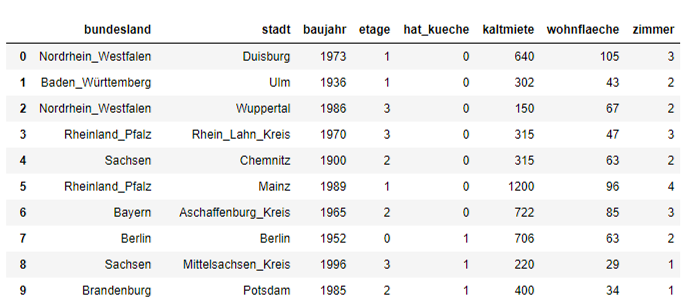
\includegraphics{bilder/dataframe.png}
\caption{Abbildung: Tabelle von Wohnungsangeboten}
\end{figure}

Hier wären die Aufgaben von Data Science:

\begin{itemize}
\tightlist
\item
  Daten ``verstehen'', Zusammenhänge zwischen
  Variablen aufdecken,
\item
  visualisieren.
\item
  Gegebenenfalls fehlende Einträge bei (z.B.) \texttt{kaltmiete} vorhersagen
\end{itemize}

\begin{figure}
\centering
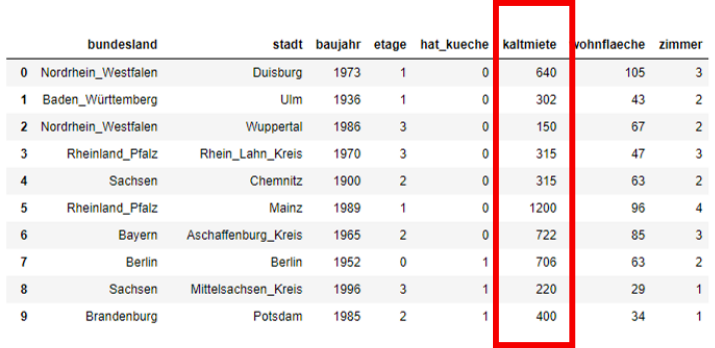
\includegraphics{bilder/dataframe_spalte.png}
\caption{Abbildung: Eine Spalte der Tabelle}
\end{figure}

Datenexploration und -analyse für einzelne Variablen 1/3 Wir betrachten
eine \emph{numerische} Variable in einem rechteckigen Datensatz, also eine
\emph{Spalte} (z.B. \texttt{kaltmiete}). Wir bezeichnen den \(i\)-ten Eintrag in
dieser Spalte mit \(x_i\), wobei \(i=1,\ldots,N\) (\(N\) Anzahl der Zeilen).

Folgende \emph{Schätzer}/\emph{Metriken} können dabei helfen, diese Spalte besser
zu verstehen:

\begin{itemize}
\item
  Mittelwert \(\overline x= \frac1 N\sum_{i=1}^N x_i\)
\item
  gewichteter Mittelwert
  \(\overline x_w = \frac{\sum_{i=1}^N w_i x_i}{\sum_{j=1}^N w_j}\),
  wobei \(w_i\) das Gewicht des \(i\)-ten Eintrages ist (z.B. eine andere
  Variable).
\item
  Varianz: \(s_x^2 = \frac{1}{N-1} \sum_{i=1}^N (x_i-\overline x)^2\)
\item
  Standardabweichung \(s = \sqrt{s_x^2}\).
\item
  Median = \(\frac{315 + 400}{2} = 357.5\).
\end{itemize}

Datenexploration und -analyse für mehrere Variablen Wir betrachten zwei
Spalten \(x = (x_1,\ldots,x_N)\) und \(y = (y_1,\ldots, y_N)\).\\

Das Verteilung von zwei Variablen läßt sich im sogenannte \textbf{Scatter Plot} visualisieren.

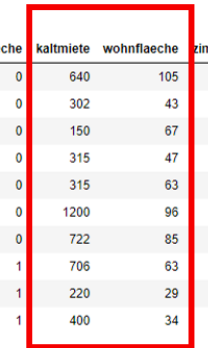
\includegraphics[width=0.27\textwidth,height=\textheight]{bilder/dataframe_spalte3.png}
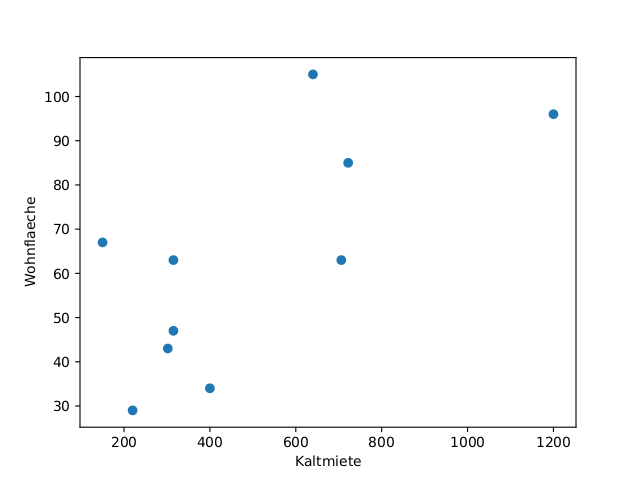
\includegraphics[width=0.7\textwidth,height=\textheight]{bilder/scatterplot.png}

Datenexploration und -analyse für mehrere Variablen Wir betrachten zwei
Spalten \(x = (x_1,\ldots,x_N)\) und \(y = (y_1,\ldots, y_N)\).

\begin{itemize}
\item
  Kovarianz
  \(s_{xy} = \frac{1}{N-1}\sum_{i=1}^N (x_i - \overline x)(y_i - \overline y)\)
\item
  Korrelation \(\rho_{xy} = \frac{s_{xy}}{s_x\cdot s_y} \in [-1,1]\).
\item
  \(\rho \approx 1\): Starke positive Korrelation, wenn \(x\) groß ist,
  ist \(y\) auch groß.
\item
  \(\rho \approx -1\): Starke negative Korrelation, wenn \(x\) groß ist,
  ist \(y\) klein
\item
  \(\rho \approx 0\): Wenig/keine Korrelation.
\end{itemize}

\begin{figure}
\centering
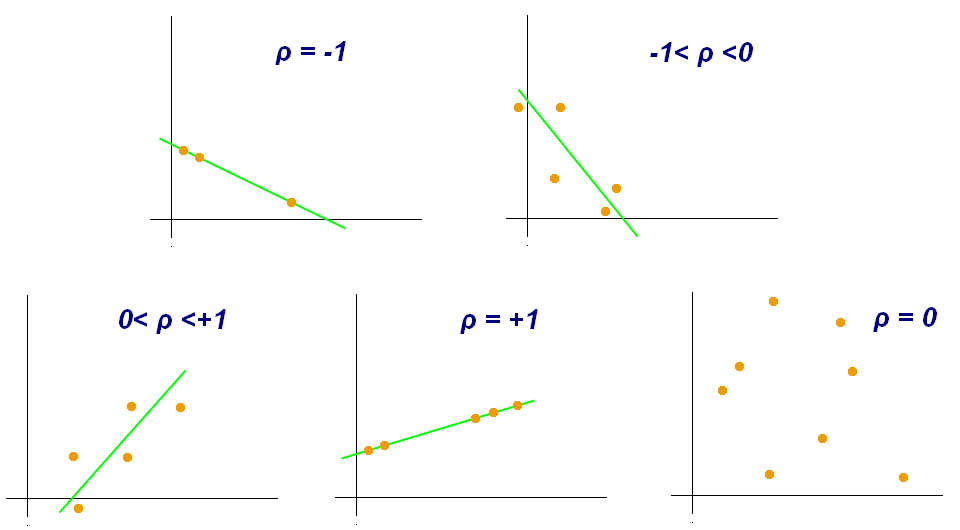
\includegraphics[width=0.65\textwidth,height=\textheight]{bilder/Correlation_coefficient.png}
\caption{Von Kiatdd - Eigenes Werk, CC BY-SA 3.0, \url{https://commons.wikimedia.org/w/index.php?curid=37108966}}
\end{figure}

\hypertarget{covid-19-daten}{%
\subsection{COVID-19 Daten}\label{covid-19-daten}}

Vergleiche die Einführung in \emph{Mathematik für Data Science 1} vom letzten Semester.

\hypertarget{netflix-prize}{%
\subsection{Netflix Prize}\label{netflix-prize}}

Hierbei geht es darum, ob aus bekannten Bewertungen von vielen verschiedenen Benutzern für viele verschiedene Filme abgeleitet werden kann, ob ein bestimmter Nutzer einen bestimmten Film mag (also positiv bewerten würde).

Vergleiche auch \href{https://en.wikipedia.org/wiki/Netflix_Prize}{Wikipedia:Netflix\_Prize}

Das (Trainings-)Daten bestehen über \texttt{480189} Benutzer, die für \texttt{17770} Filme insgesamt \texttt{100480507} Bewertungen als ganze Zahlen zwischen \texttt{1} und \texttt{5} verteilten.

Ziel der Datenanalyse war es, für \texttt{2817131} ``Paare'' von Benutzern und Filmen, die Bewertung vorauszusagen. Neben der schieren Masse an Daten kamen noch Einschränkungen hinzu, die ein Mindestmaß an Qualität der Vorhersage sicherstellen sollten.

Das Problem ließe sich wie folgt darstellen.

\begin{longtable}[]{@{}cccccc@{}}
\toprule
Benutzer \textbackslash{} Film & \texttt{F1} & \texttt{F2} & \texttt{...} & \texttt{Fn} & \texttt{...}\tabularnewline
\midrule
\endhead
\texttt{B1} & -- & 3 & \texttt{...} & 5 & \texttt{...}\tabularnewline
\texttt{B2} & 3 & 4 & \texttt{...} & 2 & \texttt{...}\tabularnewline
\texttt{B3} & 1 & 2 & \texttt{...} & \textbf{?} & \texttt{...}\tabularnewline
\texttt{...} & 3 & 4 & \texttt{...} & -- & \texttt{...}\tabularnewline
\bottomrule
\end{longtable}

Gegeben viele (aber bei weitem nicht alle) Einträge in einer riesigen Tabelle. Können wir aus den Zusammenhängen bestimmte fehlende Einträge (z.B. wie findet Nutzer \texttt{B3} den Film \texttt{Fn}) herleiten?

Die besten Lösungen für dieses Problem basieren durchweg auf \emph{Machine Learning} Ansätzen.

\hypertarget{python}{%
\section{Python}\label{python}}

Die Programmiersprache \texttt{python} wird uns durchs Semester begleiten. Einfach weil sie so wichtig ist für \emph{Data Science} aber auch weil sie (meiner Meinung nach) einfach zu erlernen und zu benutzen ist.

\hypertarget{aufgaben}{%
\section{Aufgaben}\label{aufgaben}}

\hypertarget{python-1}{%
\subsection{Python}\label{python-1}}

Bringen sie ihr \texttt{python} zum Laufen, installieren sie \texttt{numpy}, \texttt{scipy} und \texttt{matplotlib} und führen sie das folgende script aus.

\begin{Shaded}
\begin{Highlighting}[]
\ImportTok{import}\NormalTok{ numpy }\ImportTok{as}\NormalTok{ np}
\ImportTok{import}\NormalTok{ matplotlib.pyplot }\ImportTok{as}\NormalTok{ plt}

\NormalTok{N }\OperatorTok{=} \DecValTok{20}
\NormalTok{xmax }\OperatorTok{=} \DecValTok{2}
\NormalTok{xmin }\OperatorTok{=} \DecValTok{0}

\NormalTok{xdata }\OperatorTok{=}\NormalTok{ np.linspace(xmin, xmax, N)}
\NormalTok{ydata }\OperatorTok{=}\NormalTok{ np.exp(xdata)}

\NormalTok{plt.figure(}\DecValTok{1}\NormalTok{)}
\NormalTok{plt.plot(xdata, ydata, }\StringTok{\textquotesingle{}.\textquotesingle{}}\NormalTok{)}

\NormalTok{plt.figure(}\DecValTok{2}\NormalTok{)}
\NormalTok{plt.semilogy(xdata, ydata, }\StringTok{\textquotesingle{}.\textquotesingle{}}\NormalTok{)}
\NormalTok{plt.show()}
\end{Highlighting}
\end{Shaded}

\hypertarget{einheitsmatrix}{%
\subsection{Einheitsmatrix}\label{einheitsmatrix}}

Schreiben sie ein script, dass die \texttt{5x5} Einheitsmatrix auf 3 verschiedene Arten erzeugt. (Eine Art könnte die eingebaute \texttt{numpy} Funktion \texttt{eye} sein).

\begin{Shaded}
\begin{Highlighting}[]
\ImportTok{import}\NormalTok{ numpy }\ImportTok{as}\NormalTok{ np}

\NormalTok{idfive }\OperatorTok{=}\NormalTok{ np.eye(}\DecValTok{5}\NormalTok{)}
\BuiltInTok{print}\NormalTok{(idfive)}
\end{Highlighting}
\end{Shaded}

Hinweis: schauen sie sich mal an wie \texttt{numpy}'s \texttt{arrays} funktionieren.

\hypertarget{matrizen-multiplikation-und-potenz}{%
\subsection{Matrizen Multiplikation und Potenz}\label{matrizen-multiplikation-und-potenz}}

Schreiben sie ein script, das die Übungsaufgabe aus der Vorlesung (potenzieren der Matrizen \(M_i\), \(i=1,2,3,4\)) löst. Zum Beispiel mit

\begin{Shaded}
\begin{Highlighting}[]
\ImportTok{import}\NormalTok{ numpy }\ImportTok{as}\NormalTok{ np}
\NormalTok{mone }\OperatorTok{=}\NormalTok{ np.array([[}\FloatTok{0.9}\NormalTok{, }\FloatTok{0.9}\NormalTok{], [}\FloatTok{0.9}\NormalTok{, }\FloatTok{0.9}\NormalTok{]])}

\NormalTok{mone\_ptwo }\OperatorTok{=}\NormalTok{ mone }\OperatorTok{@}\NormalTok{ mone}
\BuiltInTok{print}\NormalTok{(mone\_ptwo)}

\NormalTok{mone\_pfour }\OperatorTok{=}\NormalTok{ mone\_ptwo }\OperatorTok{@}\NormalTok{ mone\_ptwo}
\BuiltInTok{print}\NormalTok{(mone\_pfour)}
\end{Highlighting}
\end{Shaded}

Oder so:

\begin{Shaded}
\begin{Highlighting}[]
\ImportTok{import}\NormalTok{ numpy }\ImportTok{as}\NormalTok{ np}
\NormalTok{mone }\OperatorTok{=}\NormalTok{ np.array([[}\FloatTok{0.9}\NormalTok{, }\FloatTok{0.9}\NormalTok{], [}\FloatTok{0.9}\NormalTok{, }\FloatTok{0.9}\NormalTok{]])}
\NormalTok{mone\_p }\OperatorTok{=}\NormalTok{ np.eye(}\DecValTok{2}\NormalTok{)}

\ControlFlowTok{for}\NormalTok{ k }\KeywordTok{in} \BuiltInTok{range}\NormalTok{(}\DecValTok{16}\NormalTok{):}
\NormalTok{    mone\_p }\OperatorTok{=}\NormalTok{ mone\_p }\OperatorTok{@}\NormalTok{ mone}
    \ControlFlowTok{if}\NormalTok{ k }\OperatorTok{==} \DecValTok{1} \KeywordTok{or}\NormalTok{ k }\OperatorTok{==} \DecValTok{3} \KeywordTok{or}\NormalTok{ k }\OperatorTok{==} \DecValTok{15}\NormalTok{:}
        \BuiltInTok{print}\NormalTok{(}\StringTok{\textquotesingle{}k=\textquotesingle{}}\NormalTok{, k}\OperatorTok{+}\DecValTok{1}\NormalTok{)}
        \BuiltInTok{print}\NormalTok{(mone\_p)}
\end{Highlighting}
\end{Shaded}

Achtung:

\begin{itemize}
\tightlist
\item
  bei Matrizen kann auch \texttt{*} benutzt werden -- das ist aber nicht die richtige Matrizenmultiplikation (sondern die Multiplikation eintragsweise)
\item
  Moegliche Realisierung der Matrizenmultiplikation

  \begin{itemize}
  \tightlist
  \item
    \texttt{np.dot(A,\ B)} -- die klassische Methode
  \item
    \texttt{A.dot(B)} -- das selbe (manchmal besser, wenn \texttt{A} etwas allgemeiner ist (zum Beispiel eine \texttt{scipy.sparse} matrix)
  \item
    \texttt{A\ @\ B} -- convenience Notation
  \end{itemize}
\end{itemize}

\hypertarget{sec-lineare-regression}{%
\chapter{Lineare Regression}\label{sec-lineare-regression}}

Auch bekannt als

\begin{itemize}
\tightlist
\item
  \emph{lineare Ausgleichsrechnung} oder
\item
  \emph{Methode der kleinsten Quadrate}.
\end{itemize}

Ein wesentlicher Aspekt von \emph{Data Science} ist die Analyse oder das
Verstehen von Daten. Allgemein gesagt, es wird versucht, aus den Daten
heraus Aussagen über Trends oder Eigenschaften des Phänomens zu treffen,
mit welchem die Daten im Zusammenhang stehen.

Wir kommen nochmal auf das Beispiel aus der Einführungswoche zurück, werfen eine bereits geschärften Blick darauf und gehen das mit verbesserten mathematischen Methoden an.

Gegeben seien die Fallzahlen aus der CoVID Pandemie 2020 für Bayern für den Oktober 2020.

\hypertarget{tab:covid-cases}{}
\begin{longtable}[]{@{}llllllllllll@{}}
\caption{Anzahl der SARS-CoV-2 Neuinfektionen in Bayern im Oktober 2020.}\tabularnewline
\toprule
Tag & 1 & 2 & 3 & 4 & 5 & 6 & 7 & 8 & 9 & 10 & 11\tabularnewline
\midrule
\endfirsthead
\toprule
Tag & 1 & 2 & 3 & 4 & 5 & 6 & 7 & 8 & 9 & 10 & 11\tabularnewline
\midrule
\endhead
Fälle & 352 & 347 & 308 & 151 & 360 & 498 & 664 & 686 & 740 & 418 & 320\tabularnewline
\bottomrule
\end{longtable}

\begin{longtable}[]{@{}lllllllllll@{}}
\toprule
Tag & 12 & 13 & 14 & 15 & 16 & 17 & 18 & 19 & 20 & 21\tabularnewline
\midrule
\endhead
Fälle & 681 & 691 & 1154 & 1284 & 127 & 984 & 573 & 1078 & 1462 & 2239\tabularnewline
\bottomrule
\end{longtable}

\begin{longtable}[]{@{}lllllllllll@{}}
\toprule
Tag & 22 & 23 & 24 & 25 & 26 & 27 & 28 & 29 & 30 & 31\tabularnewline
\midrule
\endhead
Fälle & 2236 & 2119 & 1663 & 1413 & 2283 & 2717 & 3113 & 2972 & 3136 & 2615\tabularnewline
\bottomrule
\end{longtable}

\begin{figure}
\hypertarget{fig:cases}{%
\centering
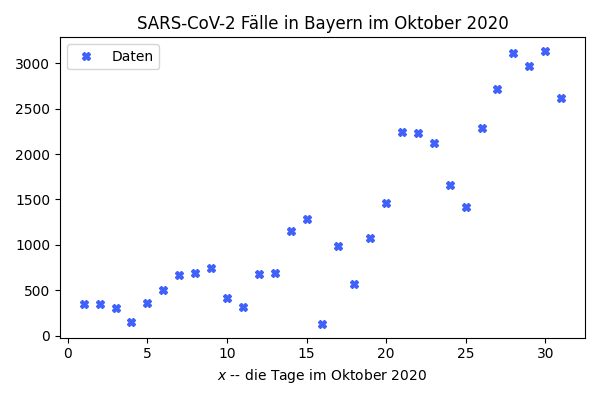
\includegraphics{bilder/02-cases.png}
\caption{Fallzahlen von Sars-CoV-2 in Bayern im Oktober
2020}\label{fig:cases}
}
\end{figure}

Wieder stellen wir uns die Frage ob wir \textbf{in den Daten einen funktionalen
Zusammenhang} feststellen können. Also ob wir die Datenpaare

\begin{quote}
(Tag \(x\), Infektionen am Tag \(x\))
\end{quote}

die wir als

\begin{quote}
(\(x_i\), \(y_i\))
\end{quote}

über eine Funktion \(f\) und die Paare

\begin{quote}
(\(x\), \(f(x)\))
\end{quote}

beschreiben (im Sinne von gut darstellen oder approximieren) können.

\hypertarget{rauschen-und-fitting}{%
\section{Rauschen und Fitting}\label{rauschen-und-fitting}}

Beim obigen Beispiel (und ganz generell bei Daten) ist davon auszugehen, dass die Daten \textbf{verrauscht} sind, also einem Trend folgen oder in einem funktionalen Zusammenhang stehen aber zufällige Abweichungen oder Fehler enthalten.

Unter diesem Gesichtspunkt ist eine Funktion, die

\begin{quote}
\(f(x_i)=y_i\)
\end{quote}

erzwingt nicht zielführend. (Wir wollen Trends und größere Zusammenhänge erkennen und nicht kleine Fehler nachzeichnen.) Das zu strenge Anpassen an möglicherweise verrauschte Daten wird \textbf{overfitting} genannt.

Vielmehr werden wir nach einer Funktion \(f\) suchen, die die Daten näherungsweise nachstellt:

\begin{quote}
\(f(x_i)\approx y_i\)
\end{quote}

Hierbei passen jetzt allerdings auch Funktionen, die vielleicht einfach zu handhaben sind aber die Daten kaum noch repräsentieren. Jan spricht von \textbf{underfitting}.

Eine gute Approximation besteht im Kompromiss von \emph{nah an den Daten} aber mit wenig \emph{overfitting}.

\hypertarget{ansuxe4tze-fuxfcr-lineare-regression}{%
\section{Ansätze für lineare Regression}\label{ansuxe4tze-fuxfcr-lineare-regression}}

Um eine solche Funktion \(f\) zu finden, trifft Jan als erstes ein paar
Modellannahmen. Modellannahmen legen fest, wie das \(f\) im Allgemeinen
aussehen soll und versuchen dabei

\begin{enumerate}
\def\labelenumi{\arabic{enumi}.}
\item
  die Bestimmung von \(f\) zu ermöglichen
\item
  zu garantieren, dass \(f\) auch die gewollten Aussagen liefert
\item
  und sicherzustellen, dass \(f\) zum Problem passt.
\end{enumerate}

Jan bemerke, dass die ersten beiden Annahmen im Spannungsverhältnis zur
dritten stehen.

\textbf{Lineare Regression} besteht darin, dass die Funktion als Linearkombination

\begin{equation*}
f_w(x) = \sum_{j=1}^n w_j b_j(x)
\end{equation*}

von Basisfunktionen geschrieben wird und dann die \emph{Koeffizienten} \(w_i\) so bestimmt werden, dass \(f\) die Daten bestmöglich annähert.

\begin{quote}
Jan bemerke, dass \emph{bestmöglich} wieder \emph{overfitting} bedeuten kann aber auch, bei schlechter Wahl der Basis, wenig aussagekräftig sein kann. Der gute Kompromiss liegt also jetzt in der Wahl der passenden Basisfunktionen und deren Anzahl. (Mehr Basisfunktionen bedeutet möglicherweise bessere Approximation aber auch die Gefahr von \emph{overfitting}.)
\end{quote}

Typische Wahlen für die Basis \(\{b_1, b_2, \dotsc, b_n\}\) sind

\begin{itemize}
\tightlist
\item
  Polynome: \(\{1, x, x^2, \dotsc, x^{n-1}\}\) -- für \(n=2\) ist der Ansatz \emph{eine Gerade}
\item
  Trigonometrische Funktionen: \(\{1, \cos(x), \sin(x), \cos(2x), \sin(2x), \dotsc\}\)
\item
  Splines -- Polynome, die abschnittsweise definiert werden
\item
  Wavelets -- Verallgemeinerungen von trigonometrischen Funktionen
\end{itemize}

\hypertarget{sec-linreg-minimierung}{%
\section{Fehlerfunktional und Minimierung}\label{sec-linreg-minimierung}}

Wir setzen nun also an
\begin{equation*}
f_w(x) = \sum_{j=1}^nw_j b_j (x)
\end{equation*}
und wollen damit \(y_i \approx f_w(x_i)\) \emph{bestmöglich} erreichen (indem wir die Koeffizienten \((w_1, \dotsc, w_n)\) \emph{optimal} wählen. Bestmöglich und optimal spezifizieren wir über den Mittelwert der quadratischen Abweichungen in der Approximation über alle Datenpunkte
\begin{equation*}
\frac{1}{N}\sum_{i=1}^N (y_i - f_w(x_i))^2
\end{equation*}

Ein paar Bemerkungen

\begin{itemize}
\tightlist
\item
  jetzt müssen wir die \(w_i\)'s bestimmen so dass dieser Fehlerterm minimal wird
\item
  das optimale \(w\) ist unabhängig von einer Skalierung des Fehlerterms
\item
  des wegen schreiben wir gerne einfach \(\frac 12 \sum_{i=1}^N (y_i - f_w(x_i))^2\) als das Zielfunktional, das es zu minimieren gilt.
\end{itemize}

Wie finden wir jetzt die \(w_i\)'s? Zunächst gilt, dass
\begin{equation*}
f_w(x_i) = \sum_{i=j}^n w_j b_j(x_i) = 
\begin{bmatrix}
b_1(x_i) & b_2(x_i) & \dots & b_n(x_i)
\end{bmatrix}
\begin{bmatrix}
w_1 \\ w_2 \\ \vdots \\ w_n
\end{bmatrix}
\end{equation*}

und wenn wir alle \(f_w(x_i)\), \(i=1,\dotsc,N\) übereinander in einen Vektor schreiben, dass

\begin{equation*}
f_w(\mathbf x) := 
\begin{bmatrix}
f_w(x_1) \\ \vdots \\ f_w(x_N)
\end{bmatrix}
=
\begin{bmatrix}
b_1(x_1) & \dots & b_n(x_1) \\
\vdots & \ddots & \vdots \\
b_1(x_N) & \dots & b_n(x_N)
\end{bmatrix}
\begin{bmatrix}
w_1 \\ \vdots \\ w_n
\end{bmatrix}
=: \Phi(\mathbf x) w
\end{equation*}

Damit, mit \(\mathbf y\) als den Vektor aller \(y_i\)'s, und mit der Definition der Vektornorm, können wir unser Minimierungsproblem schreiben als
\begin{equation*}
\frac 12  \sum_{i=1}^N (y_i - f_w(x_i))^2 = \frac 12 \| \mathbf y - \Phi (\mathbf x) w\|^2 \to \min.
\end{equation*}

Wir bemerken, dass

\begin{itemize}
\tightlist
\item
  das Fehlerfunktional immer größer und bestenfalls gleich 0 ist
\item
  falls das lineare Gleichungssystem \(\Phi (\mathbf x)w = \mathbf y\) eine Lösung \(w\) hat, ist das auch eine Lösung unserer Minimierung
\item
  im typischen Falle aber ist allerdings \(N\gg n\) und das System überbestimmt (\(n=N\) würde ein overfitting bedeuten\ldots) sodass wir keine Lösung des linearen Gleichungssystems erwarten können.
\item
  Das Minimierungsproblems selbst hat allerdings immer eine Lösung.
\end{itemize}

\hypertarget{berechnung-der-bestluxf6sung}{%
\section{Berechnung der Bestlösung}\label{berechnung-der-bestluxf6sung}}

Wir suchen also ein Minimum der Funktion (mit \(\Phi\), \(\mathbf x\), \(\mathbf y\) gegeben)
\begin{equation*}
\begin{split}
w \mapsto \frac 12 \|\mathbf y - \Phi(\mathbf x)w \|^2 &= \frac 12 (\mathbf y - \Phi(\mathbf x)w)^T(\mathbf y - \Phi(\mathbf x)w)  \\ 
&= \frac 12 [\mathbf y^T\mathbf y - \mathbf y^T \Phi(\mathbf x)w - w^T \Phi(\mathbf x)^T\mathbf y  + w^T \Phi(\mathbf x)^T\Phi(\mathbf x)w] \\
&= \frac 12 [\mathbf y^T\mathbf y -2 w^T \Phi(\mathbf x)^T\mathbf y  + w^T \Phi(\mathbf x)^T\Phi(\mathbf x)w] 
\end{split}
\end{equation*}
wobei wir die Definition der Norm \(\|v\|^2 = v^Tv\) und die Eigenschaft, dass für die skalare Größe \(w^T \Phi(\mathbf x)^T\mathbf y = [w^T \Phi(\mathbf x)^T\mathbf y]^T = \mathbf y^T \Phi(\mathbf x)w\) gilt, ausgenutzt haben.

Wären \(w\) und \(\mathbf y\) keine Vektoren sondern einfach reelle Zahlen, wäre das hier eine Parabelgleichung \(aw^2 + bw + c\) mit \(a>0\), die immer eine Minimalstelle hat.

Tatsächlich gilt hier alles ganz analog. Insbesondere ist \(\Phi(\mathbf x)^T\Phi(\mathbf x)\) in der Regel ``größer 0'' (was heißt das wohl bei quadratischen Matrizen?). Und mittels ``Nullsetzen'' der ersten Ableitung können wir das Minimum bestimmen. In diesem Fall ist die erste Ableitung (nach \(w\))
\begin{equation*}
\nabla_w (\frac 12 \|\mathbf y - \Phi(\mathbf x) \|^2) = \Phi(\mathbf x)^T\Phi(\mathbf x)w - \Phi(\mathbf x)^T\mathbf y,
\end{equation*}
(den \emph{Gradienten} \(\nabla_w\) als Ableitung von Funktionen mit mehreren Veränderlichen werden wir noch genauer behandeln)
was uns als Lösung, die Lösung des linearen Gleichungssystems
\begin{equation*}
\Phi(\mathbf x)^T\Phi(\mathbf x)w = \Phi(\mathbf x)^T\mathbf y
\end{equation*}
definiert.

Letzte Frage: Wann hat dieses Gleichungssystems eine eindeutige Lösung? Mit \(N>n\) (also \(\Phi(\mathbf x)\) hat mehr Zeilen als Spalten) gelten die Äquivalenzen:

\begin{itemize}
\tightlist
\item
  \(\Phi(\mathbf x)^T\Phi(\mathbf x)w = \Phi(\mathbf x)^T\mathbf y\) hat eine eindeutige Lösung
\item
  die Matrix \(\Phi(\mathbf x)^T\Phi(\mathbf x)\) ist regulär
\item
  die Spalten von \(\Phi(\mathbf x)\) sind linear unabhängig
\item
  die Vektoren \(b_i(\mathbf x)\) sind linear unabhängig.
\end{itemize}

Praktischerweise tritt genau diese Situation im Allgemeinen ein.

\begin{itemize}
\tightlist
\item
  \(N>n\) (mehr Datenpunkte als Parameter)
\item
  \(b_i\)'s werden als \emph{linear unabhängig} (im Sinne ihres Funktionenraums) gewählt, was die lineare unabhängigket der \(b_i(\mathbf x)\) impliziert.
\end{itemize}

\hypertarget{beispiel}{%
\section{Beispiel}\label{beispiel}}

Unsere Covid-Zahlen ``mit einer Geraden angenähert'':

\begin{itemize}
\tightlist
\item
  \(f_w(x) = w_1 + w_2 x\) -- das heißt \(n=2\) und Basisfunktionen \(b_1(x)\equiv 1\) und \(b_2(x) = x\)
\item
  \(\mathbf x = (1,2,3, \dots, 31)\) -- die Tage im Februar, das heißt \(N=31\)
\item
  \(\mathbf y = (352, 347, \dots, 2615)\) -- die Fallzahlen
\end{itemize}

Wir bekommen

\begin{equation*}
\Phi(\mathbf x) = 
\begin{bmatrix}
1 & 1 \\ 1 & 2 \\ 1 & 3 \\ \vdots & \vdots \\ 1 & 31
\end{bmatrix}
\end{equation*}
(die Spalten sind linear unabhängig) und müssen ``nur'' das 2x2 System
\[
\begin{bmatrix}
1 & 1 & 1 & \dots & 1 \\ 1 & 2 & 3 & \dots & 31
\end{bmatrix}
\begin{bmatrix}
1 & 1 \\ 1 & 2 \\ 1 & 3 \\ \vdots \\ 1 & 31
\end{bmatrix}
\begin{bmatrix}
w_1 \\ w_2
\end{bmatrix}
=
\begin{bmatrix}
1 & 1 & 1 & \dots & 1 \\ 1 & 2 & 3 & \dots & 31
\end{bmatrix} 
\begin{bmatrix}
352 \\  347 \\ 308 \\ \vdots \\ 2615
\end{bmatrix} 
\]
lösen um die Approximation \(f_w\) zu bestimmen.

Und noch als letzte Bemerkung. Egal wie die Basisfunktionen \(b_i\) gewählt werden, die Parameterabhängigkeit von \(w\) ist immer linear. Deswegen der Name \textbf{lineare Ausgleichsrechnung}.

\hypertarget{matrix-zerlegungen}{%
\chapter{Matrix-Zerlegungen}\label{matrix-zerlegungen}}

Die Lösung \(w\) des Problems der \emph{linearen Ausgleichsrechnung} war entweder als Lösung eines Optimierungsproblems
\begin{equation*}
\min_{w} \| Aw - y \|^2
\end{equation*}
oder als Lösung des linearen Gleichungssystems
\begin{equation*}
A^TAw=y
\end{equation*}
gegeben. Hierbei steht nun \(A\in \mathbb R^{N\times n}\) für die Matrix \(\Phi(\mathbf x)\) der Daten und Basisfunktionen. Wir hatten uns überlegt, dass in den meisten Fällen

\begin{itemize}
\tightlist
\item
  die Matrix mehr Zeilen als Spalten hat (\(N>n\)) und
\item
  die Spalten linear unabhängig sind.
\end{itemize}

\hypertarget{qr-zerlegung}{%
\section{QR Zerlegung}\label{qr-zerlegung}}

Wir betrachten nochmal das Optimierungsproblem \(\min_{w} \| Aw - y \|^2\). Gäbe es eine Lösung des Systems \(Aw=y\), wäre das sofort eine Lösung des Optimierungsproblems. Da \(A\) aber mehr Zeilen als Spalten hat, ist das System \(Aw=y\) überbestimmt und eine Lösung in der Regel nicht gegeben.

Die Überlegung ist nun, die Gleichung \(Aw=y\) \emph{so gut wie möglich} zu erfüllen, indem wir die relevanten Gleichungen indentifizieren und wenigstens diese lösen. Ein systematischer (und wie wir später sehen werden auch zum Optimierungsproblem passender) Zugang bietet die QR Zerlegung.

\begin{theorem}[QR Zerlegung]
\protect\hypertarget{thm:qr}{}\label{thm:qr}Sei \(A\in \mathbb R^{m\times n}\), \(m>n\). Dann existiert eine orthonormale Matrix \(Q\in \mathbb R^{m\times m}\) und eine obere Dreiecksmatrix \(\hat R\in \mathbb R^{n\times n}\) derart dass
\begin{equation*}
A = QR =: Q 
\begin{bmatrix}
\hat R \\ 0
\end{bmatrix}.
\end{equation*}
Hat \(A\) vollen (Spalten)Rang, dann ist \(\hat R\) invertierbar.
\end{theorem}

Hier heißt \emph{orthonormale Matrix} \(Q\), dass die Spalten von \(Q\) paarweise orthogonal sind. Insbesondere gilt
\begin{equation*}
Q^T Q = I.
\end{equation*}

Für unser zu lösendes Problem ergibt sich dadurch die Umformung
\begin{equation*}
Aw = y \quad \Leftrightarrow \quad QRw=y \quad \Leftrightarrow \quad Q^TQRw=Q^T y 
 \quad \Leftrightarrow \quad  Rw = Q^Ty
\end{equation*}
oder auch
\begin{equation*}
\begin{bmatrix}
\hat R \\ 0
\end{bmatrix}w 
=
Q^Ty
=
\begin{bmatrix}
Q_1^T \\ Q_2^T
\end{bmatrix}
y
\end{equation*}
(wobei wir die \(Q_1\in \mathbb R^{m\times n}\) die Matrix der ersten \(n\) Spalten von \(Q\) ist)
und als \emph{Kompromiss} der Vorschlag, das Teilsystem
\begin{equation*}
\hat R w = Q_1^Ty
\end{equation*}
nach \(w\) zu lösen und in Kauf zu nehmen, dass der Rest, nämlich das \(Q_2^Ty\), nicht notwendigerweise gleich null ist.

Wir halten zunächst mal fest, dass

\begin{itemize}
\tightlist
\item
  Obwohl \(Q\) eine reguläre Matrix ist, bedarf der Übergang von \(Aw=y\) zu \(Q^TAw=Q^Ty\) einer genaueren Analyse.
\item
  Wir bemerken, dass für eine hypothetische komplette Lösung \(Aw-y\), diese Transformation keine Rolle spielt.
\item
  Für die Kompromisslösung jedoch schon, weil beispielsweise verschiedene Konstruktionen eines invertierbaren Teils, verschiedene Residuen bedeuten und somit Optimalität im Sinne von \(\min_w \|Aw-y\|^2\) nicht garantiert ist.
\end{itemize}

Allerdings, wie Sie als Übungsaufgabe nachweisen werden, löst dieser Ansatz tatsächlich das Optimierungsproblem.

\hypertarget{singuluxe4rwertzerlegung}{%
\section{Singulärwertzerlegung}\label{singuluxe4rwertzerlegung}}

Eine weitere Matrix Zerlegung, die eng mit der Lösung von Optimierungsproblemen oder überbestimmten Gleichungssystemen zusammenhängt ist die \emph{Singulärwertzerlegung} (SVD -- von english: \emph{Singular Value Decomposition}).

\begin{theorem}[Singulärwertzerlegung]
\protect\hypertarget{thm:SVD}{}\label{thm:SVD}Sei \(A\in \mathbb C^{m\times n}\), \(m\geq n\). Dann existieren orthogonale Matrizen \(U \in \mathbb C^{m\times m}\) und \(V\in \mathbb C^{n\times n}\) und eine Matrix \(\Sigma \in \mathbb R^{m\times n}\) der Form
\begin{equation*}
\Sigma = 
\begin{bmatrix}
\sigma_1 & 0 & \dots & 0\\
0 & \sigma_2 &\ddots & \vdots\\
0 & \ddots & \ddots &0\\
  0 & \dots&0 & \sigma_n \\
  0 & 0 & \dots & 0 \\
  \vdots & \ddots &  & \vdots\\
  0 & 0 & \dots & 0
\end{bmatrix}
\end{equation*}
mit reellen sogenannten \emph{Singulärwerten}
\begin{equation*}
\sigma_1 \geq \sigma_2 \geq \dots \geq \sigma_n \geq 0
\end{equation*}
sodass gilt
\begin{equation*}
A = U \Sigma V^*
\end{equation*}
wobei gilt \(V^* = \overline{V^T}\) (transponiert und komplex konjugiert).
\end{theorem}

Ein paar Bemerkungen.

\begin{itemize}
\tightlist
\item
  Ist \(A\) reell, können auch \(U\) und \(V\) reell gewählt werden.
\item
  Die Annahme \(m \geq n\) war nur nötig um für die Matrix \(\Sigma\) keine Fallunterscheidung zu machen. (Für \(m\leq n\) ``steht der Nullblock rechts von den Singulärwerten''). Insbesondere gilt \(A^* = V\Sigma U^*\) ist eine SVD von \(A^*\).
\item
  Eine Illustration der Zerlegung ist \href{@fig-SVD}{hier} zu sehen.
\end{itemize}

Wir machen einige Überlegungen im Hinblick auf große Matrizen. Sei dazu \(m>n\), \(A\in \mathbb C^{m\times n}\) und \(A=U\Sigma V^*\) eine SVD wie in Theorem \ref{thm:SVD}. Sei nun
\begin{equation*}
U = \begin{bmatrix}
U_1 & U_2
\end{bmatrix}
% = \begin{bmatrix} V_1^* & V_2^*
\end{equation*}
partitioniert sodass \(U_1\) die ersten \(n\) Spalten von \(U\) enthält.

Dann gilt (nach der Matrix-Multiplikations Regel \emph{Zeile mal Spalte} die Teile \(U_2\) und \(V_2\) immer mit dem Nullblock in \(\Sigma\) multipliziert werden) dass
\begin{equation*}
A = U\Sigma V = 
\begin{bmatrix}
U_1 & U_2
\end{bmatrix}
\begin{bmatrix}
\hat \Sigma \\ 0
\end{bmatrix}
V^*
% \begin{bmatrix} V_1^* \\ V_2^* \end{bmatrix}
=
U_1 
\hat \Sigma
V^*
% \begin{bmatrix} V_1^* \\ V_2^* \end{bmatrix}
\end{equation*}
Es genügt also nur die ersten \(m\) Spalten von \(U\) zu berechnen. Das ist die sogenannte \textbf{slim SVD}.

Hat, darüberhinaus, die Matrix \(A\) keinen vollen Rang, also \(\operatorname{Rg}(A) = r < n\), dann:

\begin{itemize}
\tightlist
\item
  ist \(\sigma_i=0\), für alle \(i=r+1, \dotsc, n\), (wir erinnern uns, dass die Singulärwerte nach Größe sortiert sind)
\item
  die Matrix \(\hat \Sigma\) hat \(n-r\) Nullzeilen
\item
  für die Zerlegung sind nur die ersten \(r\) Spalten von \(U\) und \(V\) relevant -- die sogenannte \textbf{Kompakte SVD}.
\end{itemize}

In der Datenapproximation ist außerdem die \textbf{truncated SVD} von Interesse. Dazu sei \(\hat r<r\) ein beliebig gewählter Index. Dann werden alle Singulärwerte, \(\sigma_i=0\), für alle \(i=\hat r+1, \dotsc, n\), abgeschnitten -- das heißt null gesetzt und die entsprechende \emph{kompakte SVD} berechnet.

Hier gilt nun nicht mehr die Gleichheit in der Zerlegung. Vielmehr gilt
\begin{equation*}
A \approx A_{\hat r}
\end{equation*}
wobei \(A_{\hat r}\) aus der \emph{truncated SVD} von \(A\) erzeugt wurde. Allerdings ist diese Approximation von \(A\) durch optimal in dem Sinne, dass es keine Matrix vom Rang \(\hat r \geq r=\operatorname{Rg}(A)\) gibt, die \(A\) (in der \emph{induzierten} euklidischen Norm\footnote{Auf Matrixnormen kommen wir noch in der Vorlesung zu sprechen.}) besser approximiert. Es gilt
\begin{equation*}
\min_{B\in \mathbb C^{m\times n}, \operatorname{Rg}(B)=\hat r} \|A-B\|_2 = \|A-A_{\hat r}\|_2 = \sigma_{\hat r + 1};
\end{equation*}
(vgl. Satz 14.15, Bollhöfer and Mehrmann \protect\hyperlink{ref-BolM04}{2004}).

Zum Abschluss noch der Zusammenhang zum Optimierungsproblem. Ist \(A=U\Sigma V^*\) ``SV-zerlegt'', dann gilt
\begin{equation*}
A^*Aw = V\Sigma^*U^*U\Sigma V^*w = V\hat \Sigma^2 V^* 
\end{equation*}
und damit
\begin{equation*}
A^*Aw = A^*y \quad \Leftrightarrow \quad V\hat \Sigma^2 V^*  = V\Sigma^*U^*y \quad \Leftrightarrow \quad w = V(\Sigma^+)^*U^*y
\end{equation*}
wobei
\begin{equation*}
\Sigma^+ = \begin{bmatrix}
\hat \Sigma^{-1} \\ 0_{m-n \times n}
\end{bmatrix}
\end{equation*}
aus \(\Sigma \hat \Sigma^{-1}\hat \Sigma^{-1}\) herrührt.

\textbf{Bemerkung}: \(\Sigma^+\) kann auch definiert werden, wenn \(\hat \Sigma\) nicht invertierbar ist (weil manche Diagonaleinträge null sind). Dann wird \(\hat \Sigma^+\) betrachtet, bei welcher nur die \(\sigma_i>0\) invertiert werden und die anderen \(\sigma_i=0\) belassen werden. Das definiert eine sogenannte \emph{verallgemeinerte Inverse} und löst auch das Optimierungsproblem falls \(A\) keinen vollen Rang hat.

\begin{figure}
\hypertarget{fig-SVD}{%
\centering
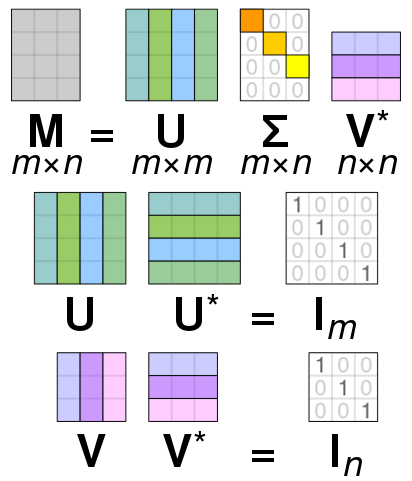
\includegraphics[width=0.5\textwidth,height=\textheight]{bilder/03-412px-Singular_value_decomposition_visualisation.svg.png}
\caption{Illustration der SVD. Bitte beachten der \(*\) bedeutet hier transponiert und komplex konjugiert. By Cmglee - Own work, CC BY-SA 4.0, \url{https://commons.wikimedia.org/w/index.php?curid=67853297}}\label{fig-SVD}
}
\end{figure}

\hypertarget{aufgaben-1}{%
\section{Aufgaben}\label{aufgaben-1}}

Erklärung: (T) heißt theoretische Aufgabe, (P) heißt programmieren.

\hypertarget{norm-und-orthogonale-transformation-t}{%
\subsection{Norm und Orthogonale Transformation (T)}\label{norm-und-orthogonale-transformation-t}}

Sei \(Q\in \mathbb R^{n\times n}\) eine orthogonale Matrix und sei \(y\in \mathbb R^{n}\). Zeigen Sie, dass
\begin{equation*}
\|y\|^2 = \|Qy \|^2
\end{equation*}
gilt. (2 Punkte)

\hypertarget{kleinste-quadrate-und-mittelwert}{%
\subsection{Kleinste Quadrate und Mittelwert}\label{kleinste-quadrate-und-mittelwert}}

Zeigen sie, dass der \emph{kleinste Quadrate} Ansatz zur Approximation einer Datenwolke
\begin{equation*}
(x_i, y_i), \quad i=1,2,\dotsc,N,
\end{equation*}
mittels einer konstanten Funktion \(f(x)=w_1\) auf \(w_1\) auf den Mittelwert der \(y_i\) führt. (6 Punkte)

\hypertarget{qr-zerlegung-und-kleinstes-quadrate-problem-t}{%
\subsection{QR Zerlegung und Kleinstes Quadrate Problem (T)}\label{qr-zerlegung-und-kleinstes-quadrate-problem-t}}

Sei \(A\in \mathbb R^{m,n}\), \(m>n\), \(A\) hat vollen Rank und sei
\begin{equation*}
\begin{bmatrix}
Q_1 & Q_2
\end{bmatrix}
\begin{bmatrix}
\hat R \\ 0
\end{bmatrix} = A
\end{equation*}
eine QR-Zerlegung von \(A\). Zeigen sie, dass die Lösung von
\begin{equation*}
\hat R w = Q_1^T y
\end{equation*}
ein kritischer Punkt (d.h. der Gradient \(\nabla_w\) verschwindet) von
\begin{equation*}
w \mapsto \frac 12 \| Aw - y \|^2
\end{equation*}
ist. \textbf{Hinweis}: Die Formel für den Gradienten wurde in der Vorlesung 02 hergeleitet. (6 Punkte)

\hypertarget{eigenwerte-symmetrischer-matrizen-t}{%
\subsection{Eigenwerte Symmetrischer Matrizen (T)}\label{eigenwerte-symmetrischer-matrizen-t}}

Zeigen Sie, dass Eigenwerte symmetrischer reeller Matrizen \(A\in \mathbb R^{n\times n}\) immer reell sind. (3 Punkte)

\hypertarget{singuluxe4rwertzerlegung-und-eigenwerte-t}{%
\subsection{Singulärwertzerlegung und Eigenwerte (T)}\label{singuluxe4rwertzerlegung-und-eigenwerte-t}}

Zeigen Sie, dass die quadrierten Singulärwerte einer Matrix \(A\in \mathbb R^{m\times n}\), \(m>n\), genau die Eigenwerte der Matrix \(A^TA\) sind und in welcher Beziehung sie mit den Eigenwerten von \(AA^T\) stehen. \textbf{Hinweis}: hier ist ``\(m>n\)'' wichtig. (6 Punkte)

\hypertarget{python-laden-und-speichern-von-arrays}{%
\subsection{Python -- Laden und Speichern von Arrays}\label{python-laden-und-speichern-von-arrays}}

Speichern sie die Covid-Daten aus obiger Tabelle zur späteren Verwendung als ein \texttt{numpy.array}. Beispielsweise so:

\begin{Shaded}
\begin{Highlighting}[]
\ImportTok{import}\NormalTok{ numpy }\ImportTok{as}\NormalTok{ np}
\ImportTok{import}\NormalTok{ matplotlib.pyplot }\ImportTok{as}\NormalTok{ plt}

\NormalTok{days }\OperatorTok{=}\NormalTok{ [}\DecValTok{1}\NormalTok{, }\DecValTok{2}\NormalTok{, }\DecValTok{3}\NormalTok{, }\DecValTok{4}\NormalTok{, }\DecValTok{5}\NormalTok{, }\DecValTok{6}\NormalTok{, }\DecValTok{7}\NormalTok{, }\DecValTok{8}\NormalTok{, }\DecValTok{9}\NormalTok{, }\DecValTok{10}\NormalTok{, }\DecValTok{11}\NormalTok{,}
        \DecValTok{12}\NormalTok{, }\DecValTok{13}\NormalTok{, }\DecValTok{14}\NormalTok{, }\DecValTok{15}\NormalTok{,  }\DecValTok{16}\NormalTok{, }\DecValTok{17}\NormalTok{, }\DecValTok{18}\NormalTok{, }\DecValTok{19}\NormalTok{,  }\DecValTok{20}\NormalTok{,   }\DecValTok{21}\NormalTok{,}
        \DecValTok{22}\NormalTok{,  }\DecValTok{23}\NormalTok{,  }\DecValTok{24}\NormalTok{,   }\DecValTok{25}\NormalTok{,    }\DecValTok{26}\NormalTok{, }\DecValTok{27}\NormalTok{,  }\DecValTok{28}\NormalTok{,   }\DecValTok{29}\NormalTok{,    }\DecValTok{30}\NormalTok{,     }\DecValTok{31}\NormalTok{]}
\NormalTok{case }\OperatorTok{=}\NormalTok{ [}\DecValTok{352}\NormalTok{, }\DecValTok{347}\NormalTok{, }\DecValTok{308}\NormalTok{, }\DecValTok{151}\NormalTok{, }\DecValTok{360}\NormalTok{, }\DecValTok{498}\NormalTok{, }\DecValTok{664}\NormalTok{, }\DecValTok{686}\NormalTok{, }\DecValTok{740}\NormalTok{, }\DecValTok{418}\NormalTok{, }\DecValTok{320}\NormalTok{,}
        \DecValTok{681}\NormalTok{, }\DecValTok{691}\NormalTok{, }\DecValTok{1154}\NormalTok{, }\DecValTok{1284}\NormalTok{,  }\DecValTok{127}\NormalTok{, }\DecValTok{984}\NormalTok{, }\DecValTok{573}\NormalTok{, }\DecValTok{1078}\NormalTok{,  }\DecValTok{1462}\NormalTok{,   }\DecValTok{2239}\NormalTok{,}
        \DecValTok{2236}\NormalTok{,  }\DecValTok{2119}\NormalTok{,  }\DecValTok{1663}\NormalTok{,   }\DecValTok{1413}\NormalTok{,    }\DecValTok{2283}\NormalTok{,}
        \DecValTok{2717}\NormalTok{,  }\DecValTok{3113}\NormalTok{,   }\DecValTok{2972}\NormalTok{,    }\DecValTok{3136}\NormalTok{,    }\DecValTok{2615}\NormalTok{]}

\NormalTok{data }\OperatorTok{=}\NormalTok{ np.vstack([days, case])}
\BuiltInTok{print}\NormalTok{(}\StringTok{\textquotesingle{}Shape of data: \textquotesingle{}}\NormalTok{, data.shape)}

\NormalTok{datafilestr }\OperatorTok{=} \StringTok{\textquotesingle{}coviddata.npy\textquotesingle{}}
\NormalTok{np.save(datafilestr, data)}

\NormalTok{lddata }\OperatorTok{=}\NormalTok{ np.load(datafilestr)}

\NormalTok{plt.figure(}\DecValTok{1}\NormalTok{)}
\NormalTok{plt.plot(lddata[}\DecValTok{0}\NormalTok{, :], lddata[}\DecValTok{1}\NormalTok{, :], }\StringTok{\textquotesingle{}s\textquotesingle{}}\NormalTok{, label}\OperatorTok{=}\StringTok{\textquotesingle{}Cases/Day\textquotesingle{}}\NormalTok{)}
\NormalTok{plt.title(}\StringTok{\textquotesingle{}Covid Faelle in Bayern im Oktober 2020\textquotesingle{}}\NormalTok{)}
\NormalTok{plt.legend()}
\NormalTok{plt.show()}
\end{Highlighting}
\end{Shaded}

\hypertarget{lineare-regression-fuxfcr-covid-daten-p}{%
\subsection{Lineare Regression für Covid Daten (P)}\label{lineare-regression-fuxfcr-covid-daten-p}}

Führen sie auf den Covid-daten eine lineare Regression zum Fitten

\begin{itemize}
\tightlist
\item
  einer konstanten Funktion \(f(x)=c\)
\item
  einer linearen Funktion \(f(x) = ax+b\)
\item
  einer quadratischen Funktion \(f(x) = w_1 + w_2 x + w_3x^2\)
\end{itemize}

durch. Berechnen Sie die mittlere quadratische Abweichung \(\frac{1}{N}\sum_{i=1}^N\|y_i - f(x_i)\|^2\) für alle drei Approximationen und plotten Sie die Covid-Daten zusammen mit der aus der Regression erhaltenen Funktion. Beispielsweise so:

\begin{Shaded}
\begin{Highlighting}[]
\ImportTok{import}\NormalTok{ numpy }\ImportTok{as}\NormalTok{ np}
\ImportTok{import}\NormalTok{ matplotlib.pyplot }\ImportTok{as}\NormalTok{ plt}

\NormalTok{datafilestr }\OperatorTok{=} \StringTok{\textquotesingle{}coviddata.npy\textquotesingle{}}
\NormalTok{cvdata }\OperatorTok{=}\NormalTok{ np.load(datafilestr)}

\CommentTok{\# \#\# Definieren der Basis Funktion(en)}


\KeywordTok{def}\NormalTok{ b\_zero(x):}
    \CommentTok{\textquotesingle{}\textquotesingle{}\textquotesingle{} eine konstante Funktion \textquotesingle{}\textquotesingle{}\textquotesingle{}}
    \ControlFlowTok{return} \FloatTok{1.}


\NormalTok{ybf }\OperatorTok{=}\NormalTok{ cvdata[}\DecValTok{1}\NormalTok{, :]  }\CommentTok{\# die y{-}werte}
\NormalTok{xbf }\OperatorTok{=}\NormalTok{ cvdata[}\DecValTok{0}\NormalTok{, :]  }\CommentTok{\# die x{-}werte}

\NormalTok{N }\OperatorTok{=}\NormalTok{ xbf.size   }\CommentTok{\# Anzahl Datenpunkte}
\NormalTok{ybf }\OperatorTok{=}\NormalTok{ ybf.reshape((N, }\DecValTok{1}\NormalTok{))  }\CommentTok{\# reshape als Spaltenvektor}

\NormalTok{bzx }\OperatorTok{=}\NormalTok{ [b\_zero(x) }\ControlFlowTok{for}\NormalTok{ x }\KeywordTok{in}\NormalTok{ xbf]  }\CommentTok{\# eine Liste mit Funktionswerten}
\NormalTok{bzx }\OperatorTok{=}\NormalTok{ np.array(bzx).reshape((N, }\DecValTok{1}\NormalTok{))  }\CommentTok{\# ein Spalten Vektor}

\NormalTok{Phix }\OperatorTok{=}\NormalTok{ bzx  }\CommentTok{\# hier nur eine Spalte}

\CommentTok{\# Das LGS AtA w = At y}
\NormalTok{rhs }\OperatorTok{=}\NormalTok{ Phix.T }\OperatorTok{@}\NormalTok{ ybf}
\NormalTok{AtA }\OperatorTok{=}\NormalTok{ Phix.T }\OperatorTok{@}\NormalTok{ Phix}

\CommentTok{\# ACHTUNG: das hier geht nur weil AtA keine Matrix ist in diesem Fall}
\NormalTok{w }\OperatorTok{=} \FloatTok{1.}\OperatorTok{/}\NormalTok{AtA }\OperatorTok{*}\NormalTok{ rhs}
\CommentTok{\# ACHTUNG: das hier ging nur weil AtA keine Matrix ist in diesem Fall}


\KeywordTok{def}\NormalTok{ get\_regfunc(weights, basfunlist}\OperatorTok{=}\NormalTok{[]):}
    \CommentTok{\textquotesingle{}\textquotesingle{}\textquotesingle{} Eine Funktion, die eine Funktion erzeugt}

\CommentTok{    Eingang: die Gewichte, eine Liste von Basisfunktionen}
\CommentTok{    Ausgang: die entsprechende Funktion \textasciigrave{}f = w\_1b\_1 + ... \textasciigrave{}}
\CommentTok{    \textquotesingle{}\textquotesingle{}\textquotesingle{}}
    \KeywordTok{def}\NormalTok{ regfunc(x):}
\NormalTok{        fval }\OperatorTok{=} \DecValTok{0}
        \ControlFlowTok{for}\NormalTok{ kkk, basfun }\KeywordTok{in} \BuiltInTok{enumerate}\NormalTok{(basfunlist):}
\NormalTok{            fval }\OperatorTok{=}\NormalTok{ fval }\OperatorTok{+}\NormalTok{ weights[kkk]}\OperatorTok{*}\NormalTok{basfun(x)}
        \ControlFlowTok{return}\NormalTok{ fval}

    \ControlFlowTok{return}\NormalTok{ regfunc}


\NormalTok{const\_regfunc }\OperatorTok{=}\NormalTok{ get\_regfunc([w], [b\_zero])}

\NormalTok{const\_approx }\OperatorTok{=}\NormalTok{ [const\_regfunc(x) }\ControlFlowTok{for}\NormalTok{ x }\KeywordTok{in}\NormalTok{ xbf]}
\NormalTok{const\_approx }\OperatorTok{=}\NormalTok{ np.array(const\_approx).reshape((N, }\DecValTok{1}\NormalTok{))}

\NormalTok{plt.figure(}\DecValTok{1}\NormalTok{)}
\NormalTok{plt.plot(cvdata[}\DecValTok{0}\NormalTok{, :], cvdata[}\DecValTok{1}\NormalTok{, :], }\StringTok{\textquotesingle{}s\textquotesingle{}}\NormalTok{, label}\OperatorTok{=}\StringTok{\textquotesingle{}Cases/Day\textquotesingle{}}\NormalTok{)}
\NormalTok{plt.plot(cvdata[}\DecValTok{0}\NormalTok{, :], const\_approx, }\StringTok{\textquotesingle{}{-}\textquotesingle{}}\NormalTok{, label}\OperatorTok{=}\StringTok{\textquotesingle{}constant fit\textquotesingle{}}\NormalTok{)}
\NormalTok{plt.legend()}
\NormalTok{plt.show()}
\end{Highlighting}
\end{Shaded}

\textbf{Hinweise}:

\begin{itemize}
\tightlist
\item
  \texttt{liste\ =\ {[}f(x)\ for\ x\ in\ iterable{]}} ist sehr bequem um Vektoren von Funktionswerten zu erzeugen aber nicht sehr \emph{pythonesque} (und auch im Zweifel nicht effizient). Besser ist es Funktionen zu schreiben, die \emph{vektorisiert} sind. Zum Beispiel können die meisten \emph{built-in} Funktionen wie \texttt{np.exp} ein \texttt{array} als Eingang direkt in ein \texttt{array} der Funktionswerte umsetzen.
\item
  \emph{Eine Funktion, die eine Funktion erzeugt} finde ich sehr hilfreich für viele Anwendungen (ist aber manchmal nicht so gut nachvollziehbar).
\end{itemize}

\hypertarget{truncated-svd-pt}{%
\subsection{Truncated SVD (P+T)}\label{truncated-svd-pt}}

\begin{enumerate}
\def\labelenumi{\arabic{enumi}.}
\tightlist
\item
  \textbf{(P)} Berechnen und plotten sie die Singulärwerte einer \(4000\times 1000\) Matrix mit zufälligen Einträgen und die einer Matrix mit ``echten'' Daten (hier Simulationsdaten einer Stroemungssimulation)\footnote{ \href{https://owncloud.gwdg.de/index.php/s/sAjEy9B8kIbzoYj}{Download bitte hier} -- Achtung das sind 370MB}. Berechnen sie den Fehler der \emph{truncated SVD} \(\|A-A_{\hat r}\|\) für \(\hat r = 10, 20, 40\) für beide Matrizen.
\item
  \textbf{(T)} Was lässt sich bezüglich einer Kompression der Daten mittels SVD für die beiden Matrizen sagen. (Vergleichen sie die plots der Singulärwerte und beziehen sie sich auf die gegebene Formel für die Differenz).
\item
  \textbf{(P+T)} Für die ``echten'' Daten: Speichern sie die Faktoren der bei \(\hat r=40\) abgeschnittenen SVD und vergleichen Sie den Speicherbedarf der Faktoren und der eigentlichen Matrix.
\end{enumerate}

Beispielcode:

\begin{Shaded}
\begin{Highlighting}[]
\ImportTok{import}\NormalTok{ numpy }\ImportTok{as}\NormalTok{ np}
\ImportTok{import}\NormalTok{ scipy.linalg }\ImportTok{as}\NormalTok{ spla}
\ImportTok{import}\NormalTok{ matplotlib.pyplot }\ImportTok{as}\NormalTok{ plt}

\NormalTok{randmat }\OperatorTok{=}\NormalTok{ np.random.randn(}\DecValTok{4000}\NormalTok{, }\DecValTok{1000}\NormalTok{)}

\NormalTok{rndU, rndS, rndV }\OperatorTok{=}\NormalTok{ spla.svd(randmat)}

\BuiltInTok{print}\NormalTok{(}\StringTok{\textquotesingle{}U{-}dims: \textquotesingle{}}\NormalTok{, rndU.shape)}
\BuiltInTok{print}\NormalTok{(}\StringTok{\textquotesingle{}V{-}dims: \textquotesingle{}}\NormalTok{, rndV.shape)}
\BuiltInTok{print}\NormalTok{(}\StringTok{\textquotesingle{}S{-}dims: \textquotesingle{}}\NormalTok{, rndS.shape)}

\NormalTok{plt.figure(}\DecValTok{1}\NormalTok{)}
\NormalTok{plt.semilogy(rndS, }\StringTok{\textquotesingle{}.\textquotesingle{}}\NormalTok{, label}\OperatorTok{=}\StringTok{\textquotesingle{}Singulaerwerte (random Matrix)\textquotesingle{}}\NormalTok{)}

\NormalTok{realdatamat }\OperatorTok{=}\NormalTok{ np.load(}\StringTok{\textquotesingle{}velfielddata.npy\textquotesingle{}}\NormalTok{)}

\CommentTok{\# \# Das hier ist eine aufwaendige Operation}
\NormalTok{rlU, rlS, rlV }\OperatorTok{=}\NormalTok{ spla.svd(realdatamat, full\_matrices}\OperatorTok{=}\VariableTok{False}\NormalTok{)}
\CommentTok{\# \# auf keinen Fall \textasciigrave{}full\_matrices=False\textasciigrave{} vergessen}

\BuiltInTok{print}\NormalTok{(}\StringTok{\textquotesingle{}U{-}dims: \textquotesingle{}}\NormalTok{, rlU.shape)}
\BuiltInTok{print}\NormalTok{(}\StringTok{\textquotesingle{}V{-}dims: \textquotesingle{}}\NormalTok{, rlV.shape)}
\BuiltInTok{print}\NormalTok{(}\StringTok{\textquotesingle{}S{-}dims: \textquotesingle{}}\NormalTok{, rlS.shape)}

\NormalTok{plt.figure(}\DecValTok{1}\NormalTok{)}
\NormalTok{plt.semilogy(rlS, }\StringTok{\textquotesingle{}.\textquotesingle{}}\NormalTok{, label}\OperatorTok{=}\StringTok{\textquotesingle{}Singulaerwerte (Daten Matrix)\textquotesingle{}}\NormalTok{)}

\NormalTok{plt.legend()}
\NormalTok{plt.show()}
\end{Highlighting}
\end{Shaded}

\textbf{Hinweise}:

\begin{itemize}
\tightlist
\item
  Es gibt viele verschiedene Normen für Vektoren und Matrizen. Sie dürfen einfach mit \texttt{np.linalg.norm} arbeiten. Gerne aber mal in die Dokumentation schauen \emph{welche} Norm berechnet wird.
\item
  Die (T) Abschnitte hier bitte mit den anderen (T) Aufgaben oder als Bildschirmausgabe im Programm.
\end{itemize}

\hypertarget{hauptkomponentenanalyse}{%
\chapter{Hauptkomponentenanalyse}\label{hauptkomponentenanalyse}}

Während in den vorherigen Kapiteln der Versuch war, einen funktionalen Zusammenhang in Daten zu bekommen, geht es jetzt darum, statistische Eigenschaften aus Daten zu extrahieren. Wir werden sehen, dass das auch nur ein anderer Blickwinkel auf das gleiche Problem \emph{Wie können wir die Daten verstehen?} ist und auch die SVD wieder treffen.

Weil ich den Ansatz gerne \emph{ad hoc} also am Problem entlang motivieren und einführen will, vorweg schon mal die bevorstehenden Schritte

\begin{enumerate}
\def\labelenumi{\arabic{enumi}.}
\tightlist
\item
  Zentrierung/Skalierung der Daten.
\item
  Berechnung der Varianzen im Standard Koordinatensystem.
\item
  Überlegung, dass Daten in einem anderen Koordinatensystem eventuell besser dargestellt werden.
\item
  Berechnung eines optimalen Koordinatenvektors mittels SVD.
\end{enumerate}

Wir nehmen noch einmal die Covid-Daten her, vergessen kurz, dass es sich um eine Zeitreihe handelt und betrachten sie als Datenpunkte \((x_i, y_i)\), \(i=1,\dotsc,N\), im zweidimensionalen Raum mit Koordinaten \(x\) und \(y\).

Als erstes werden die Daten \textbf{zentriert} indem in jeder Komponente der Mittelwert
\begin{equation*}
x_c = \frac 1N \sum_{i=1}^N x_i,
\quad
y_c = \frac 1N \sum_{i=1}^N y_i.
\end{equation*}
abgezogen wird und dann noch mit dem inversen des Mittelwerts skaliert.

Also, die Daten werden durch \((\frac{x_i-\bar x}{\bar x},\, \frac{y_i-\bar y}{\bar y})\) ersetzt.

\begin{figure}
\hypertarget{fig:cases-cntrd}{%
\centering
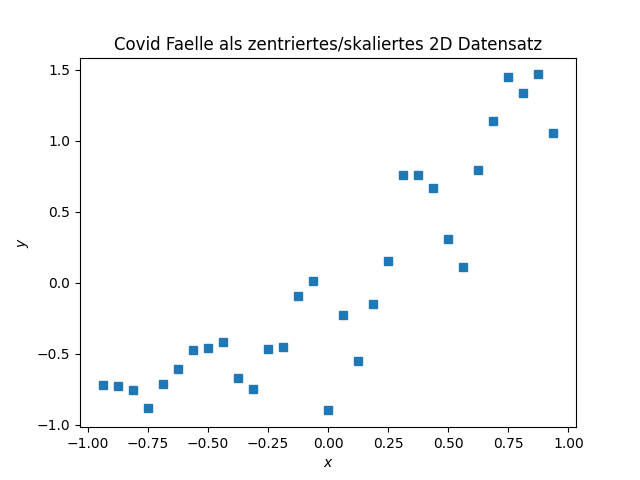
\includegraphics[width=0.65\textwidth,height=\textheight]{bilder/04-covid-cntrd.png}
\caption{Fallzahlen von Sars-CoV-2 in Bayern im Oktober
2020 -- zentriert}\label{fig:cases-cntrd}
}
\end{figure}

\hypertarget{variationskoeffizienten}{%
\section{Variationskoeffizienten}\label{variationskoeffizienten}}

Als nächstes kann Jan sich fragen, wie gut die Daten durch ihren Mittelwert beschrieben werden und die Varianzen berechnen, die für zentrierte Daten so aussehen

\begin{equation*}
s_x^2 = \frac {1}{N-1} \sum_{i=1}^N x_i^2,
\quad
s_y^2 = \frac {1}{N-1} \sum_{i=1}^N y_i^2.
\end{equation*}

Im gegebenen Fall bekommen wir
\begin{equation*}
s_x^2 \approx 0.32
\quad
s_y^2 \approx  0.57
\end{equation*}
und schließen daraus, dass in \(y\) Richtung \emph{viel passiert} und in \(x\) Richtung \emph{nicht ganz so viel}. Das ist jeder Hinsicht nicht befriedigend, wir können weder

\begin{itemize}
\tightlist
\item
  Redundanzen ausmachen (eine Dimension der Daten vielleicht weniger wichtig?) noch
\item
  dominierende Richtungen feststellen (obwohl dem Bild nach so eine offenbar existiert)
\end{itemize}

und müssen konstatieren, dass die Repräsentation der Daten im \((x,y)\) Koordinatensystem nicht optimal ist.

Die Frage ist also, ob es ein Koordinatensystem gibt, dass die Daten besser darstellt.

\leavevmode\hypertarget{rem-coors}{}%
\begin{JHSAYS}
Ein Koordinatensystem ist nichts anderes als eine Basis. Und die Koordinaten eines Datenpunktes sind die Komponenten des entsprechenden Vektors in dieser Basis. Typischerweise sind Koordinatensysteme orthogonal (das heißt eine Orthogonalbasis) und häufig noch orientiert (die Basisvektoren haben eine bestimmte Reihenfolge und eine bestimmte Richtung).

\end{JHSAYS}

\hypertarget{koordinatenwechsel}{%
\section{Koordinatenwechsel}\label{koordinatenwechsel}}

Sei nun also \(\{b_1,b_2\}\subset \mathbb R^{2}\) eine orthogonale Basis.

\leavevmode\hypertarget{rem-ortho-bas}{}%
\begin{JHSAYS}
Wie allgemein gebräuchlich, sagen wir \emph{orthogonal}, meinen aber \emph{orthonormal}. In jedem Falle soll gelten
\begin{equation*}
b_1^T b_1=1, \quad b_2^Tb_2=1, \quad b_1^Tb_2 = b_2^Tb_1 = 0.
\end{equation*}

\end{JHSAYS}

Wir können also alle Datenpunkte
\(\mathbf x_i = \begin{bmatrix} x_i \\ y_i \end{bmatrix}\)
in der neuen Basis darstellen mit eindeutig bestimmten Koeffizienten \(\alpha_{i1}\) und \(\alpha_{i2}\) mittels
\begin{equation*}
\mathbf x_i = \alpha_{i1}b_1 + \alpha_{i2}b_2.
\end{equation*}
Für orthogonale Basen sind die Koeffizienten durch \emph{testen} mit dem Basisvektor einfach zu berechnen:
\begin{align*}
b_1^T\mathbb x_i = b_1^T(\alpha_{i1}b_1 + \alpha_{i2}b_2) = \alpha_{i1}b_1^Tb_1 + \alpha_{i2}b_1^Tb_2 = \alpha_{i1}\cdot 1 + \alpha_{i2} \cdot 0 = \alpha_{i1},\\
b_2^T\mathbb x_i = b_2^T(\alpha_{i1}b_1 + \alpha_{i2}b_2) = \alpha_{i1}b_1^Tb_2 + \alpha_{i2}b_2^Tb_2 = \alpha_{i1}\cdot 0 + \alpha_{i2}\cdot 1 = \alpha_{i2}.
\end{align*}
Es gilt also
\begin{equation*}
\alpha_{i1} = b_1^T\mathbb x = b_1^T\begin{bmatrix}
x_i \\ y_i
\end{bmatrix}, \quad
\alpha_{i2} = b_2^T\mathbb x = b_2^T\begin{bmatrix}
x_i \\ y_i
\end{bmatrix}.
\end{equation*}

Damit, können wir jeden Datenpunkt \(\mathbf x_i=(x_i, y_i)\) in den neuen Koordinaten \((\alpha_{i1}, \alpha_{i2})\) ausdrücken.

Zunächst halten wir fest, dass auch in den neuen Koordinaten die Daten zentriert sind. Es gilt nämlich, dass
\begin{align*}
\frac 1N \sum_{i=1}^N \alpha_{ji}=\frac 1N \sum_{i=1}^N b_j^T\mathbb x_i 
=\frac 1N b_j^T \sum_{i=1}^N \begin{bmatrix} x_i \\ y_i \end{bmatrix}
=& \frac 1N b_j^T \begin{bmatrix} \sum_{i=1}^N x_i \\ \sum_{i=1}^N y_i \end{bmatrix}\\
&=b_j^T \begin{bmatrix} \frac 1N \sum_{i=1}^N x_i \\ \frac 1N \sum_{i=1}^N y_i \end{bmatrix}
=b_j^T \begin{bmatrix} 0 \\ 0 \end{bmatrix} = 0,
\end{align*}
für \(j=1,2\).

Desweiteren gilt wegen der Orthogonalität von \(B=[b_1~b_2]\in \mathbb R^{2\times 2}\), dass
\begin{equation*}
x_{i}^2 + y_{i}^2 = \|\mathbb x_i\|^2 = \|B^T\mathbb x_i\|^2 
= \|\begin{bmatrix} b_1^T \\ b_2^T \end{bmatrix} \mathbb x_i\|^2
= \|\begin{bmatrix} b_1^T\mathbb x \\ b_2^T\mathbb x \end{bmatrix}\|^2
= \|\begin{bmatrix} \alpha_{i1} \\ \alpha_{i2} \end{bmatrix}\|^2
= \alpha_{i1}^2 + \alpha_{i2}^2
\end{equation*}
woraus wir folgern, dass in jedem orthogonalen Koordinatensystem, die Summe der beiden Varianzen die gleiche ist:
\begin{equation*}
s_x^2 + s_y^2 = \frac{1}{N-1}\sum_{i=1}^N(x_i^2 + y_i^2) = \frac{1}{N-1}\sum_{i=1}^N(\alpha_{i1}^2 + \alpha_{i2}^2) =: s_1^2 + s_2^2.
\end{equation*}

Das bedeutet, dass durch die Wahl des Koordinatensystems die Varianz als Summe nicht verändert wird. Allerdings können wir das System so wählen, dass eine der Varianzen in Achsenrichtung maximal wird (und die übrige(n) entsprechend klein).

Analog gilt für den eigentlichen Mittelwert der (nichtzentrierten) Daten, dass die Norm gleich bleibt. In der Tat, für die \emph{neuen} Koordinaten des Mittelwerts gilt in der Norm
\begin{equation*}
\|
\begin{bmatrix}
\alpha_{c1} \\ \alpha_{c2}
\end{bmatrix}
\|
=
\|
B^T
\begin{bmatrix}
x_c \\ y_c
\end{bmatrix}
\|
=
\|
\begin{bmatrix}
x_c \\ y_c
\end{bmatrix}
\|.
\end{equation*}

\hypertarget{sec-pca-maximierung}{%
\section{Maximierung der Varianz in (Haupt)-Achsenrichtung}\label{sec-pca-maximierung}}

Wir wollen nun also \(b_1\in \mathbb R^{2}\), mit \(\|b_1\|=1\) so wählen, dass
\begin{equation*}
s_1^2 = \frac{1}{N-1}\sum_{i=1}^n \alpha_{i1}^2
\end{equation*}
maximal wird. Mit der Matrix \(\mathbf X\) aller Daten
\begin{equation*}
\mathbf X = \begin{bmatrix}
x_1 & y_1 \\ x_2 & y_2 \\ \vdots & \vdots \\ x_N & y_N
\end{bmatrix} = 
\begin{bmatrix}
\mathbf x_1^T\\ \mathbf x_2^T  \\  \vdots \\ \mathbf x_N^T
\end{bmatrix} 
\in \mathbb R^{N\times 2}
\end{equation*}
können wir die Varianz in \(b_1\)-Richtung kompakt schreiben als
\begin{equation*}
s_1^2 = \frac{1}{N-1}\sum_{i=1}^n \alpha_{i1}^2
= \frac{1}{N-1}\sum_{i=1}^n (b_1^T\mathbf x_i)^2
= \frac{1}{N-1}\sum_{i=1}^n (\mathbf x_i^Tb_1)^2
= \frac{1}{N-1}\| \mathbf X b_1 \|^2
\end{equation*}
Wir sind also ein weiteres mal bei einem Optimierungsproblem (diesmal mit Nebenbedingung) angelangt:
\begin{equation*}
\max_{b\in \mathbb R^{2},\, \|b\|=1} \|\mathbf X b\|^2
\end{equation*}
Die Lösung dieses Problems ist mit \(b=v_1\) gegeben, wobei \(v_1\) der erste (rechte) Singulärvektor von \(\mathbf X\) ist:
\begin{equation*}
\mathbf X = U \Sigma V^T = U \Sigma \begin{bmatrix}
v_1^T \\ v_2^T
\end{bmatrix}.
\end{equation*}
Und damit rechnen wir auch direkt nach, dass im neuen Koordinatensystem \(\{b_1, b_2\}=\{v_1, v_2\}\) die Varianzen \(s_1^2\) und \(s_2^2\) (bis auf einen Faktor von \(\frac{1}{N-1}\)) genau die quadrierten Singulärwerte von \(\mathbf X\) sind:
\begin{align*}
(N-1)s_1^2 
= \|\mathbf X v_1 \|^2 = \|U \Sigma \begin{bmatrix} v_1^T \\ v_2^T \end{bmatrix}v_1\|^2
= \|\Sigma \begin{bmatrix} v_1^Tv_1 \\ v_2^T v_1\end{bmatrix}\|^2
=  \|\Sigma \begin{bmatrix} 1 \\  0\end{bmatrix}\|^2
=\sigma_1^2,\\
(N-1)s_2^2 
= \|\mathbf X v_2 \|^2 = \|U \Sigma \begin{bmatrix} v_1^T \\ v_2^T \end{bmatrix}v_2\|^2
= \|\Sigma \begin{bmatrix} v_1^Tv_2 \\ v_2^T v_2\end{bmatrix}\|^2
=  \|\Sigma \begin{bmatrix} 0 \\  1\end{bmatrix}\|^2
=\sigma_2^2
\end{align*}

Für unser Covid Beispiel ergibt sich
\begin{equation*}
V^T \approx
\begin{bmatrix}
0.5848 &  0.8111 \\
0.8111 & -0.5848
\end{bmatrix}
\end{equation*}
also
\begin{equation*}
b_1 = v_1 = \begin{bmatrix}
0.5848 \\  0.8111 
\end{bmatrix}
\quad
b_2 = v_2 = \begin{bmatrix}
0.8111 \\ -0.5848
\end{bmatrix}
\end{equation*}
als neue Koordinatenrichtungen mit
\begin{equation*}
s_1^2 \approx 0.85, \quad s_2^2 \approx 0.04,
\end{equation*}
was bereits eine deutliche Dominanz der \(v_1\)-Richtung -- genannt \emph{Hauptachse} -- zeigt.

Im Hinblick auf die nächste Vorlesung, in der wir Anwendungen und Eigenschaften der PCA untersuchen werden, noch ein Plot der Daten mit der \(v_1\)-Richtung als Linie eingezeichnet.

\begin{figure}
\hypertarget{fig:cases-cntrd-HA}{%
\centering
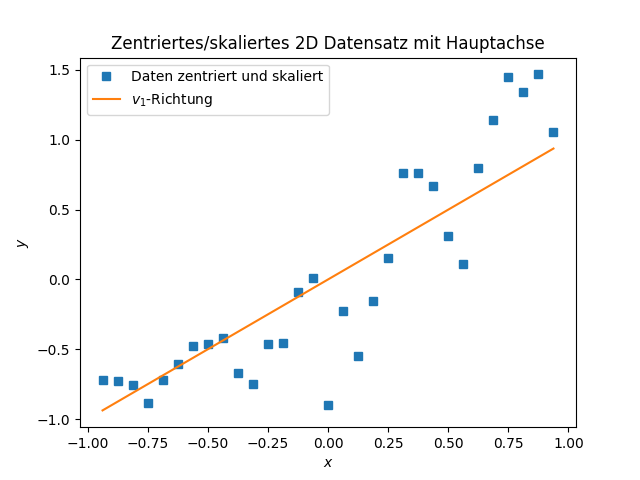
\includegraphics[width=0.65\textwidth,height=\textheight]{bilder/04-covid-cntrd-HA.png}
\caption{Fallzahlen von Sars-CoV-2 in Bayern im Oktober
2020 -- zentriert/skaliert/Hauptachse}\label{fig:cases-cntrd-HA}
}
\end{figure}

\hypertarget{hauptkomponentenanalyse-ctd.}{%
\chapter{Hauptkomponentenanalyse Ctd.}\label{hauptkomponentenanalyse-ctd.}}

\newcommand{\Cov}{\operatorname{Cov}}
\newcommand{\bX}{{\mathbf{X}}}
\newcommand{\bxi}{{\mathbf{x} _ i}}
\newcommand{\bxj}{{\mathbf{x} _ j}}
\newcommand{\bxixj}{{\mathbf{x} _ i \mathbf{x} _ j}}

Im vorherigen Kapitel hatten wir einen zweidimensionalen Datensatz betrachtet und dafür die Richtung bestimmt, in der die Varianz maximal wird.
Da wir außerdem ermittelt hatten, dass die Summe der Varianz unabhüngig vom Koordinatensystem ist (es muss nur ein orthogonales sein) bedeutete das gleichzeitig, dass die verbleibende Richtung die Richtung der minimalen Varianz war.

Jetzt wollen wir einen Datensatz mit mehr Merkmalen betrachten und sehen, wie die algorithmische Herangehensweise zum Verständnis beiträgt.

\hypertarget{der-penguins-datensatz}{%
\section{Der PENGUINS Datensatz}\label{der-penguins-datensatz}}

Die Grundlage ist der \href{https://allisonhorst.github.io/palmerpenguins/}{\emph{Pinguin Datensatz}}, der eine gern genommene Grundlage für die Illustration in der Datenanalyse ist. Die Daten wurden von \href{https://www.uaf.edu/cfos/people/faculty/detail/kristen-gorman.php}{Kristen Gorman} erhoben und beinhalten 4 verschiedene Merkmale (engl. \emph{features}) von einer Stichprobe von insgesamt 344\footnote{allerdings mit 2 unvollständigen Datenpunkten, die ich entfernt habe für unseere Beispiele}Pinguinen die 3 verschiedenen Spezies zugeordnet werden können oder sollen (Fachbegriff hier: \emph{targets}). Im Beispiel werden die Klassen mit \texttt{0,\ 1,\ 2} codiert und beschreiben die Unterarten \emph{Adele}, \emph{Gentoo} und \emph{Chinstrap} der Pinguine. Die Merkmale sind gemessene Länge und Höhe des Schnabels (hier \emph{bill}), die Länge der Flosse (\emph{flipper}) sowie das Köpergewicht\footnote{Im Originaldatensatz ist das Gewicht in Gramm angegeben, um die Daten innerhalb einer 10er Skala zu haben, habe ich das Gewicht auf in kg umgerechnet}
(\emph{body mass}).

Wir stellen uns 2-3 Fragen:

\begin{enumerate}
\def\labelenumi{\arabic{enumi}.}
\tightlist
\item
  Würden eventuell 3 (oder sogar nur 2) Dimensionen reichen um den Datensatz zu beschreiben?
\item
  Können wir aus den Merkmalen (\emph{features}) die Klasse (\emph{target}) erkennen und wie machen wir gegebenenfalls die Zuordnung?
\end{enumerate}

\hypertarget{darstellung}{%
\section{Darstellung}\label{darstellung}}

In höheren Dimensionen ist schon die graphische Darstellung der Daten ein Problem. Wir können aber alle möglichen 2er Kombinationen der Daten in 2D plots visualisieren.

\begin{figure}
\hypertarget{fig:05-penguin-allpairs}{%
\centering
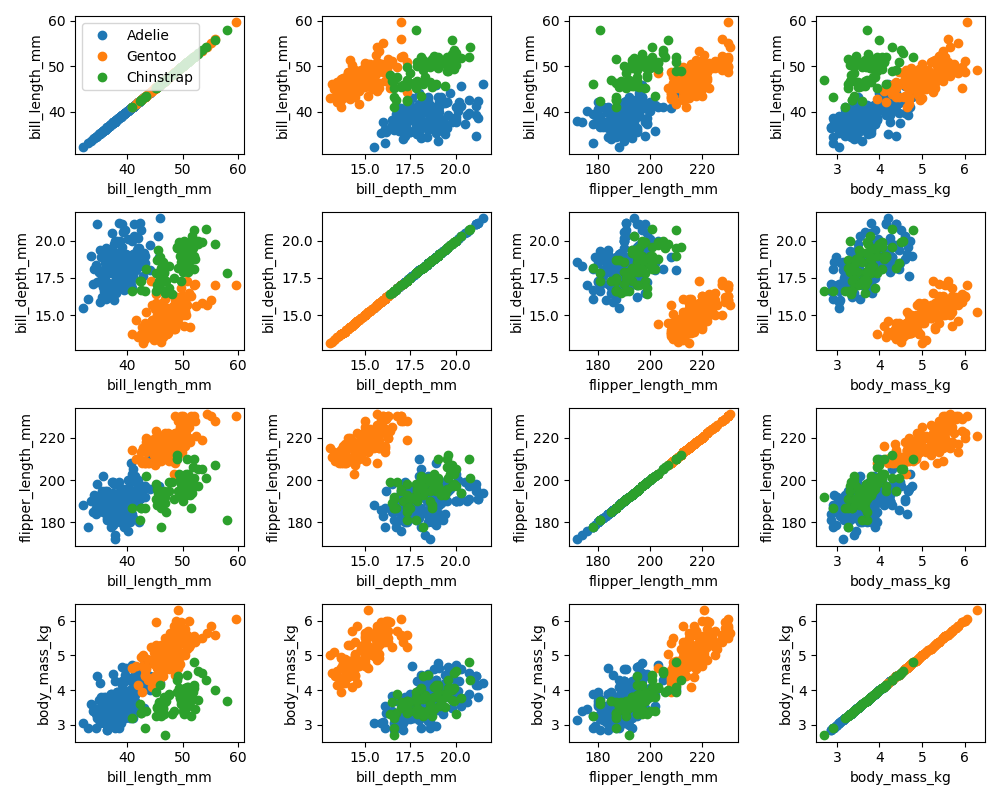
\includegraphics[width=0.75\textwidth,height=\textheight]{bilder/05-all-pairs.png}
\caption{Pinguin Datenset 2D plots}\label{fig:05-penguin-allpairs}
}
\end{figure}

Ein Blick auf die Diagonale zeigt schon, dass manche Merkmale besser geeignet als andere sind, um die Spezies zu unterscheiden, allerdings keine der Zweierkombinationen eine Eindeutige Diskriminierung erlaubt.

\hypertarget{korrelationen-und-die-kovarianzmatrix}{%
\section{Korrelationen und die Kovarianzmatrix}\label{korrelationen-und-die-kovarianzmatrix}}

Als nächstes suchen wir nach Korrelationen in den Daten in dem wir für alle Merkmalpaare die Korrelationen ausrechnen. Dafür berechnen wir die sogenannte \emph{Kovarianzmatrix}
\begin{equation*}
\operatorname{Cov}(\mathbf X) = \begin{bmatrix}
\rho_{{\mathbf{x} _ i \mathbf{x} _ j}}
\end{bmatrix}_{i,j=1,\dots n} \in \mathbb R^{n\times n}
\end{equation*}
wobei \(n\) die Dimension der Daten ist und wobei
\begin{equation*}
s_{{\mathbf{x} _ i \mathbf{x} _ j}} = \frac{1}{N-1} \sum_{k=1}^N (x_{ik}-\overline{{\mathbf{x} _ i}})(x_{jk}-\overline{{\mathbf{x} _ j}} ).
\end{equation*}
die Kovarianzen sind, die wir auch schon in der ersten Vorlesung kennengelernt haben.

Ist \(\mathbf X\in \mathbb R^{N\times n}\) die Matrix mit den Datenvektoren \({\mathbf{x} _ i}\in \mathbb R^{n}\) als Spalten \textbf{und ist der Datensatz zentriert} so erhalten wir die Kovarianzmatrix als
\begin{equation*}
\operatorname{Cov}({\mathbf{X}}) = \frac{1}{N-1}{\mathbf{X}}^T {\mathbf{X}}
\end{equation*}

Wir bemerken, dass auf der Hauptdiagonalen die Varianzen in Koordinatenrichtung stehen und in den Zeilen oder Spalten ein Mass dafür, wie bspw. \({\mathbf{x} _ i}\) und \({\mathbf{x} _ j}\) korreliert sind. Große Zahlen bedeuten eine große Varianz oder eine starke Korrelation und umgekehrt. Für die Datenanalyse können wir \(\operatorname{Cov}({\mathbf{X}})\) wie folgt heranziehen:

\hypertarget{hauptachsentransformation}{%
\section{Hauptachsentransformation}\label{hauptachsentransformation}}

Wie im vorherigen Kapitel hergeleitet, bedeutet ein Koordinatenwechsel die Multiplikation der Datenmatrix \({\mathbf{X}}\in \mathbb R^{N\times n}\) mit einer orthogonalen
Matrix \(V\in \mathbb R^{n\times n}\):
\begin{equation*}
\tilde {\mathbf{X}}= {\mathbf{X}}V,
\end{equation*}
wobei \(\tilde {\mathbf{X}}\) die Daten in den neuen Koordinaten sind (die Basisvektoren sind dann die Zeilenvektoren von \(V\)). Wir wollen nun eine Basis finden, in der

\begin{itemize}
\tightlist
\item
  \(\operatorname{Cov}({\mathbf{X}})\) eine Diagonalmatrix ist --- damit wären alle Richtungen in den Daten \emph{unkorreliert} und könnten \emph{unabhängig} voneinander betrachtet werden\footnote{wir dürfen aber nicht vergessen, dass Daten typischerweise nur eine Stichprobe von Beobachtungen eines Phänomens sind. Die Unabhängigkeit in den \emph{features} gilt also nur für die gesammelten Daten aber in der Regel nicht für das Phänomen. Für normalverteilte Prozesse liefern die daten-basiert ermittelten Hauptrichtungen jedoch auch die Hauptrichtungen des zugrundeliegenden Phänomens} --
\item
  und in der die neuen Varianzen nach Größe geordnet sind gleichzeitig die verfügbare Varianz maximal in wenigen Richtungen konzentrieren.
\end{itemize}

Nachden den Überlegungen im vorherigen Kapitel ist die erste Hauptrichtung durch den ersten rechten Singulärvektor \(v_1\in \mathbb R^{n}\) der (\emph{ökonomischen}) Singulärwertzerlegung
\begin{equation*}
{\mathbf{X}}= U\Sigma V^* = 
\begin{bmatrix}
u_1 & u_2 & \dots & u_n
\end{bmatrix}
\begin{bmatrix}
\sigma_1 \\ &\sigma_2 \\ &&\ddots \\ &&&\sigma_n
\end{bmatrix}
\begin{bmatrix}
v_1^* \\ v_2 ^* \\ \vdots \\ v_n^*
\end{bmatrix}
\end{equation*}
von \(\mathbf X\in \mathbb R^{N\times n}\) gegeben. Die zugehörigen Koeffizenten berechnen wir mittels
\begin{equation*}
\tilde {\mathbf{X}}= {\mathbf{X}}v_1.
\end{equation*}

\hypertarget{rekonstruktion}{%
\section{Rekonstruktion}\label{rekonstruktion}}

Um zu plausibilisieren, dass die weiteren Hauptachsen durch die weiteren (rechten) Singulärvektoren gegeben sind, betrachten wir erst die \emph{Rekonstruktion}
also die Darstellung im Ausgangskoordinatensystem (mit den messbaren oder interpretierbaren Features) die durch
\begin{equation*}
\tilde {\tilde {\mathbf{X}}} = {\mathbf{X}}v_1v_1^T
\end{equation*}
gegeben ist.
Die letzte Formel wird vielleicht klarer, wenn Jan sich überlegt, dass für einen Datenpunkt \({\mathbf{X}}_j=\begin{bmatrix} x_{1j} &x_{2j} & \dots& x_{nj}\end{bmatrix}\) (also die \(j\)-te Zeile von \({\mathbf{X}}\)), der Koeffizient für \(v_1\) gegeben ist durch \(\alpha_j=v_1^T{\mathbf{X}}_j^T\) und die Darstellung im Vektorraum durch
\begin{equation*}
\tilde{\tilde{ {\mathbf{X}}}}_j=(\alpha_j v_1)^T = \alpha_j v_1^T = (v_1^T {\mathbf{X}}_j^T) v_1^T  = {\mathbf{X}}_j  v_1 v_1^T
\end{equation*}
gegeben ist.

Damit können wir mit
\begin{equation*}
{\mathbf{X}}- \tilde{\tilde {{\mathbf{X}}}} = {\mathbf{X}}(I-v_1v_1^T)
\end{equation*}
den Teil der Daten betrachten, der durch die Richtung \(v_1\) nicht abgebildet wird (sozusagen den noch verbleibenden Teil). Jan kann nachrechnen, dass wiederum \(U\) und \(V\) die Singulärvektoren von \({\mathbf{X}}-\tilde{\tilde {{\mathbf{X}}}}\) bilden, mit jetzt \(v_2\) als Richtung mit dem größten (verbleibenden) Singulärwert.

Das heißt, dass der \(k\)-te Singulärvektor die \(k\)-te Hauptrichtung bildet.

\hypertarget{reduktion-der-daten}{%
\section{Reduktion der Daten}\label{reduktion-der-daten}}

Ist die Datenmatrix mit linear abhängigen Spalten besetzt, äußert sich das in \(\sigma_k = 0\) für ein \(k<n\) (und alle noch folgenden Singulärwerte). Jan rechnet nach, dass dann
\begin{equation*}
{\mathbf{X}}= {\mathbf{X}}V_{k-1}V_{k-1}^T
\end{equation*}
wobei \(V_{k-1}\) die Matrix der \(k-1\) führenden Singulärvektoren ist und das entsprechende
\begin{equation*}
\tilde {\mathbf{X}}= {\mathbf{X}}V_{k-1}
\end{equation*}
alle Informationen des Datensatzes in kleinerer Dimension parametrisiert.

In der Praxis sind schon allein durch Messfehler exakte lineare Abhängigkeiten sowie durch die näherungsweise Bestimmung auf dem Computer das Auftreten von \(\sigma_k =0\) quasi ausgeschlossen. Stattdessen werden Schwellwerte definiert, unterhalb derer die SVD abgeschnitten wird.

Wie oben, werden dann die Daten \(\tilde {\mathbf{X}}={\mathbf{X}}V_{\hat k}\) in den (reduzierten) Koordinaten der Hauptachsen betrachtet sowie die Rekonstruktion \(\hat {\mathbf{X}}= {\mathbf{X}}V_{\hat k}V_{\hat k}^T\), wobei der \(V_{\hat k}\) die Matrix der \(\hat k\) führenden Singulärvektoren sind (mit Singulärwerten überhalb des Schwellwertes).

\hypertarget{am-beispiel-der-pinguin-daten}{%
\section{Am Beispiel der Pinguin Daten}\label{am-beispiel-der-pinguin-daten}}

Wir stellen die Daten noch einmal zentriert dar:

\begin{figure}

{\centering 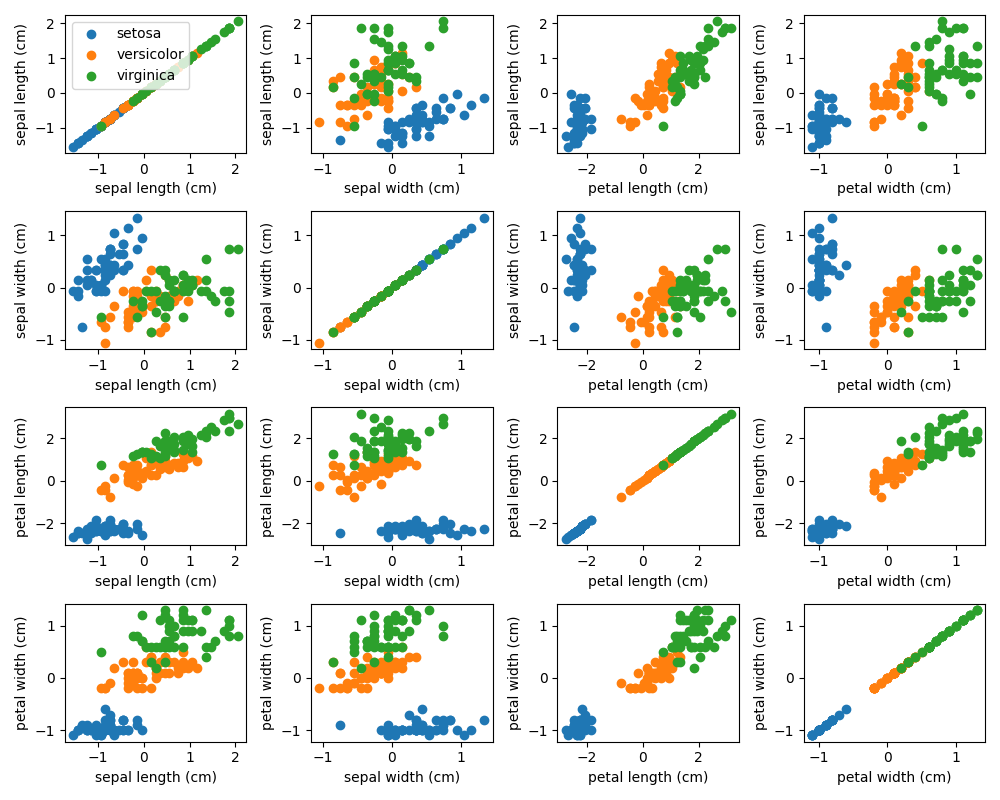
\includegraphics[width=0.75\linewidth]{bilder/05-all-pairs-cntrd} 

}

\caption{Pinguin Daten Zentriert}\label{fig:05-penguin-allpairs-cntrd}
\end{figure}

Für die Kovarianzmatrix der Pinguin Daten erhalten wir:

\begin{Shaded}
\begin{Highlighting}[]
\NormalTok{Covariance matrix: }
\NormalTok{[[ }\FloatTok{29.8071}  \OperatorTok{{-}}\FloatTok{2.5342}  \FloatTok{50.3758}   \FloatTok{2.6056}\NormalTok{]}
\NormalTok{ [ }\OperatorTok{{-}}\FloatTok{2.5342}   \FloatTok{3.8998} \OperatorTok{{-}}\FloatTok{16.213}   \OperatorTok{{-}}\FloatTok{0.7474}\NormalTok{]}
\NormalTok{ [ }\FloatTok{50.3758} \OperatorTok{{-}}\FloatTok{16.213}  \FloatTok{197.7318}   \FloatTok{9.8244}\NormalTok{]}
\NormalTok{ [  }\FloatTok{2.6056}  \OperatorTok{{-}}\FloatTok{0.7474}   \FloatTok{9.8244}   \FloatTok{0.6431}\NormalTok{]]}
\end{Highlighting}
\end{Shaded}

Für die Singulärwerte:

\begin{Shaded}
\begin{Highlighting}[]
\NormalTok{In: U, S, Vh }\OperatorTok{=}\NormalTok{ np.linalg.svd(data, full\_matrices}\OperatorTok{=}\VariableTok{False}\NormalTok{)}

\NormalTok{In: }\BuiltInTok{print}\NormalTok{(S)}
\NormalTok{Out: [}\FloatTok{269.7858}  \FloatTok{74.1334}  \FloatTok{28.4183}   \FloatTok{7.2219}\NormalTok{]}
\end{Highlighting}
\end{Shaded}

Zwar ist hier kein Singulärwert nah an der Null, allerdings beträgt der Unterschied zwischen dem größten und dem kleinsten schon eine gute 10er Potenz, was auf eine starke Dominanz der ersten Hauptachsen hinweist.

In der Tat, plotten wir die Daten in den Koordinaten der Hauptachsen (also \(\tilde {\mathbf{X}}\)), zeigen Bilder der \(v_1\) oder \(v_2\)-Koordinaten klare Tendenzen in den Daten, während die Plots der übrigen Richtungen wie eine zufällige Punktwolke aussieht, vgl. die Abbildung \protect\hyperlink{fig:05-penguin-allpairs-pcs}{hier}.

\begin{figure}
\hypertarget{fig:05-penguin-allpairs-pcs}{%
\centering
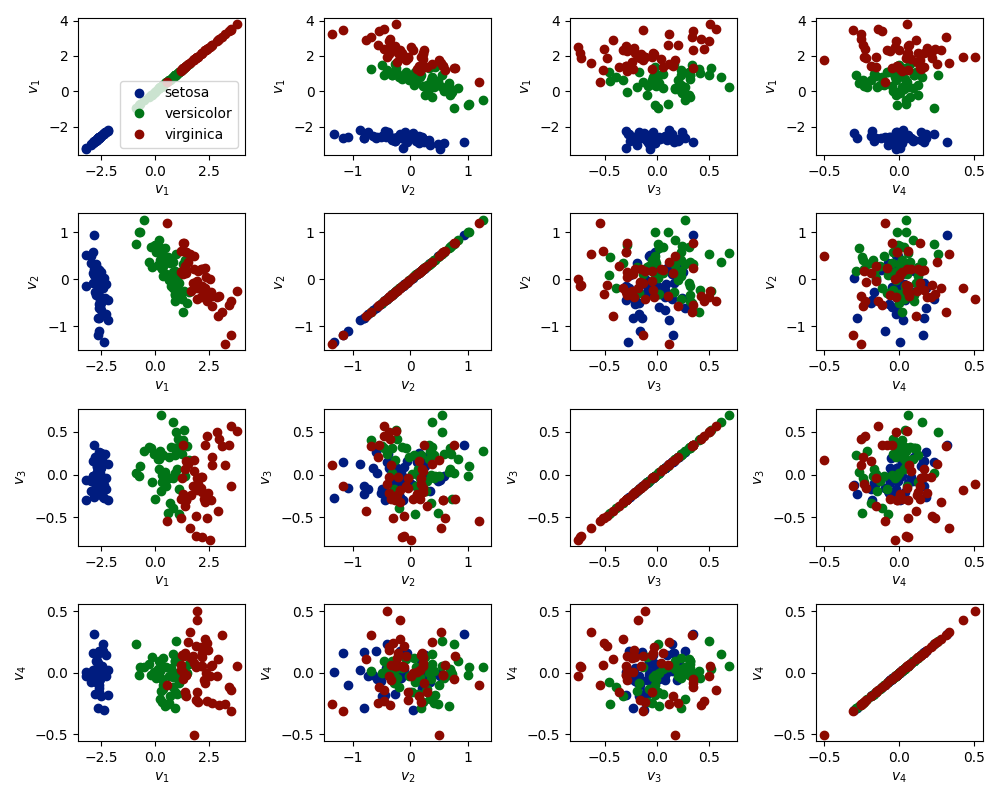
\includegraphics[width=0.75\textwidth,height=\textheight]{bilder/05-all-pairs-pcs.png}
\caption{Pinguin Datenset 2D plots in Hauptachsenkoordinaten}\label{fig:05-penguin-allpairs-pcs}
}
\end{figure}

Als letztes plotten wir noch \(\hat {{\mathbf{X}}}\) für \(\hat k =2\). Das heißt wir reduzieren die Daten auf die \(v_1\) und \(v_2\)-Richtungen und betrachten die Rekonstruktion. Im Plot sehen wir, dass in gewissen Teilen die Daten gut rekonstruiert werden. Allerdings, hat \(\hat{{\mathbf{X}}}\) nur Rang \(\operatorname{Rk} \hat {{\mathbf{X}}}=2\) (warum?), sodass in den Plots notwendigerweise direkte lineare Abhängigkeiten offenbar werden.

\begin{figure}
\hypertarget{fig:05-penguin-allpairs-k2-rec}{%
\centering
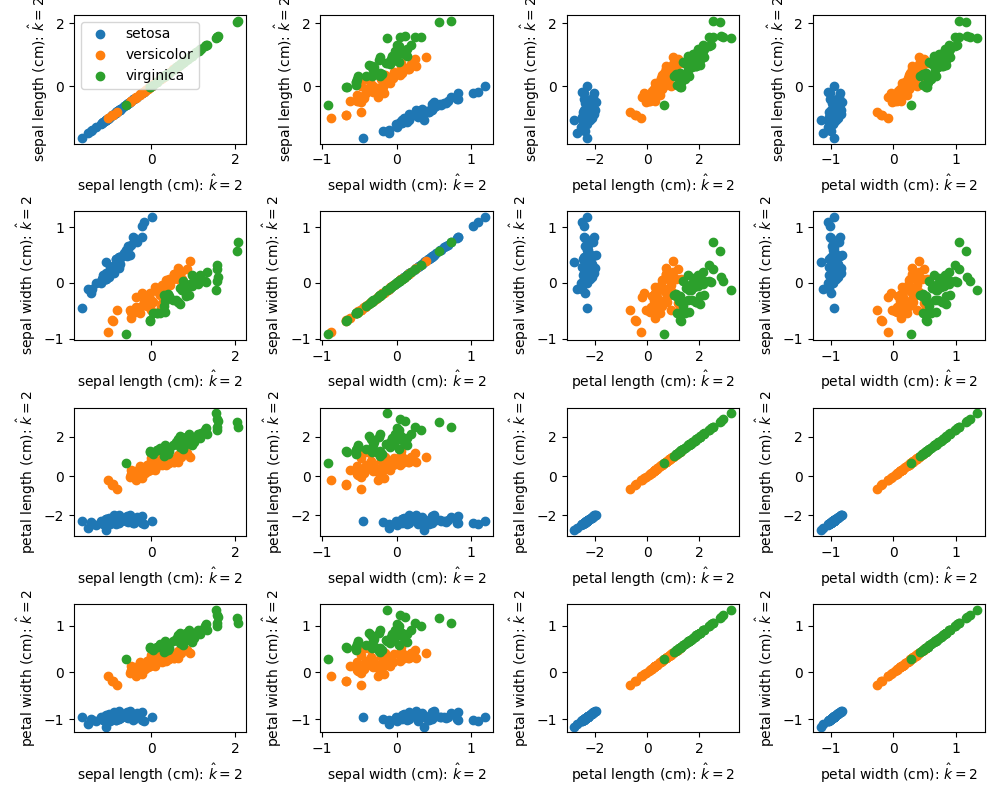
\includegraphics[width=0.75\textwidth,height=\textheight]{bilder/05-all-pairs-k2-rec.png}
\caption{Pinguin Datenset -- rekonstruiert von \(\hat k =2\) Hauptachsenkoordinaten}\label{fig:05-penguin-allpairs-k2-rec}
}
\end{figure}

\hypertarget{aufgaben-2}{%
\section{Aufgaben}\label{aufgaben-2}}

\hypertarget{kovarianzen-pt}{%
\subsection{Kovarianzen (P+T)}\label{kovarianzen-pt}}

Erzeugen Sie für \texttt{N} aus \texttt{Nl\ =\ {[}10,\ 1000,\ 100000{]}} zufällige Vektoren \texttt{x} und \texttt{y} der Länge \texttt{N} und berechnen Sie
für den Datensatz \texttt{X\ =\ {[}x,\ x,\ x*y,\ y{]}}
jeweils die Matrix der Korrelationskoeffizienten
\begin{equation*}
\rho _{i\;j} = \frac{s_{i\, j}}{s_i \cdot s_j}
\end{equation*}
wobei \(s_{i\,j}\) die Kovarianz der Daten \({\mathbf{x} _ i}\) und \({\mathbf{x} _ j}\) ist und \(s_{i}\) die Varianz von \({\mathbf{x} _ i}\). Interpretieren sie die Ergebnisse.

\textbf{Hinweis}: Weil Zufälligkeit involviert ist, ist die Interpretation manchmal schwierig. Lassen sie das Programm öfter laufen und beobachten sie verschiedene Realisierungen der Stichproben.

\begin{Shaded}
\begin{Highlighting}[]
\ImportTok{import}\NormalTok{ numpy }\ImportTok{as}\NormalTok{ np}

\CommentTok{\# N = 10}

\NormalTok{x }\OperatorTok{=}\NormalTok{ np.random.randn(}\DecValTok{10}\NormalTok{, }\DecValTok{1}\NormalTok{)}
\NormalTok{y }\OperatorTok{=}\NormalTok{ np.random.randn(}\DecValTok{10}\NormalTok{, }\DecValTok{1}\NormalTok{)}

\NormalTok{X }\OperatorTok{=}\NormalTok{ np.hstack([x, x, x}\OperatorTok{*}\NormalTok{y, y])}

\NormalTok{Xcntrd }\OperatorTok{=}\NormalTok{ X }\OperatorTok{{-}}\NormalTok{ X.mean(axis}\OperatorTok{=}\DecValTok{0}\NormalTok{)}
\CommentTok{\# zentrieren der Daten}

\CommentTok{\# Kovarianz Matrix ausrechnen}
\NormalTok{covX }\OperatorTok{=} \DecValTok{1}\OperatorTok{/}\NormalTok{(}\DecValTok{10}\OperatorTok{{-}}\DecValTok{1}\NormalTok{)}\OperatorTok{*}\NormalTok{Xcntrd.T }\OperatorTok{@}\NormalTok{ Xcntrd}

\CommentTok{\# Varianzen {-}{-} stehen auf der Diagonalen im Quadrat}
\NormalTok{varvec }\OperatorTok{=}\NormalTok{ np.sqrt(np.diagonal(covX)).reshape(}\DecValTok{4}\NormalTok{, }\DecValTok{1}\NormalTok{)}
\CommentTok{\# Matrix mit den Kombinationen aller Varianzen}
\NormalTok{varmat }\OperatorTok{=}\NormalTok{ varvec }\OperatorTok{@}\NormalTok{ varvec.T}

\NormalTok{matcc }\OperatorTok{=}\NormalTok{ covX }\OperatorTok{*} \DecValTok{1}\OperatorTok{/}\NormalTok{varmat}

\BuiltInTok{print}\NormalTok{(}\SpecialStringTok{f\textquotesingle{}N=}\SpecialCharTok{\{}\DecValTok{10}\SpecialCharTok{\}}\SpecialStringTok{ : Matrix of Correlation Coefficients=\textquotesingle{}}\NormalTok{)}
\BuiltInTok{print}\NormalTok{(matcc)}
\end{Highlighting}
\end{Shaded}

\hypertarget{pinguin-datensatz-targets-plotten-p}{%
\subsection{Pinguin Datensatz -- Targets Plotten (P)}\label{pinguin-datensatz-targets-plotten-p}}

Laden Sie die \href{bilder/penguin-data.json}{Pinguin Datensatz} (hier als \texttt{json} file bereitgestellt) und plotten sie \texttt{bill\_length} versus \texttt{flipper\_length} für die drei Spezies \texttt{Adelie}, \texttt{Gentoo}, \texttt{Chinstrap} in drei separaten Grafiken.

\begin{Shaded}
\begin{Highlighting}[]
\ImportTok{import}\NormalTok{ json}

\ImportTok{import}\NormalTok{ numpy }\ImportTok{as}\NormalTok{ np}
\ImportTok{import}\NormalTok{ matplotlib.pyplot }\ImportTok{as}\NormalTok{ plt}

\ControlFlowTok{with} \BuiltInTok{open}\NormalTok{(}\StringTok{\textquotesingle{}penguin{-}data.json\textquotesingle{}}\NormalTok{, }\StringTok{\textquotesingle{}r\textquotesingle{}}\NormalTok{) }\ImportTok{as}\NormalTok{ f:}
\NormalTok{    datadict }\OperatorTok{=}\NormalTok{ json.load(f)}

\BuiltInTok{print}\NormalTok{(datadict.keys())}

\NormalTok{data }\OperatorTok{=}\NormalTok{ np.array(datadict[}\StringTok{\textquotesingle{}data\textquotesingle{}}\NormalTok{])}
\NormalTok{target }\OperatorTok{=}\NormalTok{ np.array(datadict[}\StringTok{\textquotesingle{}target\textquotesingle{}}\NormalTok{])}
\NormalTok{feature\_names }\OperatorTok{=}\NormalTok{ datadict[}\StringTok{\textquotesingle{}feature\_names\textquotesingle{}}\NormalTok{]}
\NormalTok{target\_names }\OperatorTok{=}\NormalTok{ datadict[}\StringTok{\textquotesingle{}target\_names\textquotesingle{}}\NormalTok{]}

\BuiltInTok{print}\NormalTok{(}\StringTok{\textquotesingle{}target names: \textquotesingle{}}\NormalTok{, target\_names)}
\BuiltInTok{print}\NormalTok{(}\StringTok{\textquotesingle{}feature names: \textquotesingle{}}\NormalTok{, feature\_names)}

\NormalTok{fig, axs }\OperatorTok{=}\NormalTok{ plt.subplots(nrows}\OperatorTok{=}\DecValTok{1}\NormalTok{, ncols}\OperatorTok{=}\DecValTok{3}\NormalTok{, figsize}\OperatorTok{=}\NormalTok{(}\DecValTok{10}\NormalTok{, }\DecValTok{3}\NormalTok{))}

\CommentTok{\# \# Ein Vektor der aus dem Target Vektor das target 0 raussucht}
\NormalTok{trgtidx\_z }\OperatorTok{=}\NormalTok{ (target }\OperatorTok{==} \DecValTok{0}\NormalTok{)}
\CommentTok{\# \# Wird gleich benutzt um die Daten nach diesem target zu filtern}

\NormalTok{target\_z\_daten }\OperatorTok{=}\NormalTok{ data[trgtidx\_z, :]}

\NormalTok{axs[}\DecValTok{0}\NormalTok{].plot(target\_z\_daten[:, }\DecValTok{2}\NormalTok{], target\_z\_daten[:, }\DecValTok{0}\NormalTok{],}
            \StringTok{\textquotesingle{}o\textquotesingle{}}\NormalTok{, label}\OperatorTok{=}\NormalTok{target\_names[}\DecValTok{0}\NormalTok{])}

\NormalTok{axs[}\DecValTok{0}\NormalTok{].legend()}
\NormalTok{axs[}\DecValTok{0}\NormalTok{].set\_xlabel(feature\_names[}\DecValTok{3}\NormalTok{])}
\NormalTok{axs[}\DecValTok{0}\NormalTok{].set\_ylabel(feature\_names[}\DecValTok{0}\NormalTok{])}
\NormalTok{axs[}\DecValTok{0}\NormalTok{].set\_title(target\_names[}\DecValTok{0}\NormalTok{])}

\NormalTok{plt.tight\_layout()}
\NormalTok{plt.show()}
\end{Highlighting}
\end{Shaded}

Hier wurden die \texttt{python} Datentypen

\begin{itemize}
\tightlist
\item
  \emph{list} -- z.B. \texttt{datenpunkte\ =\ {[}1,\ 2,\ 3{]}}
\item
  \emph{array} -- z.B. \texttt{datenmatrix\ =\ np.array(datenpunkte)}
\item
  \emph{dictionary} -- z.B. \texttt{datadict\ =\ \{\textquotesingle{}data\textquotesingle{}:\ datenpunkte\}}
\end{itemize}

verwendet, die alle für verschiedene Zwecke gerne benutzt werden. Z.B.

\begin{itemize}
\tightlist
\item
  Liste -- als eine Sammlung von (möglicherweise total unterschiedlichen) Objekten, über die iteriert werden kann und die einfach zu erweitern ist
\item
  \texttt{arrays} -- Matrix/Vektor von Daten eines Typs, mit denen \emph{gerechnet} werden kann
\item
  \texttt{dictionaries} -- ein \emph{Lookup table}. Objekte können über einen Namen addressiert werden. Ich nehme sie gerne um Daten mit ihrem Namen zum Beispiel als \texttt{json} file zu speichern.
\end{itemize}

\hypertarget{pinguin-datensatz-2d-plots-p}{%
\subsection{Pinguin Datensatz -- 2D plots (P)}\label{pinguin-datensatz-2d-plots-p}}

Erzeugen sie die \protect\hyperlink{fig:05-penguin-allpairs}{Abbildung aller Merkmalpaare} zum Beispiel über ein \texttt{4x4} Feld von subplots

\begin{Shaded}
\begin{Highlighting}[]
\NormalTok{fig, axs }\OperatorTok{=}\NormalTok{ plt.subplots(nrows}\OperatorTok{=}\DecValTok{4}\NormalTok{, ncols}\OperatorTok{=}\DecValTok{4}\NormalTok{, figsize}\OperatorTok{=}\NormalTok{(}\DecValTok{10}\NormalTok{, }\DecValTok{8}\NormalTok{))}
\end{Highlighting}
\end{Shaded}

erzeugen, in das sie mittels

\begin{Shaded}
\begin{Highlighting}[]
\NormalTok{axs[zeile, spalte].plot(xdaten, ydaten, }\StringTok{\textquotesingle{}o\textquotesingle{}}\NormalTok{)}
\end{Highlighting}
\end{Shaded}

die plots fuer die einzelnen targets ``eintragen'' koennen. Bitte die Achsen beschriften (die \texttt{legend} ist nicht unbedingt notwendig).

\hypertarget{kovarianz-p}{%
\subsection{Kovarianz (P)}\label{kovarianz-p}}

Zentrieren Sie den Datensatz (zum Beispiel unter Verwendung der \texttt{numpy.mean} Funktion) und berechnen Sie die Kovarianzmatrix.

\hypertarget{hauptachsentransformation-p}{%
\subsection{Hauptachsentransformation (P)}\label{hauptachsentransformation-p}}

Berechnen sie Hauptachsen und stellen Sie die Daten in den Hauptachsenkoordinaten dar (wie in \protect\hyperlink{fig:05-penguin-allpairs-pcs}{dieser Abbildung}).

\hypertarget{kovarianzmatrix-t}{%
\subsection{Kovarianzmatrix (T)}\label{kovarianzmatrix-t}}

Zeigen sie, dass für zentrierte Datensätze \({\mathbf{X}}\in \mathbb R^{N\times n}\) gilt, dass
\begin{equation*}
\operatorname{Cov}(X) = \frac{1}{N-1}{\mathbf{X}}^T{\mathbf{X}}.
\end{equation*}

\hypertarget{gesamtvarianz-t}{%
\subsection{Gesamtvarianz (T)}\label{gesamtvarianz-t}}

Zeigen sie, dass auch für \(n>2\) die Summe der Varianzen in orthogonalen Achsenrichtungen unabhängig von der Wahl des Koordinatensystems sind. (Vergleiche Kapitel 4.2 Koordinatenwechsel)

\hypertarget{clustering-und-hauptkomponentenanalyse}{%
\chapter{Clustering und Hauptkomponentenanalyse}\label{clustering-und-hauptkomponentenanalyse}}

Mit der Hauptkomponentenanalyse haben wir eine Methode kennengelernt, Daten gemäß in Koordinaten darzustellen, die nach inhaltsschwere\footnote{wenn wir Inhalt mit Varianz gleich setzen} absteigend sortiert sind. Die Konzentrierung der Varianz in den Hauptachsenrichtungen ermöglicht uns

\begin{enumerate}
\def\labelenumi{\arabic{enumi}.}
\tightlist
\item
  die Hauptkomponenten zu ermitteln, die den Datensatz optimal in niedrigerer Dimension darstellen (wobei optimal hier bedeutet dass die Varianz in der Differenz \({\mathbf{X}}-\hat {\mathbf{X}}\) minimal ist)
\item
  und in diesem Sinne die Daten optimal auf niedrigere Dimensionen zu reduzieren.
\end{enumerate}

\leavevmode\hypertarget{rem-clustering-goal}{}%
\begin{JHSAYS}
Die noch offene Frage war, ob wir mit universalen Methoden aus den Merkmalen (oder deren Kombination) auf die Spezies schliessen können.

\end{JHSAYS}

Ein einfacher Blick auf die Plots der Pinguin Merkmale (Abbildung \ref{fig:05-penguin-allpairs-cntrd}) läßt uns schließen, dass

\begin{itemize}
\tightlist
\item
  ein Merkmal (z.B. \texttt{bill\_depth}) auf jeden Fall nicht ausreichend ist für eine Unterscheidung) aber
\item
  zwei Merkmale (z.B. \texttt{bill\_length} vs.~\texttt{flipper\_length}) die farbigen Punkte (also die Spezies) schon etwas im Raum separieren, während
\item
  mehrere Merkmale die Datenwolken im höher-dimensionalen Raum eventuell noch besser separieren, dass aber schwerlich nachvollziehbar ist.
\end{itemize}

Im 2D Fall allerdings, würde Jan einen zusätzlich gefundenen Pinguin vermessen, den neuen Datenpunkt im Diagramm eintragen und dann schauen, in welchem Bereich er landet um daraus die Spezies abzuleiten. Alles mit reichlich Vorwissen (z.B. dass es 3 Spezies gibt und welche Merkmale die Unterscheidung am besten erlauben).

Für allgemeine Fälle wird die Identifikation der Bereiche (manchmal ist es sogar gar nicht klar wieviele Bereiche nötig oder zielführend sind) und die Zuweisung der Datenpunkte von sogenannten \textbf{clustering} Algorithmen übernommen.

\hypertarget{clustering-im-allgemeinen}{%
\section{Clustering im Allgemeinen}\label{clustering-im-allgemeinen}}

Das Ziel ist es in einer Datenwolke Bereiche (\textbf{cluster}) zu identifizieren, sodass die vorhandenen (oder auch neu hinzukommende) Datenpunkte anhand ihrer Merkmale den Bereichen zugeordnet (\emph{klassifiziert}) werden können.

Je nach Anwendungsfall und Vorwissen kann diese Aufgabe verschieden definiert werden

\begin{itemize}
\tightlist
\item
  Ist die Anzahl der cluster bekannt (wie bei unseren Pinguinen wo es einfach 3 Arten zu unterscheiden gibt), soll der Datenraum optimal in entsprechend viele nicht überlappende Bereiche geteilt.
\item
  Anderenfalls sollen die Anzahl der Cluster und die zugehörigen Bereiche simultan optimal bestimmt werden.
\end{itemize}

Typischerweise werden die cluster durch ihre Mittelpunkte (\textbf{centroids}) \(c_j\in \mathbb R^{n}\) bestimmt, \(j=1,\dots,K\), wobei \(K\) die Anzahl der cluster ist sowie eine Zuweisungsregel \(k\colon {\mathbf{x} _ i}\mapsto \{1,\dots,K\}\) die zu einem Datenpunkt das entsprechende cluster aussucht. Die Zuweisung passiert generell so, dass einem Datenpunkt \({\mathbf{x} _ i}\) der naheste Zentroid zugewiesen wird, also \(k({\mathbf{x} _ i})\) ist der Index \(j^*\), sodass
\begin{equation*}
\|{\mathbf{x} _ i}- c_{j^*}\| = \min_{j=1,\dots K} \|{\mathbf{x} _ i}- c_{j^*}\|
\end{equation*}

Die Qualität des clusterings wird über die summierte Differenz
\begin{equation*}
e = \sum_{i=1}^N\|{\mathbf{x} _ i}- c_{k({\mathbf{x} _ i})}\|
\end{equation*}
bewertet.

\leavevmode\hypertarget{cluster-norms}{}%
\begin{JHSAYS}
Wir sehen, dass zum Bewerten (und damit Definieren) der Cluster eine Norm (oder auch einfach eine Metrik) benutzt und machen uns klar, dass das Ergebnis des clusterings stark von der Wahl der Norm abhängen kann.

\end{JHSAYS}

Ist die Anzahl der Cluster nicht vorgegeben, ist wiederum ein guter Kompromiss zwischen

\begin{itemize}
\item
  \emph{overfitting} -- je höher die Anzahl der cluster ist, desto ``näher'' können die Daten an den centroids liegen, allerdings wird die Klassifizierung oder Kategorisierung weniger aussagekräftig wenn quasi jeder Datenpunkt sein eigenes cluster bildet.
\item
  \emph{underfitting} -- wenige Cluster erlauben zwar sehr konkrete Gruppierung von Daten, allerdings mit dem möglichen Nachteil, dass wesentliche Merkmale nicht berücksichtigt oder falsch klassifiziert werden
\end{itemize}

In der Praxis behilft Jan sich gerne mit einer \emph{L-Kurve} (oder auch \emph{ellbow plot}), die den Klassifikationsfehler gegenüber der Anzahl der zugelassenen cluster aufträgt: Diese Kurve \(e(K)\) ist -- in der Theorie -- positiv, maximal für \(K=1\) und fällt monoton mit der Anzahl \(K\) der cluster. Zeigt diese Kurve einen merklichen Knick bei \(K^*\) wird dieser Wert gerne als passender Kompromiss genommen.

\hypertarget{k-means-clustering}{%
\section{K-means Clustering}\label{k-means-clustering}}

Aus der Definition und der Bewertung der Cluster ergibt sich ein einfacher aber sehr oft und erfolgreich genutzter Algorithmus zum clustering, der \emph{k-means} Algorithmus. Er funktioniert wie folgt

\begin{Shaded}
\begin{Highlighting}[numbers=left,,]
\CommentTok{\# Initialisierung: K zufaellige centroids c\_j}
\CommentTok{\#}
\CommentTok{\# Wiederholung bis zur Stagnation}
\CommentTok{\#   Berechnung der Zuordnung: k: x\_i {-}\textgreater{} c\_j}
\CommentTok{\#   Update der centroids: c\_j \textless{}{-} mean\{ x\_i | x\_i aus cluster c\_j \}}
\end{Highlighting}
\end{Shaded}

Ausgehend von zufällig gewählten centroids, wird die Zuordnung berechnent und dann der Mittelwert aus jedem Cluster als neuer centroid definiert. Dieses Verfahren wird solange wiederholt bis eine maximale Iterationszahl erreicht ist oder die centroids sich nur noch wenig oder gar nicht mehr verändern. In Abbildung \ref{fig:k-means-evoexa} ist eine beispielhafte Ausführung des Algorithmus auf Beispieldaten dargestellt.

\begin{figure}

{\centering 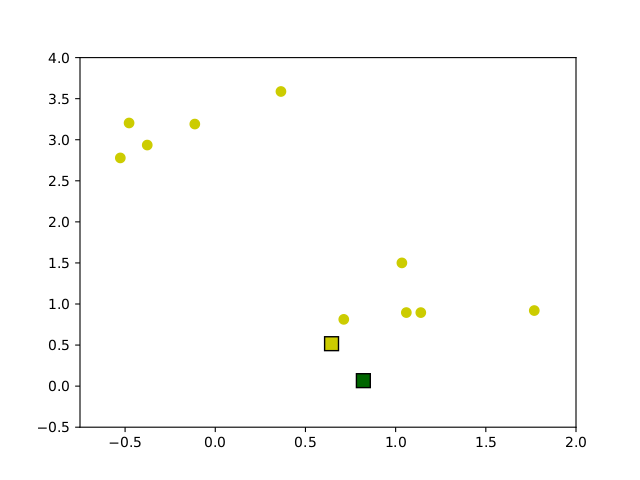
\includegraphics[width=0.4\linewidth]{bilder/06-plot1} 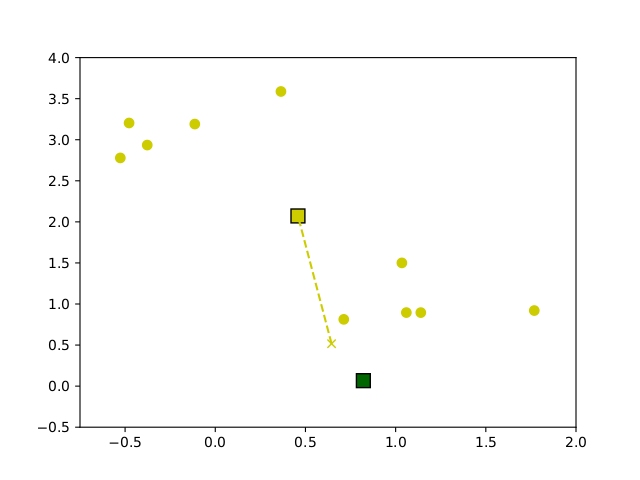
\includegraphics[width=0.4\linewidth]{bilder/06-plot2} 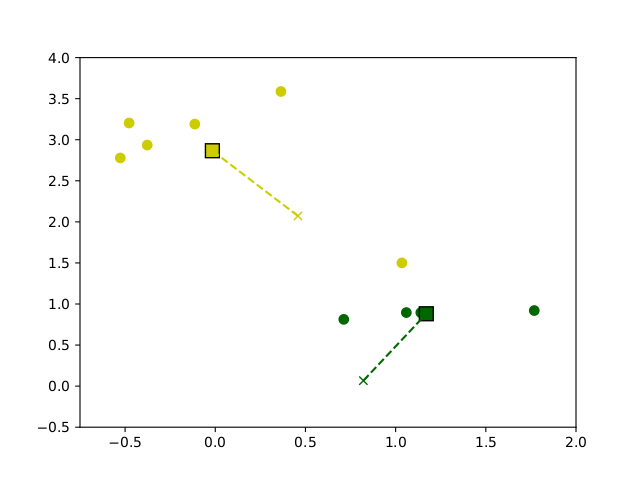
\includegraphics[width=0.4\linewidth]{bilder/06-plot4} 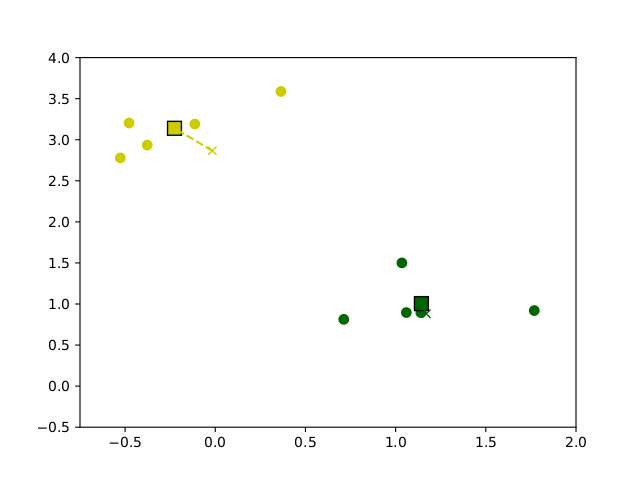
\includegraphics[width=0.4\linewidth]{bilder/06-plot6} 

}

\caption{Entwicklung der Centroids im Verlauf des k-means clustering Algorithmus auf Beispieldaten}\label{fig:k-means-evoexa}
\end{figure}

\hypertarget{clustering-und-hauptkomponentenanalyse-1}{%
\section{Clustering und Hauptkomponentenanalyse}\label{clustering-und-hauptkomponentenanalyse-1}}

Der k-means Algorithmus basiert allein auf der Bestimmung von Abständen und Mittelwerten -- beides kann in beliebigen Dimensionen \(n\) der Daten realisiert werden. Allerdings ist die Klassifizierung in höheren Datendimensionen ungleich schwieriger da

\begin{itemize}
\item
  für eine vergleichsweise ähnlich große Einzugsbereiche, müssen ungleich mehr clusters verwendet werden. Beispielsweise lößt sich ein Quadrat der Seitenlänge 2 in \(4=2^2\) Quadrate der Größe 1 aufteilen. Für einen Würfel (eine Dimension mehr), braucht Jan entsprechend \(8=2^3\) (das heisst doppelt so viele) Unterbereiche. In vier Dimensionen wären es bereits \(2^4\). Und so weiter.
\item
  die Berechnung der Abstände und Zuordnung zu den clusters wird aufwändiger
\item
  es gibt ungleich mehr Konfigurationen für die centroids. Es braucht unter Umständen mehr Iterationen um einen stabilen Zustand zu erreichen.
\end{itemize}

Ein einfacher Zugang wäre es, eine reduzierte Anzahl der Merkmale zur Klassifizierung einzusetzen. Allerdings wird die Qualität der Klassifizierung davon abhöngen, wie geeignet die ausgesuchten Merkmale dafür sind. Ein Blick auf die verschiedenen Plots in Abbildung \ref{fig:05-penguin-allpairs} kann helfen zu verstehen, dass manche Paare von Koordinaten besser als andere geeignet sind um die 3 Pinguinarten zu unterscheiden.

Folgen wir hingegen der Annahme, dass eine hohe Varianz einen hohen Informationsgehalt bedeutet, können wir die Hauptkomponentenanalyse einsetzen um Richtungen von höchster Varianz zu identifizieren und auch Richtungen die überhaupt keine Korrelationen aufzeigen auszuschließen. In der Tat suggerieren die Plots der Pinguindaten in den Hauptkoordinaten (Abbildung \ref{fig:05-penguin-allpairs-pcs}), dass die ersten Hauptrichtungen die Spezies gut unterscheiden, während die letzten Richtungen ein scheinbar zufälliges Rauschen zeigen.

\leavevmode\hypertarget{rem-pca-clustering}{}%
\begin{JHSAYS}
Auch wenn die Hauptrichtungen die Daten nicht unbedingt besser separieren, ermöglichen sie doch das ausschließen der (transformierten) Merkmale ohne Informationsgehalt und damit einen strukturierten und allgemeinen Ansatz zur Klassifizierung hochdimensionaler Daten mit reduzierten Merkmalen.

\end{JHSAYS}

\hypertarget{training-und-testing}{%
\section{Training und Testing}\label{training-und-testing}}

Das Klassifizieren ist ein erstes konkretes Beispiel dafür, wie aus Daten ein Modell abgeleitet wird. Für die gemessenen Pinguine kennen wir die Spezies, das Ziel ist, ein Modell zu haben mit dem wir zukünftig angetroffene Pinguine anhand ihrer gemessenen Merkmale klassifizieren können.

Allgemein wird für einen solchen neuen Datenpunkt wie folgt vorgegangen

\begin{enumerate}
\def\labelenumi{\arabic{enumi}.}
\tightlist
\item
  (Gegebenenfalls) Normalisierung des Datenpunktes durch Skalierung und Abziehen des (zuvor ermittelten) Mittelwertes.
\item
  (Gegebenenfalls) Transformation in (reduzierte) Hauptkoordinaten.
\item
  Test zu welchen centroid \(c_j\), \(j=1,\dots,K\) der (transformierte) Datenpunkt am nächsten liegt.
\end{enumerate}

Der in (3.) ermittelte Index \(j^*\) ist dann das Cluster, dem der Datenpunkt zugeordnet wird.

Der Sprachgebrauch hier ist, dass das Modell mit bekannten Daten \emph{trainiert} wird und dann für neue Daten \emph{angewendet} wird\footnote{Im \emph{machine learning} wird gerne von \emph{generalization} gesprochen}. Um zu evaluieren, ob das Modell ``funktioniert'' ist das folgende Vorgehen ebenso naheliegend wie standardmäßig angewandt.

Die vorhandenen Daten werden aufgeteilt in \textbf{Trainingsdaten}, mit denen das Modell trainiert werden, und \textbf{Testdaten}, mit denen die Vorhersagekraft des Modells evaluiert wird. Wie die Aufteilung passiert, wird anhand von Erfahrungswerten und im Hinblick auf die vorliegende Aufgabe entschieden.

\hypertarget{am-beispiel-der-pinguine}{%
\section{Am Beispiel der Pinguine}\label{am-beispiel-der-pinguine}}

\begin{figure}

{\centering 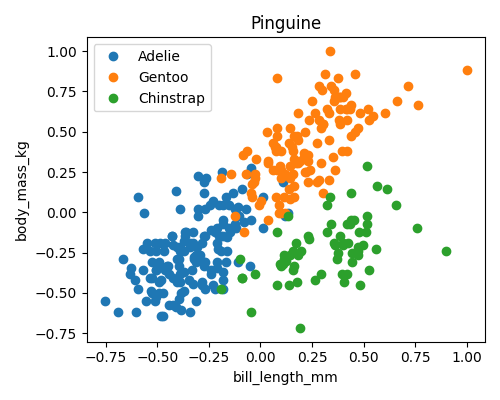
\includegraphics[width=0.8\linewidth]{bilder/06-Figure_10101} 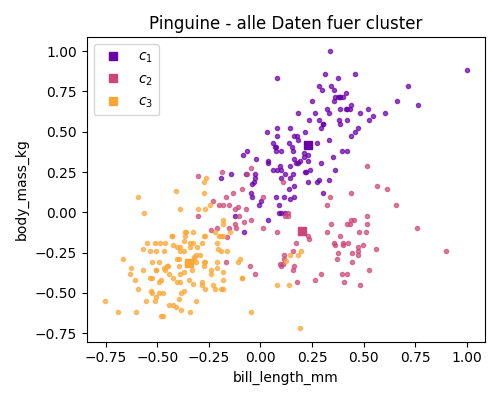
\includegraphics[width=0.8\linewidth]{bilder/06-Figure_101} 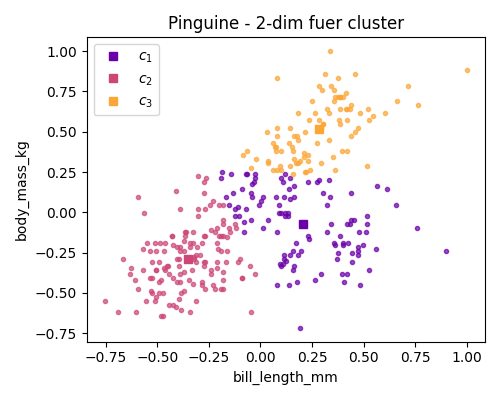
\includegraphics[width=0.8\linewidth]{bilder/06-Figure_111} 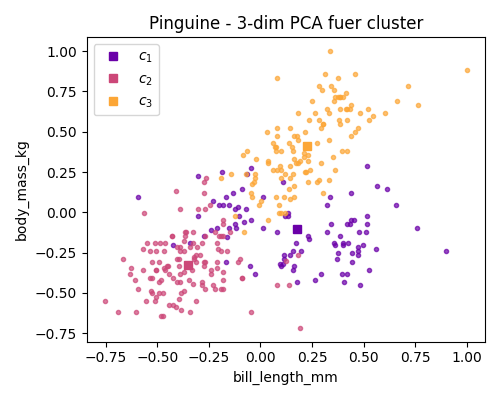
\includegraphics[width=0.8\linewidth]{bilder/06-Figure_121} 

}

\caption{Einige clustering Resultate fuer die Pinguin Daten}\label{fig:k-means-pingexa}
\end{figure}

\begin{figure}

{\centering 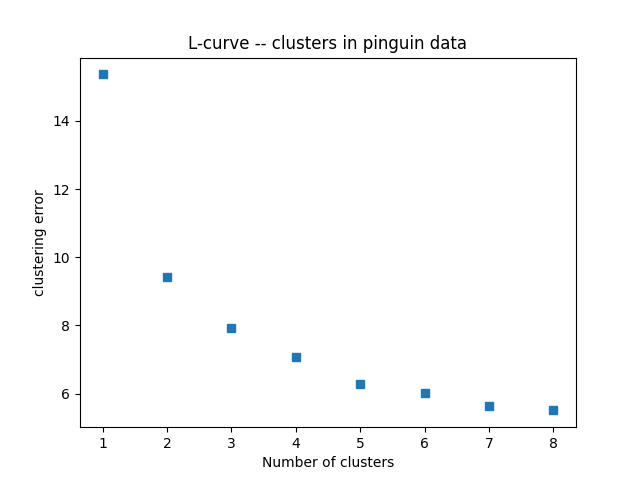
\includegraphics[width=0.8\linewidth]{bilder/06-L-curve} 

}

\caption{Die L-Kurve fuer die Pinguin Daten}\label{fig:k-means-pingexa-lcurve}
\end{figure}

\hypertarget{aufgaben-3}{%
\section{Aufgaben}\label{aufgaben-3}}

\hypertarget{k-means-von-hand-t}{%
\subsection{K-means von Hand (T)}\label{k-means-von-hand-t}}

Führen sie händisch und nach Augenschein zwei Iterationen des K-means Algorithmus auf den vom folgenden Skript erzeugten \texttt{(x,z)} Daten durch. Dazu bitte, Beispielsweise in Abbildung \ref{fig:k-means-evoexaexrcs}, in jedem Schritt die Clusterzugehörigkeiten markieren und die neuen (geschätzten) Mittelpunkte \(c_1\) und \(c_2\) eintragen.

\begin{Shaded}
\begin{Highlighting}[]
\ImportTok{from}\NormalTok{ numpy.random }\ImportTok{import}\NormalTok{ default\_rng}
\ImportTok{import}\NormalTok{ matplotlib.pyplot }\ImportTok{as}\NormalTok{ plt}

\CommentTok{\# Zufallszahlengenerator mit "seed=1"}
\NormalTok{rng }\OperatorTok{=}\NormalTok{ default\_rng(}\DecValTok{1}\NormalTok{)}

\CommentTok{\# Zufallsdaten mit etwas Korrelation fuer z}
\NormalTok{x }\OperatorTok{=}\NormalTok{ rng.beta(}\DecValTok{1}\NormalTok{, }\DecValTok{1}\NormalTok{, }\DecValTok{9}\NormalTok{)}
\NormalTok{y }\OperatorTok{=}\NormalTok{ rng.beta(}\DecValTok{1}\NormalTok{, }\DecValTok{1}\NormalTok{, }\DecValTok{9}\NormalTok{)}
\NormalTok{z }\OperatorTok{=}\NormalTok{ (x}\OperatorTok{*}\NormalTok{x}\OperatorTok{*}\NormalTok{y)}\OperatorTok{**}\NormalTok{(}\DecValTok{1}\OperatorTok{/}\DecValTok{3}\NormalTok{)}

\CommentTok{\# Zufallswahl der initialen centroids}
\NormalTok{cntro }\OperatorTok{=}\NormalTok{ rng.beta(}\DecValTok{1}\NormalTok{, }\DecValTok{1}\NormalTok{, }\DecValTok{2}\NormalTok{)}
\NormalTok{cntrt }\OperatorTok{=}\NormalTok{ rng.beta(}\DecValTok{1}\NormalTok{, }\DecValTok{1}\NormalTok{, }\DecValTok{2}\NormalTok{)}

\NormalTok{plt.figure(}\DecValTok{1}\NormalTok{, figsize}\OperatorTok{=}\NormalTok{(}\DecValTok{5}\NormalTok{, }\DecValTok{3}\NormalTok{))}
\NormalTok{plt.plot(x, z, }\StringTok{\textquotesingle{}.\textquotesingle{}}\NormalTok{, label}\OperatorTok{=}\StringTok{\textquotesingle{}data\textquotesingle{}}\NormalTok{)}
\NormalTok{plt.plot(cntro[}\DecValTok{0}\NormalTok{], cntro[}\DecValTok{1}\NormalTok{], }\StringTok{\textquotesingle{}s\textquotesingle{}}\NormalTok{, label}\OperatorTok{=}\StringTok{\textquotesingle{}$c\_1$\textquotesingle{}}\NormalTok{)}
\NormalTok{plt.plot(cntrt[}\DecValTok{0}\NormalTok{], cntrt[}\DecValTok{1}\NormalTok{], }\StringTok{\textquotesingle{}s\textquotesingle{}}\NormalTok{, label}\OperatorTok{=}\StringTok{\textquotesingle{}$c\_2$\textquotesingle{}}\NormalTok{)}
\NormalTok{plt.legend(loc}\OperatorTok{=}\StringTok{\textquotesingle{}upper left\textquotesingle{}}\NormalTok{)}
\NormalTok{plt.title(}\StringTok{\textquotesingle{}K{-}means: initialer Zustand\textquotesingle{}}\NormalTok{)}
\NormalTok{plt.show()}
\end{Highlighting}
\end{Shaded}

\begin{figure}

{\centering 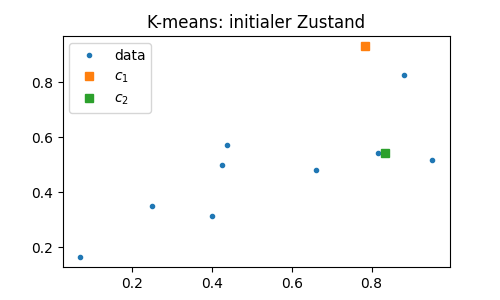
\includegraphics[width=0.8\linewidth]{bilder/06-manual-kmeans-ini} 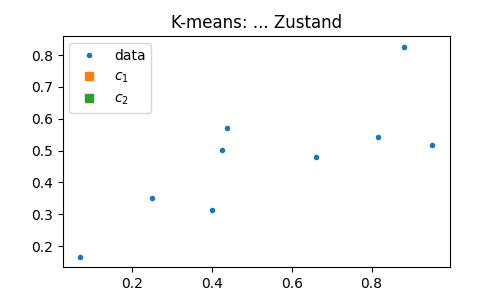
\includegraphics[width=0.8\linewidth]{bilder/06-manual-kmeans-x} 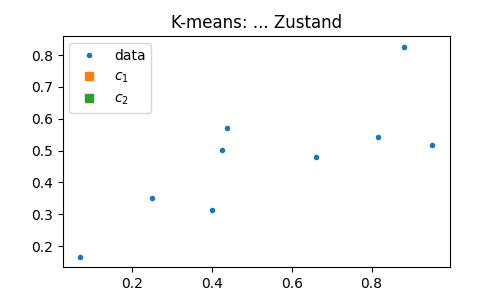
\includegraphics[width=0.8\linewidth]{bilder/06-manual-kmeans-x} 

}

\caption{Bitte gerne hier die Evolution einzeichnen}\label{fig:k-means-evoexaexrcs}
\end{figure}

\hypertarget{k-means-als-algorithmus-p}{%
\subsection{K-means als Algorithmus (P)}\label{k-means-als-algorithmus-p}}

Schreiben sie eine Funktion, die mittels des k-means Algorithmus einen Datensatz in beliebiger Dimension in \texttt{K} vorgegebene cluster gruppiert und die labels der Daten sowie die Koordinaten der centroids zurueckgeben.

Testen sie die Funktion am obigen theoretischen Beispiel.

Hier \href{bilder/kmeans_utils.py}{zum Download angehängt} eine Datei mit ein paar hilfreichen Routinen und schon einer Vorgabe für die ``Hauptroutine''. \textbf{Bitte machen Sie sich damit vertraut, wie in Python Routinen aus einem \emph{module} (d.h. einer anderen Datei mit Python Funktionen) importiert werden kann.}

\begin{Shaded}
\begin{Highlighting}[]
\ImportTok{from}\NormalTok{ kmeans\_utils }\ImportTok{import}\NormalTok{ kmeans, plot\_cluster\_data}
\CommentTok{\# import routines from a module}

\CommentTok{\# construct data as above}
\NormalTok{N }\OperatorTok{=} \DecValTok{9}
\NormalTok{K }\OperatorTok{=} \DecValTok{2}

\NormalTok{x }\OperatorTok{=}\NormalTok{ rng.beta(}\DecValTok{1}\NormalTok{, }\DecValTok{1}\NormalTok{, N)}
\NormalTok{y }\OperatorTok{=}\NormalTok{ rng.beta(}\DecValTok{1}\NormalTok{, }\DecValTok{1}\NormalTok{, N)}
\NormalTok{z }\OperatorTok{=}\NormalTok{ (x}\OperatorTok{*}\NormalTok{x}\OperatorTok{*}\NormalTok{y)}\OperatorTok{**}\NormalTok{(}\DecValTok{1}\OperatorTok{/}\DecValTok{3}\NormalTok{)}

\NormalTok{cntro }\OperatorTok{=}\NormalTok{ rng.beta(}\DecValTok{1}\NormalTok{, }\DecValTok{1}\NormalTok{, }\DecValTok{2}\NormalTok{)}
\NormalTok{cntrt }\OperatorTok{=}\NormalTok{ rng.beta(}\DecValTok{1}\NormalTok{, }\DecValTok{1}\NormalTok{, }\DecValTok{2}\NormalTok{)}

\NormalTok{cntrdlist }\OperatorTok{=}\NormalTok{ [cntro, cntrt]}
\NormalTok{datamatrix }\OperatorTok{=}\NormalTok{ np.hstack([x.reshape((x.size, }\DecValTok{1}\NormalTok{)), z.reshape((z.size, }\DecValTok{1}\NormalTok{))])}

\CommentTok{\# run the kmeans algorithm}
\NormalTok{cntrdlist, labels, cerror }\OperatorTok{=}\NormalTok{ kmeans(datamatrix, K}\OperatorTok{=}\DecValTok{2}\NormalTok{, cntrdlist}\OperatorTok{=}\NormalTok{cntrdlist)}

\CommentTok{\# plot the result}
\NormalTok{plot\_cluster\_data(datamatrix, labels, cntrdlist,}
\NormalTok{                  xlabel}\OperatorTok{=}\StringTok{\textquotesingle{}feature\textquotesingle{}}\NormalTok{, ylabel}\OperatorTok{=}\StringTok{\textquotesingle{}other feature\textquotesingle{}}\NormalTok{,}
\NormalTok{                  fignum}\OperatorTok{=}\DecValTok{10101}\NormalTok{, figsize}\OperatorTok{=}\NormalTok{(}\DecValTok{5}\NormalTok{, }\DecValTok{4}\NormalTok{),}
\NormalTok{                  titlestr}\OperatorTok{=}\StringTok{\textquotesingle{}K{-}means: finaler Zustand\textquotesingle{}}\NormalTok{)}
\end{Highlighting}
\end{Shaded}

\hypertarget{k-means-fuer-die-pinguine}{%
\subsection{K-means fuer die Pinguine}\label{k-means-fuer-die-pinguine}}

Wenden sie den Algorithmus auf die (zentrierten und auf in jeder Richtung auf \([-1, 1]\) skalierten) Pinguindaten an. Und vergleichen sie mit den Bildern oben.

\begin{enumerate}
\def\labelenumi{\arabic{enumi}.}
\tightlist
\item
  In der gesamten Datendimension
\item
  Für zwei beliebig gewählte Merkmale
\item
  Für die ersten drei Hauptkomponenten
\end{enumerate}

\begin{Shaded}
\begin{Highlighting}[]
\ImportTok{import}\NormalTok{ json}

\ImportTok{import}\NormalTok{ numpy }\ImportTok{as}\NormalTok{ np}
\ImportTok{import}\NormalTok{ matplotlib.pyplot }\ImportTok{as}\NormalTok{ plt}

\ImportTok{from}\NormalTok{ kmeans\_utils }\ImportTok{import}\NormalTok{ kmeans}

\ControlFlowTok{with} \BuiltInTok{open}\NormalTok{(}\StringTok{\textquotesingle{}penguin{-}data.json\textquotesingle{}}\NormalTok{, }\StringTok{\textquotesingle{}r\textquotesingle{}}\NormalTok{) }\ImportTok{as}\NormalTok{ f:}
\NormalTok{    datadict }\OperatorTok{=}\NormalTok{ json.load(f)}

\NormalTok{data }\OperatorTok{=}\NormalTok{ np.array(datadict[}\StringTok{\textquotesingle{}data\textquotesingle{}}\NormalTok{])}

\CommentTok{\# center and scale}
\NormalTok{data }\OperatorTok{=}\NormalTok{ data }\OperatorTok{{-}}\NormalTok{ data.mean(axis}\OperatorTok{=}\DecValTok{0}\NormalTok{)}
\NormalTok{maxvals }\OperatorTok{=}\NormalTok{ np.}\BuiltInTok{max}\NormalTok{(np.}\BuiltInTok{abs}\NormalTok{(data), axis}\OperatorTok{=}\DecValTok{0}\NormalTok{)}
\NormalTok{data }\OperatorTok{=}\NormalTok{ data }\OperatorTok{*} \DecValTok{1}\OperatorTok{/}\NormalTok{maxvals}
\CommentTok{\# now the data has zero mean and is scaled to fit into [{-}1, 1]}
\end{Highlighting}
\end{Shaded}

\leavevmode\hypertarget{clustering-random}{}%
\begin{JHSAYS}
Achtung -- auch hier ist wieder Zufall involviert. Wenn das Ergebnis seltsam aussieht, gegebenfalls das Experiment mehrfach wiederholen um auszuschließen, dass es sich nur um einen statistischen Ausreißer handelt.

\end{JHSAYS}

\hypertarget{l-curve}{%
\subsection{L-curve}\label{l-curve}}

Bestimmen sie die L-Kurve fuer die Pinguindaten fuer \texttt{K=1,2,3,4,...,8} -- fuer das clustering auf dem gesamten Datensatz.

\hypertarget{optimierung}{%
\chapter{Optimierung}\label{optimierung}}

\providecommand{\diva}[1]{\mathrm{d} #1}

Einige Optimierungsprobleme haben wir schon kennengelernt und zwar

\begin{itemize}
\tightlist
\item
  bei der linearen Regression (vgl. besonders Kapitel \ref{sec-linreg-minimierung}) bei der die Parameter der Ansatzfunktion \textbf{bestmöglich} an die Daten gefittet wurden
\item
  bei der Hauptkomponentenanalyse (vgl. besonders Kapitel \ref{sec-pca-maximierung}) als wir die Hauptrichtungen so ermittelt, dass in ihrer Richtung die Varianz \textbf{maximal} wurde.
\end{itemize}

Hier lag in beiden Fällen ein sogenanntes linear-quadratisches Optimierungsproblem vor, für welche die Existenz der Lösungen bewiesen werden kann und die mit Methoden aus der linearen Algebra direkt gelöst werden können.

Sogenannte \emph{nichtlineare Optimierungsprobleme} liegen vor, wenn die zu erfüllenden Ziele wirklich nichtlineare Gleichungen enthalten. Zum Bespiel sind gängige Elemente von \emph{Neuronalen Netzen} als
\begin{equation*}
f(x) = \tanh(a\, x + b)
\end{equation*}
gegeben, mit Parametern \(a\), \(b\) die aus der Minimierung eines \emph{mean square error} Terms der Form
\begin{equation*}
\frac 1N \sum_{k=1}^N|y_k - \tanh(a\, x_k + b)|^2
\end{equation*}
für gegebene Trainingsdaten \((x_k, y_k)\) bestimmt werden.

Wir sehen, dass die Optimierung ein ganz wesentlicher Teil der \emph{Data Science} ist (und ganz unabhängig davon ein eigenes Forschungsgebiet ist und quasi überall in der Praxis mittel-- oder unmittelbar benutzt wird).

Nachfolgend ein paar Begriffe aus der Optimierung

\begin{itemize}
\tightlist
\item
  \emph{glatte Optimierung} -- das Modell beinhaltet ausreichend stetige (bzw. differenzierbare) Funktionen. Ein Optimum könnte durch Bestimmung von Ableitungen berechnet werden.
\item
  \emph{nichtglatte Optimierung} -- das Modell beinhaltet Teile, die nicht differenzierbar sind. Das kann am Problem selbst liegen oder, was bei \emph{machine learning} im Speziellen und \emph{Data Science} an sich eine Rolle spielt, dass die Daten verrauscht sind. Jetzt ist eine (klassische) Ableitung nicht mehr möglich aber es existieren diverse Ansätze zur Abhilfe.
\item
  \emph{diskrete Optimierung} -- in obigen Fällen sind wir implizit davon ausgegangen, dass die Lösung und die Gleichungen auf den reellen oder komplexen Zahlen leben. Denkbar ist aber auch, dass diskrete Lösungen (z.B. Anzahlen oder binäre Zustände) gesucht werden.
\item
  \emph{kombinatorische Optimierung} -- hier ergeben sich die möglichen Lösungen als Kombination von Möglichkeiten. Oft ist die Anzahl möglicher Lösungen endlich aber sehr groß.
\item
  \emph{restringierte Optimierung} -- zusätzlich zu einem Optimalitätskriterium sind noch Nebenbedingungen zu erfüllen.
\end{itemize}

Hier werden wir uns erstmal mit glatter Optimierung ohne Nebenbedingungen beschäftigen.

\hypertarget{multivariable-funktionen}{%
\section{Multivariable Funktionen}\label{multivariable-funktionen}}

Um unsere Optimierungsprobleme in allgemeiner Form zu formulieren und auch um allgemeine Lösungsansätze herzuleiten, brauchen wir erstmal ein paar Begriffe aus der Analysis von multivariablen Funktionen.

Es sei also eine Funktion
\begin{equation*}
f\colon \mathbb R^{n}\to \mathbb R^{}, \quad f \colon (x_1,x_2, \dots, x_n) \mapsto f(x_1, x_2, \dotsc, x_n)
\end{equation*}
gegeben, die ein \(n\)-tupel von Variablen auf einen reellen Wert abbildet. Ein Beispiel wäre
\begin{equation*}
g(x_1, x_2, x_3) = \sin(x_1) + x_3\cos(x_2) + x_1^2 x_2^2 x_3^2 - 2x_2.
\end{equation*}

\leavevmode\hypertarget{variablen-namen}{}%
\begin{JHSAYS}
Hier verwenden wir jetzt \(x_i\) für die \(i\)-te Variable der multivariablen Funktion. Bitte nicht verwechseln mit der Bezeichnung für den \(i\)-ten Datenpunkt zum Beispiel in Kapitel \ref{sec-lineare-regression}.

Außerdem wäre es besser wir würden die Funktion mit einem Definitionsbereich \(D(f)\) angeben, also schreiben
\begin{equation*}
f\colon D(f) \subset \mathbb R^{n}\to \mathbb R^{}
\end{equation*}
da eine Funktion eventuell nicht überall definiert ist (bzw. definiert sein muss). Im Sinne der besseren Lesbarkeit, ersparen wir uns dieses Detail.

\end{JHSAYS}

\hypertarget{partielle-ableitungen-und-der-gradient}{%
\section{Partielle Ableitungen und der Gradient}\label{partielle-ableitungen-und-der-gradient}}

Wenn wir alle Variablen bis auf die \(i\)-te für einen Augenblick einfrieren (also auf einen konstanten Wert \(\bar x_j\) festlegen und nicht verändern), können wir die Teilfunktion
\begin{equation*}
\bar f_{(i)}\colon \mathbb R^{}\to \mathbb R^{}, \quad \bar f_{(i)}\colon x_i \to f(\bar x_1, \dotsc, \bar x_{i-1}, x_i, \bar x_{i+1}, \dotsc, \bar x_n)
\end{equation*}
als Funktion mit einer Veränderlichen (und \(n-1\) Parametern) betrachten und wie gehabt ableiten. Die erhaltene, sogenannte \emph{partielle Ableitung} hängt von den Parametern \(\bar x_j\) ab und wird mit
\begin{equation*}
\frac{\partial f}{\partial x_i}
\end{equation*}
bezeichnet. Alle \(n\) möglichen partiellen Ableitungen in einen Vektor geschrieben ergeben den sogenannten \emph{Gradienten}
\begin{equation*}
\nabla f = 
\begin{bmatrix}
\frac{\partial f}{\partial x_1} \\
\frac{\partial f}{\partial x_2} \\
\vdots \\
\frac{\partial f}{\partial x_n}
\end{bmatrix}
\colon \mathbb R^{n} \to \mathbb R^{n},
\end{equation*}
der wiederum eine (vektorwertige) Funktion von \(n\) Variablen ist.
Für unser obiges Beispiel bekommen wir
\begin{equation*}
\nabla g(x_1, x_2, x_3) =
\begin{bmatrix}
\cos(x_1)+2x_1x_2^2x_3^2\\
-x_3\sin(x_2) + x_1^2x_2x_3^2 - 2 \\
\cos(x_2) + 2x_1^2x_2^2x_3
\end{bmatrix}
\end{equation*}

\hypertarget{richtungs-ableitung}{%
\section{Richtungs-Ableitung}\label{richtungs-ableitung}}

Die Betrachtung der Funktionen \(\bar f_{(i)}\) ermöglicht die Analysis des Verhaltens der Funktion entlang der \(i\)-ten Koordinaten Richtung. Um die Funktion in einer beliebigen Richtung um einen festen Punkt
\begin{equation*}
\bar x = (\bar x_1, \bar x_2, \dotsc, \bar x_n)
\end{equation*}
zu untersuchen, kann die Funktion entlang einer Richtung \(v \in \mathbb R^{n}\) parametrisiert werden:
\begin{equation*}
\bar f_{(v)} \colon \mathbb R^{} \to \mathbb R^{}, \quad t \mapsto \bar f_{(v)}(t) = f(\bar x + tv)
\end{equation*}

\leavevmode\hypertarget{richtung-is-partiell}{}%
\begin{JHSAYS}
Für \(v=e_i\) bekommen wir direkt, dass \(\bar f_{(v)}=\bar f_{(i)}\).

\end{JHSAYS}

Wiederum handelt es sich um eine reelle Funktion in einer Variablen (hier der Parameter \(t\)), die wir schulbuchmäßig ableiten könnten. Für diese sogenannte \emph{Richtungsableitung} gilt der folgende Zusammenhang\footnote{Das folgt aus der Kettenregel für multivariable Funktionen, die wir in der Vorlesung \emph{Mathematik für Data Science 2} noch beweisen werden}
\begin{equation*}
\frac{\mathrm{d} \bar f_{(v)}}{\mathrm{d} t}(0) = \sum_i^n \frac{\partial f}{\partial x_i}(\bar x_i) v_i = \langle \nabla f(\bar x), v \rangle
\end{equation*}

\leavevmode\hypertarget{richtung-ableitung}{}%
\begin{JHSAYS}
Die Veränderungsrate der Funktion \(f\) im Punkt \(\bar x\) in der Richtung von \(v\) ist gleich dem Skalarprodukt aus Gradient im Punkt \(\bar x\) und der gewählten Richtung.

\end{JHSAYS}

Sei nun \(v\) normiert, also \(\|v\|=1\), dann gilt nach der Winkelformel, dass
\begin{equation*}
\langle \nabla f(\bar x), v \rangle = \|\nabla f(\bar x) \| \cos (\alpha)
\end{equation*}
wobei \(\alpha\) der von \(\nabla f(\bar x)\) und \(v\) eingeschlossene Winkel ist. Wir bemerken, dass die Veränderung maximal wird, wenn \(\alpha = 0\) oder
\begin{equation*}
v = \frac{1}{ \| \nabla f(\bar x) \| } \nabla f(\bar x)
\end{equation*}
als ein Vielfaches des Gradientenvektors gewählt wird.
Andersherum können wir einige ganz wesentliche Aspekte folgern:

\begin{itemize}
\tightlist
\item
  der Gradient selbst in die Richtung des stärksten Anstiegs
\item
  der negative Gradient \(-\nabla f(\bar x)\) zeigt in die Richtung des stärksten Abfalls
\item
  ist der Gradient der Nullvektor, dann findet keine Veränderung mehr statt, d.h. dass aus \(\nabla f(\bar x) =0\) folgt, dass \(\bar x\) ein kritischer Punkt von \(f\) ist
\item
  ist der Gradient nicht der Nullvektor, kann \(\bar x\) kein Minimum und kein Maximum sein (weil die Funktion in \(-\nabla f(\bar x)\) Richtung abfällt und in \(\nabla f(\bar x)\) Richtung ansteigt)
\end{itemize}

\hypertarget{optimierung-1}{%
\section{Optimierung}\label{optimierung-1}}

Ganz allgemein können wir unsere bisherigen Optimierungsprobleme schreiben als
\begin{equation*}
f(x) \to \min_{x\in \mathbb R^{n}},
\end{equation*}
das heißt für eine Funktion \(f\colon \mathbb R^n \to \mathbb R^{}\) suchen wir das \(x \in D(f) \subset \mathbb R^{n}\), für das \(f(x)\) minimal wird.

\begin{definition}
\protect\hypertarget{def:loc-glob-minimum}{}\label{def:loc-glob-minimum}

Gegeben sei \(f\colon \mathbb R^{n} \to \mathbb R^{}\). Wir nennen \(x^* \in D(f)\subset \mathbb R^{n}\) die Stelle

\begin{itemize}
\item
  eines \emph{lokales Minimum} (von \(f\)) falls es ein \(\epsilon >0\) gibt, sodass
  \begin{equation*}
  f(x^*) \leq f(x)
  \end{equation*}
  für alle \(x \in D(f) \cap B_\epsilon (x^*)\).
\item
  eines globales Minimum, falls \(f(x^*) \leq f(x)\) für alle \(x\in D(f)\) ist.
\end{itemize}

\end{definition}

In dieser Definition benutzen wir ``\(\leq\)'', da das im Hinblick auf Minimierung (der Wert von \(f\) ist wichtig, die Stelle, an der das Minimum angenommen wird, ist weniger entscheidend) praktikabel ist. Wir könnten aber auch von strikten (oder ``echten'') Minima sprechen und ``\(<\)'' verlangen.

Der Schnitt der Umgebung
\[ B_\epsilon(x^*) := \{x\in \mathbb R^{n}| \|x-x^*\|< \epsilon\} \]
mit dem Definitionsbereich \(D(f)\) ist relevant, wenn \(x^*\) genau auf dem Rand des Definitionsbereichs liegt.

Nun erstmal ein hinreichendes Kriterium für ein Extremum
(vgl. Thm. 2.2, Nocedal and Wright \protect\hyperlink{ref-NocW06}{2006}):

\begin{theorem}
Sei \(D(f) \subseteq \mathbb{R}^{n}\) offen, und sei \(f\colon D(f) \rightarrow \mathbb{R}\) stetig partiell differenzierbar. Besitzt \(f\) in \(\mathbf{x}^{*} \in D(f)\) ein lokales Extremum\footnote{könnte auch ein Maximum sein, was wir aber einfach als ein Minimum von \(-f\) einordnen}, dann ist \(\nabla f(\mathbf{x}^{*})=0\).
\end{theorem}

\begin{JHSAYS}
Das können wir wie in der einfachen Kurvendiskussion verstehen: \emph{Liegt in \(x^*\) ein Extremum vor und \(x^*\) liegt nicht auf dem Rand, so verschwindet die erste Ableitung.} Um festzustellen, ob ein Minimum, Maximum und vor allem nicht einfach ein Sattelpunkt vorliegt, wurde geschaut ob die zweite Ableitung positiv, negativ oder gleich 0 ist. Bei multivariablen Funktionen wird die zweite Ableitung durch eine Matrix repräsentiert. Und positiv, negativ oder indefinit wird wird über die Eigenwerte definiert.

\end{JHSAYS}

\begin{definition}[Hesse-Matrix]
Sei \(D(f) \subseteq \mathbb{R}^{n}\) offen, und sei \(f\colon D(f) \rightarrow \mathbb{R}\) eine 2-mal stetig partiell differenzierbare Funktion. Für \(\mathbf{x}^{\star} \in D\) heißt die symmetrische \((n \times n)\)-Matrix
\[
H_{f}\left(\mathbf{x}^{\star}\right)=\left(\begin{array}{cccc}
\frac{\partial^{2} f}{\partial x_{1} \partial x_{1}}\left(\mathbf{x}^{\star}\right) & \frac{\partial^{2} f}{\partial x_{2} \partial x_{1}}\left(\mathbf{x}^{\star}\right) & \cdots & \frac{\partial^{2} f}{\partial x_{n} \partial x_{1}}\left(\mathbf{x}^{\star}\right) \\
\frac{\partial^{2} f}{\partial x_{1} \partial x_{2}}\left(\mathbf{x}^{\star}\right) & \frac{\partial^{2} f}{\partial x_{2} \partial x_{2}}\left(\mathbf{x}^{\star}\right) & \cdots & \frac{\partial^{2} f}{\partial x_{n} \partial x_{2}}\left(\mathbf{x}^{\star}\right) \\
\vdots & \vdots & \cdots & \vdots \\
\frac{\partial^{2} f}{\partial x_{1} \partial x_{n}}\left(\mathbf{x}^{\star}\right) & \frac{\partial^{2} f}{\partial x_{2} \partial x_{n}}\left(\mathbf{x}^{\star}\right) & \cdots & \frac{\partial^{2} f}{\partial x_{n} \partial x_{n}}\left(\mathbf{x}^{\star}\right)
\end{array}\right)
\]
Hesse-Matrix von \(f\) in \(\mathbf{x}^{\star}\).
\end{definition}

Hierbei ist \(\frac{\partial^{2} f}{\partial x_{i} \partial x_{j}}:=\frac{\partial }{\partial x_{i}}(\frac{\partial f}{\partial x_{j}})\) die wiederholte partielle Differentiation in möglicherweise verschiedene Koordinatenrichtungen. Die postulierte Symmetrie der Hesse-Matrix folgt aus der Gleichheit
\begin{equation*}
\frac{\partial }{\partial x_{i}}(\frac{\partial f}{\partial x_{j}})
=
\frac{\partial }{\partial x_{j}}(\frac{\partial f}{\partial x_{i}})
\end{equation*}
deren Gültigkeit wir noch in der Mathematik Vorlesung beweisen werden. Als nächstes ein Hinreichendes Kriterium für Minimalität (vgl. Theorem 2.4, Nocedal and Wright \protect\hyperlink{ref-NocW06}{2006}):

\begin{theorem}[Hinreichende Optimalitätsbedingung zweiter Ordnung]
Sei \(D(f) \subset \mathbb{R}^{n}\) offen, und sei \(f\colon D(f) \rightarrow \mathbb{R}\) eine 2-mal stetig partiell differenzierbare Funktion. Sei \(x^{\star} \in D(f)\) mit \(\nabla f ({x}^{\star})={0}\)
Ist \(H_{f}({x}^{\star})\) positiv definit, dann ist \(\mathbf{x}^{\star}\) ein lokales Minimum.
\end{theorem}

Ein paar Bemerkungen dazu

\begin{itemize}
\item
  Eine symmetrische Matrix \(M\) heißt \emph{positiv definit}, wenn \(x^TMx>0\) ist für alle \(x\in \mathbb R^{n}\setminus \{0\}\). Wir schreiben \(M \prec 0\).
\item
  Hinreichende Kriterien dafür sind

  \begin{itemize}
  \tightlist
  \item
    alle Eigenwerte sind positiv oder
  \item
    alle Hauptminoren sind positiv (das sind die Determinante der Matrizen, die aus \(M\) durch Streichung der letzten \(r\) Zeilen und Spalten entstehen \(r=0,1,\dotsc, n-1\).)
  \end{itemize}
\item
  Ist \(-M \prec 0\), dann liegt ein lokales Minimum von \(-f\) vor (oder eben ein Maximum von \(f\))
\item
  Gilt \(M \preccurlyeq 0\) (also \(M\) ist positiv semidefinit, das heißt die Eigenwerte sind nur ``\(\geq 0\)'' bzw. es gilt nur \(x^TMx\geq 0\)), dann ist \textbf{keine} Aussage möglich.
\item
  Ist die Matrix bestimmt indefinit, also alle Eigenwerte ``\(\neq 0\)'' aber manche positiv und manche negativ, dann liegt ein Sattelpunkt vor (und sicher kein Extremum).
\end{itemize}

\hypertarget{gradientenabstiegsverfahren}{%
\section{Gradientenabstiegsverfahren}\label{gradientenabstiegsverfahren}}

Aus dem Wissen, dass in einem Minimum \(x^*\), der Gradient \(\nabla f(x^*)\) verschwindet und dass in einem beliebigen Punkt \(x^0\) (der kein Extremum ist), der negative Gradient \(-\nabla f(x^0)\) in die Richtung des stärksten Abstiegs zeigt, ergibt sich der folgende Zusammenhang:

\begin{quote}
Für einen beliebigen Startpunkt \(x^0\) gibt es eine Schrittweite \(\alpha^0\), so dass
\[f(x^1) := f(x^0 - \alpha^0 \nabla f(x^0)) < f(x_0) \]
\end{quote}

Das heißt in einem Startpunkt können wir einen kleinen Schritt in die Richtung des stärksten Abstiegs gehen und so die Funktion etwas minimieren. Das wiederholte Anwenden dieses Prinzips ergibt das Gradientenabstiegsverfahren,
\[f(x^{n+1}) := f(x^n - \alpha^n \nabla f(x^n)) < f(x_n) \],
das die Funktion immer weiter minimiert bis entweder der Definitionsbereich verlassen ist oder ein kritischer Punkt mit \(\nabla f(x^k)=0\) erreicht wurde. An diesem könnte nun die Hessematrix ausgewertet werden um festzustellen ob tatsächlich ein Minimum vorliegt.

\begin{itemize}
\item
  Neben der Berechnung des Gradienten, die für große Dimensionen sehr aufwändig werden kann, ist die Bestimmung der Schrittweite \(\alpha^k\) in jedem Schritt entscheidend.

  \begin{itemize}
  \tightlist
  \item
    Dazu kann beispielsweise in jeder Iteration die skalare Funktion \(\alpha \mapsto f(x^{k} - \alpha \nabla f(x^k))\) minimiert werden (\emph{exact line search})
  \item
    Da das aber auch aufwändig sein kann, wurden zahlreiche Approximationen an diese Zwischenoptimierung entwickelt (\emph{inexact line search}).
  \item
    Vgl. auch den Wikipedia Artikel zum \href{https://de.wikipedia.org/wiki/Gradientenverfahren\#Bestimmen_der_Schrittweite}{Gradientenverfahren\#Bestimmen\_der\_Schrittweite}
  \end{itemize}
\item
  Für passend gewählte Schrittweiten und wenn \(f\) hinreichend glatt ist (der Gradient soll Lipshitz-stetig sein), lässt sich Konvergenz und sogar Konvergenzrate der Iteration zu einem stationären Punkt \(x^*\) mit \(\nabla f(x^*)=0\) bestimmen (vgl. Section 3.2 in Nocedal and Wright \protect\hyperlink{ref-NocW06}{2006}).
\item
  Um tatsächlich die Konvergenz zu einem Minimum zu beweisen, wird beispielsweise vorausgesetzt, dass ein striktes lokales Minimum existiert (\emph{lokale Konvexität}) und dass die Hesse-Matrix stetig ist (also \(f\) zweimal stetig partiell differenzierbar ist) (vgl. Section 3.2 in Nocedal and Wright \protect\hyperlink{ref-NocW06}{2006}).
\item
  Wir können uns leicht überlegen, dass dieser Algorithmus immer zu einem lokalen Minimum konvergieren wird und das entscheidend von der Wahl des Startpunktes abhängt.
\end{itemize}

\hypertarget{extra-nichtglatte-optimierung}{%
\section{Extra: Nichtglatte Optimierung}\label{extra-nichtglatte-optimierung}}

Ist die Zielfunktion nicht differenzierbar (oder ist die Berechnung des Gradienten zu aufwändig) kann auf Optimierungsverfahren zurückgegriffen werden, die keinen Gradienten benötigen. Die bekanntesten sind

\begin{itemize}
\tightlist
\item
  \emph{Nelder-Mead} oder auch (\emph{nonlinear Simplex}) Verfahren: Berechnet für \(n+1\) Stützpunkte (ein Simplex im \(\mathbb R^{n}\) die Werte von \(f\) und ersetzt den \emph{schlechtesten} nach Kriterien die eine (vergleichsweise) schnelle Konvergenz zu einem lokalen Minimum garantieren können.
\item
  Sogenannte \emph{generische} oder \emph{genetische Algorithmen}: nach dem Prinzip der Variation (oder Mutation) und Selektion wird der Suchraum \(D(f)\) in zufälliger Weise aber mit einer gewissen Systematik abgesucht -- diese Algorithmen konvergieren (in Wahrscheinlichkeit) zu einem globalen Minimum sind aber vergleichsweise langsam bzw. rechenaufwändig.
\end{itemize}

\hypertarget{extra-automatisches-differenzieren}{%
\section{Extra: Automatisches Differenzieren}\label{extra-automatisches-differenzieren}}

Wir sehen, dass in der glatten Optimierung die Berechnung des Gradienten die wichtigste und gleichzeitig aufwändigste Komponente ist. Kann der Gradient analytisch berechnet und als Funktion zur Verfügung gestellt werden, ist dieses Problem elegant umgangen. In der Praxis sind die Probleme aber oft als eine mehrschichitige Verknüpfung von Funktionen in einem Programmcode gegeben. Andererseits sind die kleinste Elemente dieser Funktion typischerweise Elementarfunktionen, die einfach und analytisch differenziert werden können.

Die Darstellung einer Funktion, zum Beispiel,
\begin{equation*}
f(x_1, x_2) = \|(x_1, x_2)\| = \sqrt{x_1^2 + x_2^2}
\end{equation*}
die als Koordinatenfunktion für \(x_1\) dargestellt werden kann als
\[
\tilde f_1(x_1, z) = g_3(g_2(g_1(x_1); z)), \quad g_3(y) = \sqrt y, \quad g_2(y;z) = y + z^2, \quad g_1(y) = y^2
\]
und mittels Kettenregel die partielle Ableitung als Kombination elementarer Ableitungen berechnet als
\begin{equation*}
\frac{\partial f}{\partial x_1}(x_1,x_2) = g_3'(g_2(g_1(x_1); x_2))\cdot g_2'(g_1(x_1); x_2)\cdot g_1'(x_1)
\end{equation*}

macht sich \emph{Automatisches Differenzieren} zu Nutze und kann zu einem Programmcode

\begin{Shaded}
\begin{Highlighting}[]
\KeywordTok{def}\NormalTok{ ffun(x):}
    \CommentTok{\# ..... alles was f machen soll}
    \ControlFlowTok{return}\NormalTok{ fx}
\end{Highlighting}
\end{Shaded}

einen Programmcode erzeugen, der \texttt{grad\_ffun(x)} berechnet. Das ist der sogenannten Vorwärtsmodus des \emph{Automatischen Differenzierens}.

Der sogenannte \emph{Rückwärtsmodus} ist effizienter und kann leicht ein Programme eingebaut werden und damit zu jeder Funktionsevalution, direkt den Gradienten an dieser Stelle mitliefern.

\begin{JHSAYS}
Die systematische Verwendung des \emph{Automatischen Differenzierens} ist einer der wesentlichsten Garanten für den Erfolg von \emph{machine learning}, da AD das träinieren von grossen Netzwerken überhaupt erst möglich macht.

\end{JHSAYS}

\hypertarget{aufgaben-4}{%
\section{Aufgaben}\label{aufgaben-4}}

\hypertarget{numerische-berechnung-des-gradienten-pt}{%
\subsection{Numerische Berechnung des Gradienten (P+T)}\label{numerische-berechnung-des-gradienten-pt}}

Berechnen sie näherungsweise den Gradienten der Beispielfunktion
\begin{equation*}
f(x_1, x_2, x_3) = \sin(x_1) + x_3\cos(x_2) + - 2x_2 + x_1^2 + x_2^2 + x_3^2
\end{equation*}
(\textbf{Achtung} dieses \(f\) ist nur fast das \(g\) wie oben)
im Punkt \((x_1, x_2, x_3) = (1, 1, 1)\),
indem sie die partiellen Ableitungen durch den Differenzenquotienten, z.B.,
\begin{equation*}
\frac{\partial g}{\partial x_2}(1, 1, 1) \approx \frac{g(1, 1+h, 1) - g(1, 1,1)}{h}
\end{equation*}
für \(h\in\{10^{-3}, 10^{-6}, 10^{-9}, 10^{-12}\}\) berechnen. Berechnen sie auch die Norm der Differenz zum exakten Wert von \(\nabla g(1, 1, 1)\) (s.o.) und interpretieren sie die Ergebnisse.

\begin{Shaded}
\begin{Highlighting}[]
\ImportTok{import}\NormalTok{ numpy }\ImportTok{as}\NormalTok{ np}
 
\KeywordTok{def}\NormalTok{ gfun(x):}
    \ControlFlowTok{return}\NormalTok{ np.sin(x[}\DecValTok{0}\NormalTok{]) }\OperatorTok{+}\NormalTok{ x[}\DecValTok{2}\NormalTok{]}\OperatorTok{*}\NormalTok{np.cos(x[}\DecValTok{1}\NormalTok{]) }\OperatorTok{\textbackslash{}}
        \OperatorTok{{-}} \DecValTok{2}\OperatorTok{*}\NormalTok{x[}\DecValTok{1}\NormalTok{] }\OperatorTok{+}\NormalTok{ x[}\DecValTok{0}\NormalTok{]}\OperatorTok{**}\DecValTok{2} \OperatorTok{+}\NormalTok{ x[}\DecValTok{1}\NormalTok{]}\OperatorTok{**}\DecValTok{2} \OperatorTok{\textbackslash{}}
        \OperatorTok{+}\NormalTok{ x[}\DecValTok{2}\NormalTok{]}\OperatorTok{**}\DecValTok{2}

\KeywordTok{def}\NormalTok{ gradg(x):}
    \ControlFlowTok{return}\NormalTok{ np.array([np.NaN,}
                     \OperatorTok{{-}}\NormalTok{x[}\DecValTok{2}\NormalTok{]}\OperatorTok{*}\NormalTok{np.sin(x[}\DecValTok{1}\NormalTok{]) }\OperatorTok{{-}} \DecValTok{2} \OperatorTok{+} \DecValTok{2}\OperatorTok{*}\NormalTok{x[}\DecValTok{1}\NormalTok{],}
\NormalTok{                     np.NaN]).reshape((}\DecValTok{3}\NormalTok{, }\DecValTok{1}\NormalTok{))}


\CommentTok{\# Inkrement}
\NormalTok{h }\OperatorTok{=} \FloatTok{1e{-}3}

\CommentTok{\# der x{-}wert und das h{-}Inkrement in der zweiten Komponente}
\NormalTok{xzero }\OperatorTok{=}\NormalTok{ np.ones((}\DecValTok{3}\NormalTok{, }\DecValTok{1}\NormalTok{))}
\NormalTok{xzeroh }\OperatorTok{=}\NormalTok{ xzero }\OperatorTok{+}\NormalTok{ np.array([}\DecValTok{0}\NormalTok{, h, }\DecValTok{0}\NormalTok{]).reshape((}\DecValTok{3}\NormalTok{, }\DecValTok{1}\NormalTok{))}

\CommentTok{\# partieller Differenzenquotient}
\NormalTok{dgdxtwo }\OperatorTok{=} \DecValTok{1}\OperatorTok{/}\NormalTok{h}\OperatorTok{*}\NormalTok{(gfun(xzeroh) }\OperatorTok{{-}}\NormalTok{ gfun(xzero))}
\CommentTok{\# Alle partiellen Ableitungen ergeben den Gradienten}
\NormalTok{hgrad }\OperatorTok{=}\NormalTok{ np.array([np.NaN, dgdxtwo, np.NaN]).reshape((}\DecValTok{3}\NormalTok{, }\DecValTok{1}\NormalTok{))}

\CommentTok{\# Analytisch bestimmter Gradient}
\NormalTok{gradx }\OperatorTok{=}\NormalTok{ gradg(xzero)}

\CommentTok{\# Die Differenz in der Norm}
\NormalTok{hdiff }\OperatorTok{=}\NormalTok{ np.linalg.norm((hgrad}\OperatorTok{{-}}\NormalTok{gradx)[}\DecValTok{1}\NormalTok{])}
\CommentTok{\# bitte alle Kompenenten berechnen}
\CommentTok{\# und dann die Norm ueber den ganzen Vektor nehmen}

\BuiltInTok{print}\NormalTok{(}\SpecialStringTok{f\textquotesingle{}h=}\SpecialCharTok{\{h:.2e\}}\SpecialStringTok{: diff in gradient }\SpecialCharTok{\{}\NormalTok{hdiff}\SpecialCharTok{.}\NormalTok{flatten()[}\DecValTok{0}\NormalTok{]}\SpecialCharTok{:.2e\}}\SpecialStringTok{\textquotesingle{}}\NormalTok{)}
\end{Highlighting}
\end{Shaded}

\hypertarget{optimierung-ohne-gradienten-pt}{%
\subsection{Optimierung ohne Gradienten (P+T)}\label{optimierung-ohne-gradienten-pt}}

Werten sie \(g\) an \(1000\) zufällig gewählten Punkten aus und lokalisieren sie das \(\bar x \in \mathbb R^{3}\) an welchem \(g\) in diesem Sample den kleinsten Wert annimmt.

Überlegen Sie sich eine mögliche Verbesserung dieses rein auf Zufall basierenden Verfahrens. Wer Inspiration braucht, kann mal nach \emph{Generischen Algorithmen} suchen.

\hypertarget{gradientenabstiegsverfahren-p}{%
\subsection{Gradientenabstiegsverfahren (P)}\label{gradientenabstiegsverfahren-p}}

Implementieren Sie ein Gradientenabstiegsverfahren mit \emph{line search} durch Bisektion und berechnen Sie ein Minimum von \(g\) damit.

\begin{Shaded}
\begin{Highlighting}[]
\ImportTok{import}\NormalTok{ numpy }\ImportTok{as}\NormalTok{ np}

\ImportTok{from}\NormalTok{ loesung\_5\_1 }\ImportTok{import}\NormalTok{ gfun, gradg}


\KeywordTok{def}\NormalTok{ min\_by\_btls(func, v}\OperatorTok{=}\VariableTok{None}\NormalTok{, curx}\OperatorTok{=}\VariableTok{None}\NormalTok{,}
\NormalTok{                azero}\OperatorTok{=}\FloatTok{10.}\NormalTok{, tau}\OperatorTok{=}\FloatTok{.8}\NormalTok{, c}\OperatorTok{=}\FloatTok{.9}\NormalTok{, maxiter}\OperatorTok{=}\DecValTok{200}\NormalTok{):}
    \CommentTok{\textquotesingle{}\textquotesingle{}\textquotesingle{} find a smaller value of f in the direction}

\CommentTok{    f(x+s*v)}

\CommentTok{    for s in [0, azero]}
\CommentTok{    by backtracking linesearch}

\CommentTok{    https://en.wikipedia.org/wiki/Backtracking\_line\_search}
\CommentTok{    \textquotesingle{}\textquotesingle{}\textquotesingle{}}

\NormalTok{    m }\OperatorTok{=} \OperatorTok{{-}}\NormalTok{v.T.dot(v)}
\NormalTok{    cstep }\OperatorTok{=}\NormalTok{ azero}
\NormalTok{    t }\OperatorTok{=} \OperatorTok{{-}}\NormalTok{c}\OperatorTok{*}\NormalTok{m}

\NormalTok{    cval }\OperatorTok{=}\NormalTok{ func(curx)}

    \ControlFlowTok{for}\NormalTok{ kkk }\KeywordTok{in} \BuiltInTok{range}\NormalTok{(maxiter):}
\NormalTok{        newx }\OperatorTok{=}\NormalTok{ curx}\OperatorTok{+}\NormalTok{cstep}\OperatorTok{*}\NormalTok{v}
        \ControlFlowTok{if}\NormalTok{ cval }\OperatorTok{{-}}\NormalTok{ func(newx) }\OperatorTok{\textgreater{}=}\NormalTok{ cstep}\OperatorTok{*}\NormalTok{t:}
            \ControlFlowTok{return}\NormalTok{ newx}
        \ControlFlowTok{else}\NormalTok{:}
\NormalTok{            cstep }\OperatorTok{=}\NormalTok{ tau}\OperatorTok{*}\NormalTok{cstep}
    \ControlFlowTok{raise} \PreprocessorTok{UserWarning}\NormalTok{(}\StringTok{\textquotesingle{}no smaller value could be found\textquotesingle{}}\NormalTok{)}
    \ControlFlowTok{return}


\KeywordTok{def}\NormalTok{ gradienten\_abstieg\_linesearch(func}\OperatorTok{=}\VariableTok{None}\NormalTok{, grad}\OperatorTok{=}\VariableTok{None}\NormalTok{, inix}\OperatorTok{=}\VariableTok{None}\NormalTok{,}
\NormalTok{                                  maxiter}\OperatorTok{=}\DecValTok{100}\NormalTok{, grad\_tol}\OperatorTok{=}\FloatTok{1e{-}6}\NormalTok{):}
    \CommentTok{\textquotesingle{}\textquotesingle{}\textquotesingle{}sucht ein Minimum einer Funktion \textasciigrave{}func\textasciigrave{} durch}
\CommentTok{     * Evaluieren des Gradienten \textasciigrave{}grad\textasciigrave{}}
\CommentTok{     * und anpassen von \textasciigrave{}inix\textasciigrave{} in Richtung von \textasciigrave{}{-}grad\textasciigrave{}}
\CommentTok{     * mit einem \textasciigrave{}line search Verfahren\textasciigrave{}}
\CommentTok{    \textquotesingle{}\textquotesingle{}\textquotesingle{}}

    \CommentTok{\# initialisierung}
\NormalTok{    curx }\OperatorTok{=}\NormalTok{ inix}
    \ControlFlowTok{for}\NormalTok{ kkk }\KeywordTok{in} \BuiltInTok{range}\NormalTok{(maxiter):}
        \CommentTok{\# compute the current gradient}
        \CommentTok{\# finde ein neues \textasciigrave{}newx\textasciigrave{} in {-}Gradienten Richtung}
        \CommentTok{\# check ob der Gradient unter der Toleranz ist}
        \CommentTok{\# anderenfalls:}
\NormalTok{        curx }\OperatorTok{=}\NormalTok{ newx  }\CommentTok{\# naechster Iterationschritt}

    \BuiltInTok{print}\NormalTok{(}\SpecialStringTok{f\textquotesingle{}max iter }\SpecialCharTok{\{}\NormalTok{maxiter}\SpecialCharTok{\}}\SpecialStringTok{ reached {-}{-} size of grad }\SpecialCharTok{\{}\NormalTok{nrmcgrd}\SpecialCharTok{:.2e\}}\SpecialStringTok{\textquotesingle{}}\NormalTok{)}
    \ControlFlowTok{return}\NormalTok{ newx}

\CommentTok{\# Startwert}
\NormalTok{xzero }\OperatorTok{=}\NormalTok{ np.ones((}\DecValTok{3}\NormalTok{, }\DecValTok{1}\NormalTok{))}

\NormalTok{minx }\OperatorTok{=}\NormalTok{ gradienten\_abstieg\_linesearch(func}\OperatorTok{=}\NormalTok{gfun, grad}\OperatorTok{=}\NormalTok{gradg, inix}\OperatorTok{=}\NormalTok{xzero)}

\BuiltInTok{print}\NormalTok{(}\SpecialStringTok{f\textquotesingle{}found minimum f(x) = }\SpecialCharTok{\{}\NormalTok{gfun(minx)}\SpecialCharTok{\}}\SpecialStringTok{\textquotesingle{}}\NormalTok{)}
\BuiltInTok{print}\NormalTok{(}\StringTok{\textquotesingle{}at x = \textquotesingle{}}\NormalTok{, minx)}
\end{Highlighting}
\end{Shaded}

\hypertarget{built-in-optimierung-in-scipy-p}{%
\subsection{Built-in Optimierung in Scipy (P)}\label{built-in-optimierung-in-scipy-p}}

\begin{enumerate}
\def\labelenumi{\arabic{enumi}.}
\item
  Benutzen sie die \href{https://docs.scipy.org/doc/scipy/reference/generated/scipy.optimize.minimize.html\#scipy.optimize.minimize}{\texttt{scipy.optimize.minimize}} Routine um ein Minimum von \(g\) zu finden und messen Sie die Zeit die der Algorithmus braucht.
\item
  Geben Sie dem Algorithmus eine Funktion mit, die den Gradienten berechnet. Berechnen sie ein Minimum und vergleichen Sie die benötigte Zeit. \textbf{Hinweis}: die Routine braucht den Gradienten als \emph{flachen} Vektor. Das kann (wie unten im Beispiel) durch eine \emph{wrapper} Funktion erreicht werden.
\end{enumerate}

\begin{Shaded}
\begin{Highlighting}[]
\ImportTok{import}\NormalTok{ numpy }\ImportTok{as}\NormalTok{ np}
\ImportTok{from}\NormalTok{ timeit }\ImportTok{import}\NormalTok{ default\_timer}

\ImportTok{from}\NormalTok{ scipy.optimize }\ImportTok{import}\NormalTok{ minimize}

\ImportTok{from}\NormalTok{ loesung\_5\_1 }\ImportTok{import}\NormalTok{ gfun, gradg}


\KeywordTok{def}\NormalTok{ gradforopt(x):}
    \ControlFlowTok{return}\NormalTok{ gradg(x).flatten()}


\NormalTok{starttime }\OperatorTok{=}\NormalTok{ default\_timer()}
\NormalTok{result }\OperatorTok{=}\NormalTok{ minimize(...., jac}\OperatorTok{=}\NormalTok{gradforopt)}
\NormalTok{runtime }\OperatorTok{=}\NormalTok{ default\_timer() }\OperatorTok{{-}}\NormalTok{ starttime}

\BuiltInTok{print}\NormalTok{(}\SpecialStringTok{f\textquotesingle{}with gradient: found minimum f(x) = }\SpecialCharTok{\{}\NormalTok{result}\SpecialCharTok{.}\NormalTok{fun}\SpecialCharTok{\}}\SpecialStringTok{\textquotesingle{}}\NormalTok{)}
\BuiltInTok{print}\NormalTok{(}\StringTok{\textquotesingle{}at x = \textquotesingle{}}\NormalTok{, result.x)}
\BuiltInTok{print}\NormalTok{(}\SpecialStringTok{f\textquotesingle{}in }\SpecialCharTok{\{}\NormalTok{runtime}\SpecialCharTok{:.4f\}}\SpecialStringTok{s time\textquotesingle{}}\NormalTok{)}
\end{Highlighting}
\end{Shaded}

\hypertarget{optimierung-unter-nebenbedingungen}{%
\chapter{Optimierung unter Nebenbedingungen}\label{optimierung-unter-nebenbedingungen}}

Oftmals werden an die gesuchte Lösung \(x^* \in \mathbb R^{n}\) eines Optimierungsproblems a-priori bestimmte Anforderungen gestellt, wie:

\begin{itemize}
\tightlist
\item
  \(x_1 + x_2 \geq 0\) (die Lösung soll in einem bestimmten Abschnitt liegen)
\item
  \(x_1^2 + x_2^2 - c^2 = 0\) (die ersten beiden Komponenten der Lösung sollen auf einer Kreisbahn liegen)
\end{itemize}

Allgemein lässt sich so ein Optimierungsproblem schreiben als

\begin{definition}[Optimierungsproblem mit Nebenbedingungen]
\begin{equation*}
f(x) \to \min_{x\in \mathbb R^{n}}, \quad \text{s.t.} \quad g_i(x)\geq 0, \quad h_j(x) = 0,
\end{equation*}

\begin{itemize}
\item
  mit der \emph{Zielfunktion} \(f\colon \mathbb R^{n} \to \mathbb R^{}\)
\item
  und zusätzlichen Nebenbedingungen (\emph{s.t.} -- \emph{subject to}), die in

  \begin{itemize}
  \tightlist
  \item
    \emph{Ungleichungsform} über Funktionen \(g_i\colon \mathbb R^{n} \to \mathbb R\), mit \(i\) aus der Indexmenge \(\mathcal I \subset \mathbb N\) oder
  \item
    \emph{Gleichungsform} über Funktionen \(h_j\colon \mathbb R^{n} \to \mathbb R\), mit \(j\) aus der Indexmenge \(\mathcal J \subset \mathbb N\)
    vorliegen können.
  \end{itemize}
\end{itemize}

heißt \emph{restringiertes Optimierungsproblem} oder \emph{Optimierungsproblem mit Nebenbedingungen}

Liegen keine Gleichheits-- oder keine Ungleichungsnebenbedingungen vor, setzen wir \(\mathcal I = \emptyset\) oder \(\mathcal J = \emptyset\).

Ein Optimierungsproblem ohne Nebenbedingungen heißt auch \emph{unrestringiertes} Problem.
\end{definition}

Jetzt stellt sich zur Frage ob ein \(x^*\) \emph{optimal} ist, noch die Frage, ob es auch \emph{zulässig} (engl.: \emph{feasible}) ist. Dazu lässt sich formal der Zulässigkeitsbereich (engl.: \emph{feasible set}) definieren
\begin{equation*}
\Omega = \{x\in \mathbb R^{n} ~|~g_i(x)\geq 0, \quad h_j(x)=0, \quad i\in \mathcal I,\, j\in \mathcal J\}
\end{equation*}
und das Optimierungsproblem als
\begin{equation*}
f(x) \to \min_{x\in \Omega}
\end{equation*}
schreiben.

\leavevmode\hypertarget{constaints-domofdef}{}%
\begin{JHSAYS}
Die Definition \ref{def:loc-glob-minimum} einer Minimalstelle gilt unmittelbar weiter, wenn nun auch der Zulässigkeitsbereich noch beachtet wird.

\end{JHSAYS}

Die Unterscheidung von \(D(f)\) und \(\Omega\) in der Betrachtung des Optimierungsproblems und potentieller Minimalstellen hat diverse vor allem praktische Gründe:

\begin{itemize}
\tightlist
\item
  der Definitionsbereich von \(f\) ist eine vorgegebene Eigenschaft der Funktion während \(\Omega\) vielleicht variiert werden soll
\item
  liegen nichttriviale Gleichheitsbedingungen vor, ist beispielsweise kein Punkt von \(\Omega\) mehr ein innerer Punkt (im \(\mathbb R^{n}\)) und der Gradient von \(f\) wäre erstmal nicht definiert
\item
  die Modellierung ist oftmals einfacher, wenn Nebenbedingungen einfach zum Problem hinzugefügt werden können
\item
  ebenso die Feststellung ob ein gegebener Punkt im Zulässigkeitsbereich liegt
\end{itemize}

Die Analysis restringierter Optimierungsprobleme und entsprechend die Umsetzung von Algorithmen zur Lösung wird durch die Nebenbedingungen ungleich schwieriger, da

\begin{itemize}
\tightlist
\item
  in der Theorie nicht mehr einfach differenziert werden kann (insbesondere bei Gleichheitsbedingungen oder wenn der kritische Punkt am Rand der Ungleichungsbedingungen liegt) und
\item
  in der Umsetzung auf dem Computer darauf geachtet werden muss, dass der Zulässigkeitsbereich nicht verlassen wird.
\end{itemize}

\hypertarget{richtungen-und-nebenbedingungen}{%
\section{Richtungen und Nebenbedingungen}\label{richtungen-und-nebenbedingungen}}

Bei \emph{restringierten Optimierungsproblemen} ist die Richtung in der analysiert wird entscheidend. Hierbei geht es darum ob in einer Richtung \(v\)

\begin{enumerate}
\def\labelenumi{\arabic{enumi}.}
\tightlist
\item
  die Zielfunktion eventuell kleiner wird
\item
  der Zulässigkeitsbereich eventuell verlassen wird (bspw. charakterisiert durch \(g(x) = 0\) oder \(h(x)\geq0\))
\end{enumerate}

Da es stets nur um die unmittelbare Umgebung eines Punktes geht, und wir aus der Diskussion der Ableitung (in 1D) wissen, dass eine differenzierbare Funktion lokal gut durch ihre Tangente angenähert werden kann\footnote{\emph{gut} im Sinne von der Fehler \(f(x+h)-f(x)-f'(x)h\) geht schneller zur \(0\) als \(h\)}, können wir beide Betrachtungen in der \emph{lineaeren Approximation} anstellen.

Wir schauen also ob für eine Richtung \(v\) gilt, ob nicht

\begin{enumerate}
\def\labelenumi{\arabic{enumi}.}
\tightlist
\item
  \(f(x^*) > f(x^*+hv) \approx f(x^*) + \nabla f(x^*)^Tv\) bzw.
\item
  \(0 \neq g(x^*+hv) \approx \nabla g(x^*)^Tv\) oder \(0>h(x^*+hv) \approx \nabla h(x^*)^Tv\).
\end{enumerate}

\hypertarget{restringierte-optimierungsprobleme-und-der-gradient}{%
\section{Restringierte Optimierungsprobleme und der Gradient}\label{restringierte-optimierungsprobleme-und-der-gradient}}

Zur Illustration und zur Einführung der Konzepte betrachten wir Probleme, die entweder nur Gleichungsnebenbedingungen oder nur Ungleichungsnebenbedingungen haben.

Wir beginnen mit Gleichungsnebenbedingungen und das auch nur im zweidimensionalen Fall:
\begin{equation*}
f(x,y) \to \min, \quad \text{s.t. }g(x,y)=c.
\end{equation*}
Aus der schematischen Darstellung in Abbildung \ref{fig:eqconstraint-opti} können wir ablesen, dass in einem potentiellen Extremum, die Gradienten von \(f\) und \(g\) in die gleiche Richtung zeigen, es also eine Skalar \(\lambda\) geben muss, sodass in einem kritischen Punkt \((x^*, y^*)\) gilt, dass
\begin{equation*}
\nabla f(x^*, y^*) + \lambda \nabla g(x^*, y^*) =0
\end{equation*}

\begin{figure}

{\centering 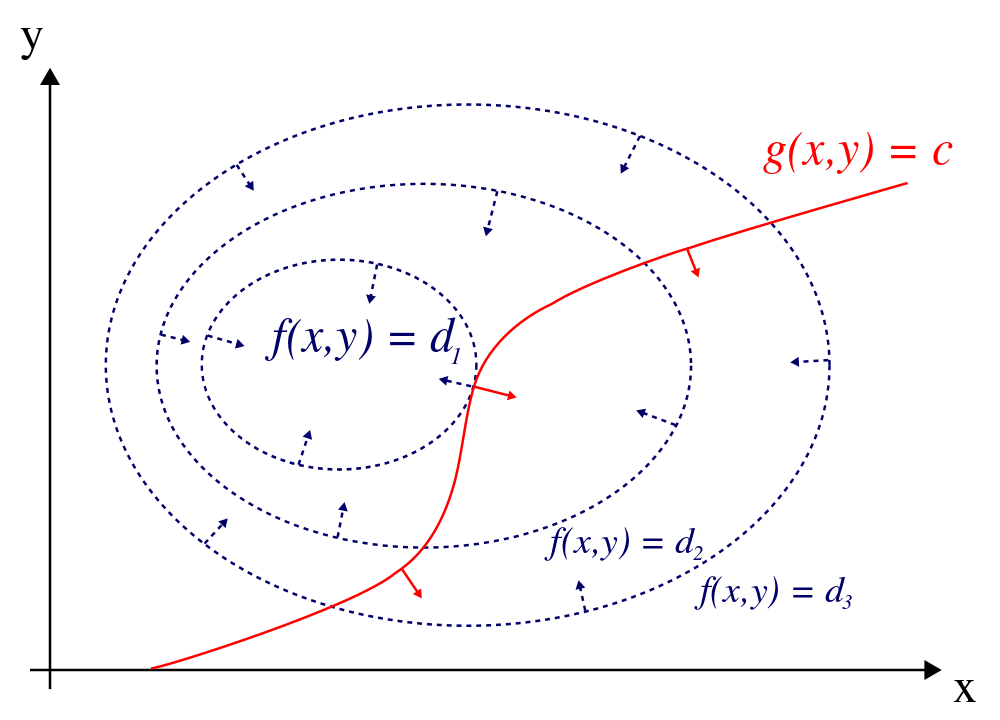
\includegraphics[width=0.6\linewidth]{bilder/08-LagrangeMultipliers2D} 

}

\caption{Schematische Darstellung eines Optimierungsproblems mit Gleichungsnebenbedingungen in 2D.}\label{fig:eqconstraint-opti}
\end{figure}

Wir könnten also versuchen, eine Lösung \((x,y,\lambda)\) für das Gleichungssystem
\begin{equation}
\begin{split}
\nabla f(x, y) + \lambda \nabla g(x, y) &=0 \\
g(x,y) &= c
\end{split}
\label{eq:kkt-sc}
\end{equation}
zu finden.

\leavevmode\hypertarget{lagrange-KKT}{}%
\begin{JHSAYS}
Dieses Gleichungssystem ist ein Spezialfall der \emph{Karush-Kuhn-Tucker} Bedingungen, die ein notwendiges Kriterium für einen optimalen Punkt darstellen. Das involvierte \(\lambda\) wird \emph{Lagrange Multiplikator} genannt.

\end{JHSAYS}

Dass an einem potentiellen Minimum gelten muss, dass \(\nabla f(x^*) = -\lambda \nabla g(x^*)\) haben wir anhand einer Zeichnung im 2D Fall festgestellt.

Für \(x\in \mathbb R^{n}\) und einer Gleichungsnebenbedingung \(g\), ist die Argumentation wie folgt.

\begin{lemma}
\protect\hypertarget{lem:not-para-not-min}{}\label{lem:not-para-not-min}Sei \(x^*\in \mathbb R^{n}\) mit \(g(x^*)=0\) so, dass \(\nabla f\) und \(\nabla g\) \textbf{nicht} parallel sind. Dann gilt für die Richtung
\begin{equation*}
v := -\biggl (I-\frac{1}{\|\nabla g(x^*)\|^2}\nabla g(x^*)g(x^*)^T \biggr )\nabla f(x^*)
\end{equation*}
dass \(\nabla g(x^*)^Tv=0\) und \(\nabla f(x^*)^Tv<0\) ist.
\end{lemma}

Lemma \ref{lem:not-para-not-min} sagt, dass es im skizzierten Fall also eine Richtung gibt, in der (in erster Ableitung) die Funktion \(f\) minimiert werden kann ohne den Zulässigkeitsbereich zu verlassen.

\hypertarget{linear-quadratische-probleme}{%
\section{Linear Quadratische Probleme}\label{linear-quadratische-probleme}}

Ist die Zielfunktion als quadratische Funktion
\begin{equation*}
f(x) = x^T Q x + c^Tx 
\end{equation*}
gegeben mit \(Q\in \mathbb R^{n\times n}\) und \(c\in \mathbb R^{n}\) und sind die Nebenbedingungen linear gegeben als
\begin{equation*}
Ax \geq b
\end{equation*}
mit \(A\in \mathbb R^{m\times n}\), \(b\in \mathbb R^{m}\) und mit \(Ax \geq b\) bedeuten soll, dass \textbf{alle Einträge} des Vektors \(Ax-b\) kleiner oder gleich \(0\) sind, dann sprechen wir von einem (linearen) quadratischen Optimierungsproblem.

Hier müssen Gleichheitsbedingungen nicht explizit angeführt werden, da sie durch Ungleichungsbedingungen ausgedrückt werden können (vgl. \(x=0\) gdw. \(x\geq0\) und \(-x\geq 0\)).

Sind allerdings alle Bedingungen letztlich Gleichheitsbedingungen, liegt also das Problem als
\begin{equation*}
x^T Q x + c^Tx  \to \min_{x\in \mathbb R^{n}} \quad \text{s.t. }Ax=b
\end{equation*}
vor, dann sind die notwendigen Optimalitätsbedingungen durch
\begin{equation*}
\begin{bmatrix}
Q+Q^T & A^T \\
A & 0
\end{bmatrix}
=
\begin{bmatrix}
-c \\ b
\end{bmatrix}.
\end{equation*}

Aus der Betrachtung dieser Optimalitätsbedingungen können wir folgern, dass, wenn \(Q\) symmetrisch ist und positiv definit,
sowie alle Zeilen von \(A\) linear unabhängig sind, dass dann das Optimierungsproblem eine eindeutige Lösung hat, die durch die Optimalitätsbedingungen eindeutig charakterisiert ist.

\hypertarget{sequential-quadratic-programming}{%
\section{Sequential Quadratic Programming}\label{sequential-quadratic-programming}}

Aus der Beobachtung, dass wir LQP Probleme direkt mit \(Q\) symmetrisch positiv definit direkt lösen können und dass wir für kleine Abweichungen \(\xi\) von einem gebenen Punkt \(x\) multivariable Funktionen über quadratische (für unser \(f\)) und lineare Approximationen (für unsere \(g_i\)) gut annähern können:
\begin{equation*}
f(x^*) = f(x+\xi) = f(x) + \nabla f(x)^T \xi + \xi^TH_f(x) \xi + \mathcal o(\| \xi \| ^2 )
\end{equation*}
und
\begin{equation*}
g_i(x^*) = g_i(x+\xi) = g_i(\xi) + \nabla g_i(\xi)^T h + \mathcal o(\| \xi \|), \quad i \in \mathcal I,
\end{equation*}
ergibt sich das folgende iterative Verfahren genannt \emph{Sequential Linear Programming} (SQP):

Beginnend von einem Näherungswert \(x^k\)

\begin{enumerate}
\def\labelenumi{\arabic{enumi}.}
\tightlist
\item
  Berechne \(d^k\) aus der Minimierung von\footnote{Die korrekte quadratische Approximation von \(f\) würde noch den Term \(f(x^k)\) enthalten. Dieser kann aber einfach weggelassen werden bei der Suche der Minimalstelle.}
  \begin{align*}
  \tilde f(x^k+d):= \nabla f(x^k)^T d + d^TH_f(x^k) d \to \min_{d\in \mathbb R^{n}}, \\\quad \text{unter der Nebenbedingung} \\ \tilde g_i(x^k+d):=g(x^k)+\nabla g_i(x^k)d = 0 \quad i \in \mathcal I
    \end{align*}
\item
  ein Update \(x^{k+1}=x^k+d^k\).
\end{enumerate}

Es ist also in jeder Iteration ein linear quadratisches Optimierungsproblem
\begin{equation*}
x^T Q_k x + c_k^Tx  \to \min_{x\in \mathbb R^{n}} \quad \text{s.t. }A_kx=b_k
\end{equation*}
zu lösen, wobei (in der obigen Notation mit \(Q\), \(c\), \(A\) und \(b\)) gilt dass
\begin{equation*}
Q_k=H_f(x^k), \quad c_k=\nabla f(x_k)
\end{equation*}
und
\begin{equation*}
A_k = 
\begin{bmatrix}
\nabla g_i(x_k)^T
\end{bmatrix}_{i \in \mathcal I} \in \mathbb R^{|\mathcal I| \times n},
\quad 
b_k = -
\begin{bmatrix}
g_i(x_k) 
\end{bmatrix}_{i \in \mathcal I}\in \mathbb R^{|\mathcal I|}.
\end{equation*}

\leavevmode\hypertarget{rem-conv-hesse}{}%
\begin{JHSAYS}
Ist die Funktion \(f\) konvex und zweimal stetig differenzierbar (in einer Umgebung von \(x_k\)), dann ist die Hesse-matrix \(H_f(x_k)\) positiv definit und das LQP hat eine eindeutige Lösung \(x_{k+1}\).

\end{JHSAYS}

\hypertarget{aufgaben-5}{%
\section{Aufgaben}\label{aufgaben-5}}

\hypertarget{kkt-fuxfcr-lqp-t}{%
\subsection{KKT für LQP (T)}\label{kkt-fuxfcr-lqp-t}}

Verifizieren Sie, dass die notwendigen Optimalitätsbedingungen für das LQP Problem mit Gleichungsnebenbedingungen (mit \(m=1\)) genau der Optimalitäsbedingung aus Gleichung \eqref{eq:kkt-sc} entspricht. \textbf{Hinweis}: Mit der Definition der \emph{totalen Ableitung} und der Relation zum Gradienten für reellwertige multivariable Funktionen (vgl. die Vorlesung \emph{Mathe für DS2} vom 6. Juli) ist eine Darstellung der Gradienten \(\nabla f(x)\) und \(\nabla g(x)\) direkt herleitbar.

\hypertarget{nicht-parallele-gradienten-t}{%
\subsection{Nicht parallele Gradienten (T)}\label{nicht-parallele-gradienten-t}}

Verifizieren sie die Aussage aus Lemma \ref{lem:not-para-not-min}.

\hypertarget{hauptkomponente-aus-sqp-tp}{%
\subsection{Hauptkomponente aus SQP (T+P)}\label{hauptkomponente-aus-sqp-tp}}

Skizzieren sie das Optimierungsproblems, das die \textbf{letzte} Hauptkomponentenrichtung definiert (also die Richtung mit minimaler Varianz) eines zentrierten Datensatzes definiert (analog dazu, wie in Abschnitt \ref{sec-pca-maximierung} eingeführt). \textbf{Hinweis}: Alles wird vielleicht etwas einfacher, wenn sie die Nebenbedingung \(\|x\|=1\) durch \(\|x\|^2 = 1\) bzw. \$x\^{}Tx = 1 \$ ersetzen. (T)

Skizzieren einen SQP-Schritt zur Lösung dieses Problems. (T)

Implementieren sie die SQP Iteration zur Berechnung der letzten Hauptkomponentenrichtung für die Pinguin Daten. Berechnen Sie die Abweichung zur \emph{exakten} (mit der SVD berechneten) Lösung und geben sie ihn in jedem Schritt beispielsweise den Winkel zwischen dem Iteranten und der exakten Loesung berechnen. \textbf{Hinweis}: Nur die Norm der Differenz könnte irritieren, weil das Vorzeichen der Richtungen nicht festgelegt ist.

\begin{Shaded}
\begin{Highlighting}[]
\ImportTok{import}\NormalTok{ json}
\ImportTok{import}\NormalTok{ numpy }\ImportTok{as}\NormalTok{ np}

\ControlFlowTok{with} \BuiltInTok{open}\NormalTok{(}\StringTok{\textquotesingle{}penguin{-}data.json\textquotesingle{}}\NormalTok{, }\StringTok{\textquotesingle{}r\textquotesingle{}}\NormalTok{) }\ImportTok{as}\NormalTok{ f:}
\NormalTok{    datadict }\OperatorTok{=}\NormalTok{ json.load(f)}

\NormalTok{data }\OperatorTok{=}\NormalTok{ np.array(datadict[}\StringTok{\textquotesingle{}data\textquotesingle{}}\NormalTok{])}

\CommentTok{\# center the data}
\NormalTok{X }\OperatorTok{=}\NormalTok{ data }\OperatorTok{{-}}\NormalTok{ data.mean(axis}\OperatorTok{=}\DecValTok{0}\NormalTok{)}
\NormalTok{XtX }\OperatorTok{=}\NormalTok{ X.T }\OperatorTok{@}\NormalTok{ X  }\CommentTok{\# for later use}

\NormalTok{U, S, Vh }\OperatorTok{=}\NormalTok{ np.linalg.svd(X)}

\NormalTok{pcfour }\OperatorTok{=}\NormalTok{ Vh[}\OperatorTok{{-}}\DecValTok{1}\NormalTok{:, :].T  }\CommentTok{\# die "letzte" Hauptrichtung}
\NormalTok{nrmpcf }\OperatorTok{=}\NormalTok{ np.linalg.norm(pcfour)  }\CommentTok{\# brauchen wir um den Winkel zu berechnen}

\NormalTok{xk }\OperatorTok{=}\NormalTok{ np.zeros((}\DecValTok{4}\NormalTok{, }\DecValTok{1}\NormalTok{))  }\CommentTok{\# Startvektor}
\NormalTok{xk[}\DecValTok{0}\NormalTok{] }\OperatorTok{=} \DecValTok{1}
\NormalTok{arccosalpha }\OperatorTok{=}\NormalTok{ xk.T }\OperatorTok{@}\NormalTok{ pcfour }\OperatorTok{/}\NormalTok{ (np.linalg.norm(xk)}\OperatorTok{*}\NormalTok{nrmpcf)}
\BuiltInTok{print}\NormalTok{(}\SpecialStringTok{f\textquotesingle{}Iteration: }\SpecialCharTok{\{}\DecValTok{0}\SpecialCharTok{\}}\SpecialStringTok{ {-}{-} \textasciigrave{}arccos(sol, xk)\textasciigrave{} }\SpecialCharTok{\{}\NormalTok{arccosalpha}\SpecialCharTok{\}}\SpecialStringTok{\textquotesingle{}}\NormalTok{)}


\KeywordTok{def}\NormalTok{ solve\_sadpoint\_sys\_x(Q}\OperatorTok{=}\VariableTok{None}\NormalTok{, A}\OperatorTok{=}\VariableTok{None}\NormalTok{, fone}\OperatorTok{=}\VariableTok{None}\NormalTok{, ftwo}\OperatorTok{=}\VariableTok{None}\NormalTok{):}
    \CommentTok{\textquotesingle{}\textquotesingle{}\textquotesingle{} Loesung des Sattelpunktprobles}

\CommentTok{    | Q  A.T | . | x |    | f1 |}
\CommentTok{    | A   0  |   | l |  = | f2 |}

\CommentTok{    Notes:}
\CommentTok{    {-}{-}{-}{-}{-}}

\CommentTok{    Es wird nur \textasciigrave{}x\textasciigrave{} zurueckgegeben}

\CommentTok{    \textquotesingle{}\textquotesingle{}\textquotesingle{}}
\NormalTok{    m }\OperatorTok{=}\NormalTok{ A.shape[}\DecValTok{0}\NormalTok{]}
\NormalTok{    lineone }\OperatorTok{=}\NormalTok{ [Q, A.T]}
\NormalTok{    linetwo }\OperatorTok{=}\NormalTok{ [A, np.zeros((m, m))]}
\NormalTok{    sdptmat }\OperatorTok{=}\NormalTok{ np.vstack([np.hstack(lineone),}
\NormalTok{                         np.hstack(linetwo)])}
\NormalTok{    rhs }\OperatorTok{=}\NormalTok{ np.vstack([fone, ftwo])}
\NormalTok{    xl }\OperatorTok{=}\NormalTok{ np.linalg.solve(sdptmat, rhs)}
    \ControlFlowTok{return}\NormalTok{ xl[:}\OperatorTok{{-}}\NormalTok{m]  }\CommentTok{\# return only the \textasciigrave{}x{-}part\textasciigrave{}}


\ControlFlowTok{for}\NormalTok{ kkk }\KeywordTok{in} \BuiltInTok{range}\NormalTok{(}\DecValTok{1}\NormalTok{, }\DecValTok{11}\NormalTok{):}
    \CommentTok{\# ...}
    \CommentTok{\# die SQP Iteration}
    \CommentTok{\# ...}
\NormalTok{    xk }\OperatorTok{=}\NormalTok{ xk }\OperatorTok{+}\NormalTok{ solve\_sadpoint\_sys\_x()}

\NormalTok{    arccosalpha }\OperatorTok{=}\NormalTok{ xk.T }\OperatorTok{@}\NormalTok{ pcfour }\OperatorTok{/}\NormalTok{ (np.linalg.norm(xk)}\OperatorTok{*}\NormalTok{nrmpcf)}
    \BuiltInTok{print}\NormalTok{(}\SpecialStringTok{f\textquotesingle{}Iteration: }\SpecialCharTok{\{}\NormalTok{kkk}\SpecialCharTok{\}}\SpecialStringTok{ {-}{-} \textasciigrave{}arccos(sol, xk)\textasciigrave{} }\SpecialCharTok{\{}\NormalTok{arccosalpha}\SpecialCharTok{\}}\SpecialStringTok{\textquotesingle{}}\NormalTok{)}
\end{Highlighting}
\end{Shaded}

\hypertarget{stochastisches-gradientenverfahren-und-maschinelles-lernen}{%
\chapter{Stochastisches Gradientenverfahren und Maschinelles Lernen}\label{stochastisches-gradientenverfahren-und-maschinelles-lernen}}

\leavevmode\hypertarget{sdg-just-wiki}{}%
\begin{JHSAYS}
Dieses Kapitel ist kopiert (und, teilweise von mir und teilweise automatisch, übersetzt) aus dem Wikipedia Artikel (Stochastistic Gradient, Wikipedia contributors \protect\hyperlink{ref-enwiki:1098148439}{2022}). Dieses Kapitel steht unter der \href{https://en.wikipedia.org/wiki/Wikipedia:Text_of_Creative_Commons_Attribution-ShareAlike_3.0_Unported_License}{\emph{WP:CC BY-SA} Lizenz}.

\end{JHSAYS}

Der stochastische Gradientenabstieg (oft als SGD abgekürzt) ist ein iteratives Verfahren zur Optimierung einer Zielfunktion mit geeigneten Glattheitseigenschaften (z. B. differenzierbar oder subdifferenzierbar). Sie kann als stochastische Näherung der Gradientenabstiegsoptimierung angesehen werden, da sie die tatsächliche Steigung (berechnet aus dem gesamten Datensatz) durch eine Schätzung davon ersetzt (berechnet aus einer zufällig ausgewählten Teilmenge der Daten). Insbesondere bei hochdimensionalen Optimierungsproblemen reduziert dies den sehr hohen Rechenaufwand, wodurch schnellere Iterationen, allerdings im Ausgleich für eine niedrigere Konvergenzrate, erreicht werden.

Während die Grundidee der stochastischen Approximation auf den Robbins-Monro-Algorithmus der 1950er Jahre zurückgeht, hat sich der stochastische Gradientenabstieg zu einer wichtigen Optimierungsmethode im maschinellen Lernen entwickelt.

\hypertarget{hintergrund}{%
\section{Hintergrund}\label{hintergrund}}

Sowohl in der Berechnung statistischer Schätzer als auch im \emph{Maschinellen Lernen} spielt die Minimierung von Zielfunktionalen in Summenform
\begin{equation*}
Q(w) = \frac{1}{N}\sum_{i=1}^N Q_i(w)
\end{equation*}
eine Rolle, wobei der Parameter \(w\in \mathbb R^n\), der
\(Q\) minimiert, gefunden oder geschätzt werden soll.
Jede der Summandenfunktionen \(Q_i\) ist typischerweise assoziiert mit einem \(i\)-ten Datenpunkt (einer Beobachtung) beispielsweise aus einer Menge von Trainingsdaten.

Um obige Funktion zu minimieren, würde ein sogenannter Gradientenabstiegsverfahren den folgenden Minimierungsschritt

\begin{equation*}
w^{k+1} := w^{k} - \eta \nabla Q(w^k) = w^k - \eta \frac{1}{N} \sum_{i=1}^N \nabla Q_i(w^k),
\end{equation*}
iterativ anwenden, wobei \(\eta\) die Schrittweite ist, die besonders in der \emph{ML} community oft auch \emph{learning rate} genannt wird.

Die Berechnung der Abstiegsrichtung erfordert hier also in jedem Schritt die Bestimmung von \(N\) Gradienten \(\nabla Q_i(w^k)\) der Summandenfunktionen. Wenn \(N\) groß ist, also beispielsweise viele Datenpunkte in einer Regression beachtet werden sollen, dann ist die Berechnung entsprechend aufwändig.

Andererseits entspricht die Abstiegsrichtung
\begin{equation*}
\frac{1}{N} \sum_{i=1}^N \nabla Q_i(w^k)
\end{equation*}
dem Mittelwert der Gradienten aller \(Q_i\)s am Punkt \(w_k\), der durch ein kleineres Sample

\begin{equation*}
\frac{1}{N} \sum_{i=1}^N \nabla Q_i(w^k) \approx \frac{1}{|\mathcal J|} \sum_{j\in \mathcal J} \nabla Q_j(w^k),
\end{equation*}

wobei \(\mathcal J \subset \{1, \dotsc, N\}\) eine Indexmenge ist, die den \emph{batch} der zur Approximation gewählten \(Q_i\)s beschreibt.

\hypertarget{iterative_method}{%
\section{Stochastisches Abstiegsverfahren}\label{iterative_method}}

Beim stochastischen (oder ``Online'') Gradientenabstieg wird der wahre Gradient von \(Q(w^k)\) durch einen Gradienten bei einer einzelnen Probe angenähert:
\begin{equation*}
w^{k+1} = w^k-\eta \nabla Q_j(w^k),
\end{equation*}
mit \(j\in \{1,\dotsc, N\}\) zufällig gewählt (ohne zurücklegen).

Während der Algorithmus den Trainingssatz durchläuft, führt er die obige Aktualisierung für jede Trainingsprobe durch. Es können mehrere Durchgänge über den Trainingssatz gemacht werden, bis der Algorithmus konvergiert. Wenn dies getan wird, können die Daten für jeden Durchlauf gemischt werden, um Zyklen zu vermeiden. Typische Implementierungen können eine adaptive Lernrate verwenden, damit der Algorithmus konvergiert.

Die wesentlichen Schritte als Algorithmus sehen wie folgt aus:

\begin{Shaded}
\begin{Highlighting}[]
\CommentTok{\#\#\#\#\#\#\#\#\#\#\#\#\#\#\#\#\#\#\#\#\#\#\#\#\#\#\#\#\#\#\#\#\#\#\#\#\#\#\#\#\#\#\#\#\#\#\#\#\#\#\#}
\CommentTok{\# The basic steps of a stochastic gradient method \#}
\CommentTok{\#\#\#\#\#\#\#\#\#\#\#\#\#\#\#\#\#\#\#\#\#\#\#\#\#\#\#\#\#\#\#\#\#\#\#\#\#\#\#\#\#\#\#\#\#\#\#\#\#\#\#}

\NormalTok{w }\OperatorTok{=}\NormalTok{ ...  }\CommentTok{\# initialize the weight vector}
\NormalTok{eta }\OperatorTok{=}\NormalTok{ ... }\CommentTok{\# choose the learning rate}
\NormalTok{I }\OperatorTok{=}\NormalTok{ [}\DecValTok{1}\NormalTok{, }\DecValTok{2}\NormalTok{, ..., N]  }\CommentTok{\# the full index set}

\ControlFlowTok{for}\NormalTok{ k }\KeywordTok{in} \BuiltInTok{range}\NormalTok{(maxiter):}
\NormalTok{    J }\OperatorTok{=}\NormalTok{ shuffle(I)  }\CommentTok{\# shuffle the indices}
    \ControlFlowTok{for}\NormalTok{ j }\KeywordTok{in}\NormalTok{ J:}
        \CommentTok{\# compute the gradient of Qj at current w}
\NormalTok{        gradjk }\OperatorTok{=}\NormalTok{ nabla(Q(j, w))  }
        \CommentTok{\# update the w vector}
\NormalTok{        w }\OperatorTok{=}\NormalTok{ w }\OperatorTok{{-}}\NormalTok{ eta}\OperatorTok{*}\NormalTok{gradjk}
    \ControlFlowTok{if}\NormalTok{ convergence\_criterion:}
       \ControlFlowTok{break}

\CommentTok{\#\#\#\#\#\#\#\#\#\#\#\#\#\#\#\#\#\#\#\#\#\#\#\#\#\#\#\#\#\#\#\#\#\#\#\#\#\#\#\#\#\#\#\#\#\#\#\#\#\#\#}
\end{Highlighting}
\end{Shaded}

Die Konvergenz des \emph{stochastischen Gradientenabstiegsverfahren} als Kombination von \emph{stochastischer Approximation} und \emph{numerischer Optimierung} ist gut verstanden. Allgemein und unter bestimmten Voraussetzung lässt sich sagen, dass das stochastische Verfahren ähnlich konvergiert wie das \emph{exakte Verfahren} mit der Einschränkung, dass die Konvergenz \emph{fast sicher} stattfindet.

In der Praxis hat sich der Kompromiss etabliert, der anstelle des Gradienten eines einzelnen Punktes \(\nabla Q_j(w_k)\), den Abstieg aus dem Mittelwert über mehrere Samples berechnet, also (wie oben beschrieben)
\begin{equation*}
\frac{1}{N} \sum_{i=1}^N \nabla Q_i(w^k) \approx \frac{1}{|\mathcal J|} \sum_{j\in \mathcal J} \nabla Q_j(w^k).
\end{equation*}
Im Algorithmus wird dann anstelle der zufälligen Indices \(j \in \{1, \dotsc, N\}\), über zufällig zusammengestellte Indexmengen \(\mathcal J \subset \{1, \dotsc, N\}\) iteriert.

Da die einzelnen Gradienten \(\nabla Q_j(w^K)\) unabhängig voneinander berechnet werden können, kann so ein \emph{batch} Verfahren effizient auf Computern mit mehreren Prozessoren realisiert werden. Die Konvergenztheorie ist nicht wesentlich verschieden vom eigentlichen \emph{stochastischen Gradientenabstiegsverfahren}, allerdings erscheint die beobachte Konvergenz weniger erratisch, da der Mittelwert statistische Ausreißer ausmitteln kann.

\hypertarget{aufgabe}{%
\section{Aufgabe}\label{aufgabe}}

Schreiben Sie ein Programm, das mit Hilfe eines neuronalen Netzes (NN) mit einer \emph{hidden layer}
\begin{equation*}
\eta_i = NN(x_i):=\tanh \bigl (A_2 \tanh (A_1 x_i + b_1) + b_2\bigr )
\end{equation*}

für einen Datenpunkt \(x_i \in \mathbb R^{n_0}\), Gewichten \(A_1 \in \mathbb R^{n_1 \times n_0}\), \(b_1 \in \mathbb R^{n_1}\), \(A_2 \in \mathbb R^{1, n_1}\), \(b_2 \in \mathbb R^{1}\) und dem Ergebnisvektor \(\eta_i\in \mathbb R^{1}\), anhand der gemessenen Daten \(x_i\) die bekannte Pinguin Population \href{bilder/penguin-data.json}{\texttt{penguin-data.json}} in zwei Gruppen aufteilt, so dass in der ersten Gruppe eine Spezies enthalten ist und in der anderen die beiden anderen Spezies.

Dazu kann eine Funktion \(\ell \colon X \mapsto \{-1, 1\}\) definiert werden, die die bekannten Pinguine \(x_i\) aus dem Datensatz \(X\) ihrer Gruppe zuordnet. Dann können die Koeffizienten des \(NN\) über das Optimierungsproblem
\begin{equation*}
\frac{1}{|X|}\sum_{x_i \in X} \|\ell(x_i)-NN(x_i)\|^2 \to \min_{A_1, b_1, A_2, b_2}
\end{equation*}
mittels des \emph{stochastischen (batch) Gradientenabstiegs} bestimmt werden.

\textbf{Hinweis}: Für eine Funktion \(f \colon w \mapsto f(w) \in \mathbb R\), können sie den Gradienten \(\nabla_w f(w^*)\) an der Stelle \(w^*\) numerisch mit der Funktion \texttt{scipy.optimize.approx\_fprime} bestimmen lassen.

Führen Sie die Optimierung auf einem Teil (z.B. 90\%) der Pinguin Daten durch und testen sie wie gut ihr Netz funktioniert auf den verbleibenden Datenpunkten.

Der Beginn könnte also wie folgt aussehen (wobei die Größe der \emph{hidden layer} zu \(n_1=2\) gesetzt ist).

\begin{Shaded}
\begin{Highlighting}[]
\ImportTok{import}\NormalTok{ json}
\ImportTok{import}\NormalTok{ numpy }\ImportTok{as}\NormalTok{ np}
\ImportTok{from}\NormalTok{ scipy.optimize }\ImportTok{import}\NormalTok{ approx\_fprime}

\ControlFlowTok{with} \BuiltInTok{open}\NormalTok{(}\StringTok{\textquotesingle{}penguin{-}data.json\textquotesingle{}}\NormalTok{, }\StringTok{\textquotesingle{}r\textquotesingle{}}\NormalTok{) }\ImportTok{as}\NormalTok{ f:}
\NormalTok{    datadict }\OperatorTok{=}\NormalTok{ json.load(f)}

\NormalTok{data }\OperatorTok{=}\NormalTok{ np.array(datadict[}\StringTok{\textquotesingle{}data\textquotesingle{}}\NormalTok{])}
\CommentTok{\# centering the data}
\NormalTok{data }\OperatorTok{=}\NormalTok{ data }\OperatorTok{{-}}\NormalTok{ data.mean(axis}\OperatorTok{=}\DecValTok{0}\NormalTok{)}
\NormalTok{lbls }\OperatorTok{=}\NormalTok{ np.array(datadict[}\StringTok{\textquotesingle{}target\textquotesingle{}}\NormalTok{])}

\CommentTok{\# a dictionary that maps the labels(=targets) of the data into labels \{1, {-}1\}}
\CommentTok{\# that will use for distinction of two groups}
\NormalTok{mplbldict }\OperatorTok{=}\NormalTok{ \{}\DecValTok{0}\NormalTok{: np.array([}\OperatorTok{{-}}\DecValTok{1}\NormalTok{]),}
             \DecValTok{1}\NormalTok{: np.array([}\OperatorTok{{-}}\DecValTok{1}\NormalTok{]),}
             \DecValTok{2}\NormalTok{: np.array([}\DecValTok{1}\NormalTok{])\}}

\CommentTok{\# sizes of the layers}
\NormalTok{sxz, sxo, sxt }\OperatorTok{=}\NormalTok{ data.shape[}\DecValTok{1}\NormalTok{], }\DecValTok{2}\NormalTok{, mplbldict[}\DecValTok{0}\NormalTok{].size}
\CommentTok{\# define also the sizes of the weightmatrices}

\CommentTok{\# parameters for the training {-}{-} these worked fine for me}
\NormalTok{batchsize }\OperatorTok{=} \DecValTok{30}  \CommentTok{\# how many samples for the stochastic gradients}
\NormalTok{lr }\OperatorTok{=} \FloatTok{0.25}  \CommentTok{\# learning rate}
\NormalTok{iterations }\OperatorTok{=} \DecValTok{200}  \CommentTok{\# how many gradient steps}

\CommentTok{\# the data}
\NormalTok{traindataratio }\OperatorTok{=} \FloatTok{.9}  \CommentTok{\# the ratio of training data vs. test data}
\NormalTok{ndata }\OperatorTok{=}\NormalTok{ data.shape[}\DecValTok{0}\NormalTok{]}
\NormalTok{trnds }\OperatorTok{=}\NormalTok{ np.}\BuiltInTok{int}\NormalTok{(ndata}\OperatorTok{*}\NormalTok{traindataratio)}
\NormalTok{allidx }\OperatorTok{=}\NormalTok{ np.arange(ndata)}
\NormalTok{trnidx }\OperatorTok{=}\NormalTok{ np.random.choice(allidx, trnds, replace}\OperatorTok{=}\VariableTok{False}\NormalTok{)}
\NormalTok{tstidx }\OperatorTok{=}\NormalTok{ np.setdiff1d(allidx, trnidx)}
\end{Highlighting}
\end{Shaded}

Und die Funktion, die das neuronale Netz realisiert, so:

\begin{Shaded}
\begin{Highlighting}[]
\KeywordTok{def}\NormalTok{ fwdnn(xzero, Aone}\OperatorTok{=}\VariableTok{None}\NormalTok{, bone}\OperatorTok{=}\VariableTok{None}\NormalTok{, Atwo}\OperatorTok{=}\VariableTok{None}\NormalTok{, btwo}\OperatorTok{=}\VariableTok{None}\NormalTok{):}
    \CommentTok{\textquotesingle{}\textquotesingle{}\textquotesingle{} a neural networks of two layers}

\CommentTok{    \textquotesingle{}\textquotesingle{}\textquotesingle{}}
\NormalTok{    xone }\OperatorTok{=}\NormalTok{ np.tanh(Aone }\OperatorTok{@}\NormalTok{ xzero }\OperatorTok{+}\NormalTok{ bone)}
\NormalTok{    xtwo }\OperatorTok{=}\NormalTok{ np.tanh(Atwo }\OperatorTok{@}\NormalTok{ xone }\OperatorTok{+}\NormalTok{ btwo)}
    \ControlFlowTok{return}\NormalTok{ xtwo}
\end{Highlighting}
\end{Shaded}

Für die Umsetzung ist es hilfreich, alle Koeffizienten in einen Vektor \(w\) vorzuhalten. Damit kann dann optimiert werden und bei Bedarf die Matrizen wieder hergestellt werden:

\begin{Shaded}
\begin{Highlighting}[]
\KeywordTok{def}\NormalTok{ wvec\_to\_wmats(wvec):}
    \CommentTok{\textquotesingle{}\textquotesingle{}\textquotesingle{} helper to turn the vector of weights into the system matrices}

\CommentTok{    \textquotesingle{}\textquotesingle{}\textquotesingle{}}
\NormalTok{    Aone }\OperatorTok{=}\NormalTok{ wvec[:sxz}\OperatorTok{*}\NormalTok{sxo].reshape((sxo, sxz))}
\NormalTok{    cidx }\OperatorTok{=}\NormalTok{ sxz}\OperatorTok{*}\NormalTok{sxo}
\NormalTok{    bone }\OperatorTok{=}\NormalTok{ wvec[cidx:cidx}\OperatorTok{+}\NormalTok{sxo]}
\NormalTok{    cidx }\OperatorTok{=}\NormalTok{ cidx }\OperatorTok{+}\NormalTok{ sxo}
\NormalTok{    Atwo }\OperatorTok{=}\NormalTok{ wvec[cidx:cidx}\OperatorTok{+}\NormalTok{sxo}\OperatorTok{*}\NormalTok{sxt].reshape((sxt, sxo))}
\NormalTok{    cidx }\OperatorTok{=}\NormalTok{ cidx }\OperatorTok{+}\NormalTok{ sxo}\OperatorTok{*}\NormalTok{sxt}
\NormalTok{    btwo }\OperatorTok{=}\NormalTok{ wvec[cidx:]}
    \ControlFlowTok{if}\NormalTok{ Aone.size }\OperatorTok{+}\NormalTok{ bone.size }\OperatorTok{+}\NormalTok{ Atwo.size }\OperatorTok{+}\NormalTok{ btwo.size }\OperatorTok{==}\NormalTok{ wvec.size:}
        \ControlFlowTok{return}\NormalTok{ Aone, bone, Atwo, btwo}
    \ControlFlowTok{else}\NormalTok{:}
        \ControlFlowTok{raise} \PreprocessorTok{UserWarning}\NormalTok{(}\StringTok{\textquotesingle{}mismatch weightsvector/matrices\textquotesingle{}}\NormalTok{)}
\end{Highlighting}
\end{Shaded}

Damit fehlen zum Programm insbesondere noch

\begin{itemize}
\tightlist
\item
  die Zielfunktion der Optimierung in einem Datenpunkt \(x_i\)
\item
  eine Funktion, die den stochastischen Gradienten über einem kleinen \emph{batch} von Daten ausrechnet
\item
  eine Iteration, die das Gradientenabstiegsverfahren zusammen mit der \emph{learning rate} durchführt
\item
  ein Loop, der testet, wie das optimierte \(NN\), die verbliebenen Daten klassifiziert
\end{itemize}

\textbf{Hinweis}: Auch hier ist wieder sehr viel Zufall involviert. Im Zweifel lieber zweimal testen.

\textbf{Hinweis}: Der letzte Testloop könnte so aussehen:

\begin{Shaded}
\begin{Highlighting}[]
\BuiltInTok{print}\NormalTok{(}\StringTok{\textquotesingle{}***** testing the classification *****\textquotesingle{}}\NormalTok{)}
\NormalTok{faillst }\OperatorTok{=}\NormalTok{ []  }\CommentTok{\# list to collect the failures for later examination}
\ControlFlowTok{for}\NormalTok{ cti }\KeywordTok{in}\NormalTok{ tstidx:  }\CommentTok{\# iteration over the test data points}
\NormalTok{    itrgt }\OperatorTok{=}\NormalTok{ data[cti, :]}
\NormalTok{    ilbl }\OperatorTok{=}\NormalTok{ mplbldict[lbls[cti]]}
    \CommentTok{\# the prediction of the neural network {-}{-} Aonex, ... are the optimized weights}
\NormalTok{    nnlbl }\OperatorTok{=}\NormalTok{ fwdnn(itrgt, Aone}\OperatorTok{=}\NormalTok{Aonex, bone}\OperatorTok{=}\NormalTok{bonex, Atwo}\OperatorTok{=}\NormalTok{Atwox, btwo}\OperatorTok{=}\NormalTok{btwox)}
\NormalTok{    sccs }\OperatorTok{=}\NormalTok{ np.sign(ilbl) }\OperatorTok{==}\NormalTok{ np.sign(nnlbl)}
    \BuiltInTok{print}\NormalTok{(}\SpecialStringTok{f\textquotesingle{}label: }\SpecialCharTok{\{}\NormalTok{ilbl}\SpecialCharTok{.}\NormalTok{item()}\SpecialCharTok{\}}\SpecialStringTok{ {-}{-} nn: }\SpecialCharTok{\{}\NormalTok{nnlbl}\SpecialCharTok{.}\NormalTok{item()}\SpecialCharTok{:.4f\}}\SpecialStringTok{ {-}{-} success: }\SpecialCharTok{\{}\NormalTok{sccs}\SpecialCharTok{\}}\SpecialStringTok{\textquotesingle{}}\NormalTok{)}
    \ControlFlowTok{if} \KeywordTok{not}\NormalTok{ sccs:}
\NormalTok{        faillst.append((cti, ilbl.item(), nnlbl.item(),}
\NormalTok{                        datadict[}\StringTok{\textquotesingle{}target\_names\textquotesingle{}}\NormalTok{][lbls[cti]]))}
    \ControlFlowTok{else}\NormalTok{:}
        \ControlFlowTok{pass}

\BuiltInTok{print}\NormalTok{(}\StringTok{\textquotesingle{}}\CharTok{\textbackslash{}n}\StringTok{***** Results *****\textquotesingle{}}\NormalTok{)}
\BuiltInTok{print}\NormalTok{(}\SpecialStringTok{f\textquotesingle{}}\SpecialCharTok{\{}\DecValTok{100}\OperatorTok{{-}}\BuiltInTok{len}\NormalTok{(faillst)}\OperatorTok{/}\NormalTok{tstidx}\SpecialCharTok{.}\NormalTok{size}\OperatorTok{*}\DecValTok{100}\SpecialCharTok{:.0f\}}\SpecialStringTok{\% was classified correctly\textquotesingle{}}\NormalTok{)}
\BuiltInTok{print}\NormalTok{(}\StringTok{\textquotesingle{}***** Misses *****\textquotesingle{}}\NormalTok{)}
\ControlFlowTok{if} \BuiltInTok{len}\NormalTok{(faillst) }\OperatorTok{==} \DecValTok{0}\NormalTok{:}
    \BuiltInTok{print}\NormalTok{(}\StringTok{\textquotesingle{}None\textquotesingle{}}\NormalTok{)}
\ControlFlowTok{else}\NormalTok{:}
    \ControlFlowTok{for}\NormalTok{ cfl }\KeywordTok{in}\NormalTok{ faillst:}
\NormalTok{        cid, lbl, nnlbl, name }\OperatorTok{=}\NormalTok{ cfl}
        \BuiltInTok{print}\NormalTok{(}\SpecialStringTok{f\textquotesingle{}ID: }\SpecialCharTok{\{}\NormalTok{cid}\SpecialCharTok{\}}\SpecialStringTok{ (}\SpecialCharTok{\{}\NormalTok{name}\SpecialCharTok{\}}\SpecialStringTok{ pinguin) was missclassified \textquotesingle{}} \OperatorTok{+}
              \SpecialStringTok{f\textquotesingle{}with score }\SpecialCharTok{\{}\NormalTok{nnlbl}\SpecialCharTok{:.4f\}}\SpecialStringTok{ vs. }\SpecialCharTok{\{}\NormalTok{lbl}\SpecialCharTok{\}}\SpecialStringTok{\textquotesingle{}}\NormalTok{)}
\end{Highlighting}
\end{Shaded}

\hypertarget{referenzen}{%
\chapter*{Referenzen}\label{referenzen}}
\addcontentsline{toc}{chapter}{Referenzen}

\hypertarget{refs}{}
\begin{cslreferences}
\leavevmode\hypertarget{ref-BolM04}{}%
Bollhöfer, M., Mehrmann, V.: Numerische Mathematik. Eine projektorientierte Einführung für Ingenieure, Mathematiker und Naturwissenschaftler. Vieweg (2004)

\leavevmode\hypertarget{ref-NocW06}{}%
Nocedal, J., Wright, S.J.: Numerical optimization. Springer (2006)

\leavevmode\hypertarget{ref-enwiki:1098148439}{}%
Wikipedia contributors: Stochastic gradient descent --- Wikipedia, the free encyclopedia, \url{https://en.wikipedia.org/w/index.php?title=Stochastic_gradient_descent\&oldid=1098148439}, (2022)
\end{cslreferences}

\end{document}
